\documentclass[letterpaper, 10pt, openright]{memoir}

%0ther
\renewcommand{\and}{\\\vskip 1em}
\def\headline#1{\hbox to \hsize{\hrulefill\quad\lower.3em\hbox{#1}\quad\hrulefill}}
\newcommand{\doendnotes}{%
	\markright{Notes}
	\theendnotes
	\setcounter{endnote}{0}
}
\newcommand{\doubleline}{%
	\hrule height 3\normalrulethickness
	\vskip 0.25em
	\hrule height \normalrulethickness
}

%Table of Contents
\makeatletter
\def\cftsectionpresnum #1\@cftasnum{}
\makeatother
\setlength\cftchapternumwidth{3em}
\cftpagenumbersoff{chapter}
\renewcommand{\contentsname}{\huge{Table} \Large{of} \huge{Contents}}

%Chapter style
\makechapterstyle{custom} {%
	\renewcommand{\thechapter}{\Roman{chapter}}
	\renewcommand{\chapterheadstart}{}
	\renewcommand{\printchaptername}{}
	\renewcommand{\chapternamenum}{}
	\renewcommand{\printchapternum}{\headline{\huge Chapter \thechapter}}
	\renewcommand{\afterchapternum}{}
	\renewcommand{\printchaptertitle}[1]{%
		\raggedright\huge\scshape\MakeLowercase{##1}}
	\renewcommand{\afterchaptertitle}{%
		\vskip\onelineskip \hrule\vskip\onelineskip}
}
\chapterstyle{custom}

%Section
\renewcommand{\thesection}{\Roman{section}}
\setsecheadstyle{\raggedright\scshape\large}
\setbeforesecskip{-\onelineskip}
\setaftersecskip{\onelineskip}
\setsecnumformat{}
\renewcommand{\sectionmark}[1]{\markboth{Chapter \thechapter.}{Part \thesection.}}

%subsection
\setsubsecheadstyle{\sethangfrom{\noindent ##1}\raggedright\itshape}
\setbeforesubsecskip{-\onelineskip}
\setaftersubsecskip{\onelineskip}

%EndNotes
\makepagenote
\renewcommand{\idtextinnotes}[1]{\footnotesize#1)\space}
\renewcommand{\prenoteinnotes}{\par\noindent\hangindent 2em}
\renewcommand{\prenotetext}{\begingroup\footnotesize}
\renewcommand{\postnotetext}{\endgroup}
\renewcommand{\notedivision}{%
	\headline{\huge\notesname}\vskip\onelineskip
	\markboth{Chapter \thechapter.}{\notesname}
	\thispagestyle{simple}
}
\renewcommand{\pagenotesubhead}[3]{}

\begin{document}
\frontmatter
\pretitle{\begin{center}\bfseries}
\title{%
	\small{THE}\\\vskip 1em
	\Huge{HISTORY}\\\vskip 1em
	\small{OF THE}\\\vskip 1em
	\Large{DECLINE AND FALL}\\\vskip 1em
	\small{OF THE}\\\vskip 1em
	\Huge{ROMAN EMPIRE}
}
\posttitle{\end{center}\vskip 1em}
\preauthor{\begin{center}\large\bfseries}
\author{%
	Edward Gibbon, \textit{Esq.}
	\and  With notes by the Rev. H. H. Milman
	\and Vol. 1}
\postauthor{\end{center}}
\predate{\begin{center}}
\date{\bfseries\normalsize 1782 (Written), 1845 (Revised)}
\postdate{%
	\end{center}
	\vskip 1em
	\doubleline
}

\maketitle


\tableofcontents*
\begin{flushleft}
\fontsize{35}{35}\sffamily
\textbf{Man, His Origin and Destiny}
\Large{by Joseph Fielding Smith}
\end{flushleft}

\section{FOREWORD}
\thispagestyle{empty}

Conflicting attitudes expressed concerning science and religion have confused many people.
Especially has this been true in the class room where hypotheses have been set forth
erroneously as facts and where deductions made from those theories have been regarded as
established truth.

Many of the followers of Darwin, for instance, carried his views to the extreme of
materialistic atheism, declaring not only that creation occurred without the aid of any
Intelligent Creator, but that as a matter of fact, no such Being even exists.
Both science and religion have suffered as a result. The greatest damage, however, has been
among students who have lost their faith in God through accepting these man-made theories
as facts.

But time changes things. Whereas for years atheistic deductions were made from scientific
research, now true scientists, armed with what they term "the new knowledge," are revising
their "hasty first conclusions" as Sir James Jeans expressed it, and have discovered "evidence
of a designing or controlling power that has something in common with our individual
minds."

The present day attitude of top scientists was expressed recently by Dr. Joseph W. Barker,
president and chairman of the Research Corporation of America, and formerly dean of the
engineering school at Columbia University, in an address at Ripon University. He explained
there that scientists of the nineteenth century were misled by certain of their observations,
and as a result came to conclusions which were definitely atheistic.

"But now," said Dr. Barker, "even the most pragmatic materialist, in the face of present day
scientific knowledge, is led to the inevitable conclusion that the heavens declare the glory of
God and the firmament showeth his handiwork."

Dr. Barker's concluding remarks to the students were: "As the children of Israel foreswore
the worship of the golden calf and returned to the faith of Jehovah, so have we foresworn the
crass mechanistic materialism and returned to that faith in God of which the Psalmist of old
sang. The Earth is the Lord's and all that therein is."

Knowing the great need to provide Latter-day Saint students of science with material which
would help them to preserve their faith and coordinate in their minds the pure truth of both
science and revelation, some of us have hoped for a book which could make the facts readily
available to them.

Many have recognized in President Joseph Fielding Smith of the Council of the Twelve the
profound student of scripture which he is, but not so many were acquainted with the fact that
he also is a deep student of science, widely read in various phases of the subject.

Recognizing his possession of this superb knowledge of both science and religion, some of
us urged him to write a book on the creation of the world and the origin of man, setting forth
both the up-to-date views of science, and the facts provided through revelation.

The present volume is the result. It is a most remarkable presentation of material from both
sources under discussion. It will fill a great need in the Church, and will be particularly
invaluable to students who have become confused by the misapplication of information
derived from scientific experimentation.

It will be an outstanding addition to a list of this author's books which already have stabilized
the faith of countless thousands the world around.

\vspace{\onelineskip}
-MARK E. PETERSEN.

\newpage
\section{AN INTRODUCTION}

\begin{flushleft}
BY DR. MELVIN A. COOK
\end{flushleft}

Theory plays an important role in all arts and sciences (1) by providing a means for the
unification and classification of available knowledge, and (2) by suggesting and prescribing
the design of experimental studies that will broaden the scope of knowledge. Failure to
accomplish either of these objectives necessitates modifications in the theory or substitution
of an alternate one. For this reason the basic concepts are continually undergoing change in a
healthy and forward-moving science. We are living in a world of great endeavor and
achievement in which the scientific or objective application of theory, whether true or simply
the best that can be devised to represent as faithfully as possible all known facts, has an
important place. Unfortunately, owing to the strong desire of scientists to display their
brilliance and ingenuity, there is a tendency for theory to become the objective instead of a
means to the end. Theory then not only loses its real value, but actually becomes a stumbling
block to progress. Its inventor and disciples become so engrossed in the theory that they lose
sight of its fundamental purpose, the quest for truth. This condition was shockingly
illustrated in my presence at a meeting of scientists when one of great renown met a factual
objection with the statement, "I am more concerned with the elegance of the theory than the
truth of it."

One need not look far into science to discover it consists too generally of a maze of facts and
theory so closely interwoven that even the most learned and honorable scientist (to say
nothing of the intellectually dishonest one or the novice) may have difficulty in
distinguishing readily between truth and theory. While this weakness of science is serious
enough in fields which are not closely related to the primary purposes of mortality, in the
fields more closely related, the difficulties of discerning fact and theory may well prove
disastrous. This is particularly true as regards the development of spirituality in those who
place science foremost.

The principles of the Gospel of Jesus Christ provide faithful members of the Church with
wonderful and inspiring principles of truth directly applicable in distinguishing between
fundamental truth and error in all fields of arts and science. This application requires a clear
recognition of the pre-eminence of the gospel and its "eternal scientists" of which the author
of this book stands high among the great ones in mortality. The paramount key to this
important application of "eternal science" is that every principle of the baser sciences must
square with the revealed truths.

Few fields of science come into such direct conflict with the revealed scriptures as the
palaeo-sciences—historical geology, palaeoethnology, paleontology, and palaeogeography.
The factual or experimental components of these sciences have contributed much to our
knowledge and culture and their scientists are indispensable in practical applications dealing
with the structural and dynamic features of the earth's crust, the discovery of valuable
minerals and the evaluation of natural resources, and description and classification of plants
and animals. With the author of this book, I believe that much of the theoretical structure of
these sciences is incorrect because it is not only in disagreement with the scriptures but is in
direct opposition to them. Moreover, I believe that when these sciences are denuded of their
theoretical superstructure, they are not found to conflict with the revealed truths of thescriptures.
For those who have the patience to await the great event, when the final chapters
of theory in these and other sciences are written, I am confident that they also will square
with the pre-eminent science of our Savior. The great challenge thus confronts the scientist
with faith in divine revelation to attempt each in his own field to write his theories to include
not only the facts of direct experimental observation but also those generally more significant
ones revealed by the Omnipotent Scientist, the Creator of the world and Savior of mankind.

As one frequently confronted with questions from perplexed students of the sciences, I am
deeply grateful for this documental and scientifically accurate volume to which one may turn
for answers to technical questions as well as for inspiration to continue steadfast in the
gospel. This study reveals its author to be one well versed in the scientific method and a
strong supporter of true science and those scientists who apply theory and observation
objectively in the search for truth and toward creative contributions to civilization. If he
seems impatient toward those whose objective is elegance in the manipulation of theory
rather than the discovery of truth, it is because of his deep love for mankind and a passion to
see him on the way to eternal life.

\vspace{\onelineskip}
MELVIN A. COOK

\vspace{\onelineskip}
Professor of Metallurgy

\vspace{\onelineskip}
University of Utah

\newpage
\section{PREFACE}
The following pages are the result of many months of reflection and conviction that
something should be written to strengthen the faith of some weak members of the Church,
and our students in the public schools and colleges, who are constantly exposed to the
theories of organic evolution and the higher criticism, so-called.

These hypotheses are not confined to the schools, for they find their way into the press and
current magazines expressed with a finality as though they had been definitely proved. They
are but guesses. They can never be more than guesses, for they lie beyond the possibility of
proof. Moreover, being in conflict with the revelations of the Lord to his servants the
prophets, and the teachings of our Redeemer, they are ever destructive of faith.

It has been my wish for several years that something might be done to counteract these false
teachings, so destructive of faith in God. I have mentioned this many times to my associates
and it is with their constant urging that I have undertaken this work.

To Elders Mark E. Petersen, Marion G. Romney of the Council of the Twelve; Elders Milton
R. Hunter and Bruce R. McConkie of the First Council of Seventy, I am deeply indebted for
the encouragement and help which they have given. Equally am I indebted to Dr. Melvin A.
Cook and Elder A. Wm. Lund, assistant Church Historian, for their assistance and their
valuable suggestions. Nor must I forget the aid of my secretary, Mrs. Rubie McKinlay
Egbert, and my wife, Jessie Evans Smith, for the typing and reading of the proof, and my
son, Joseph Fielding Smith Jr., who set the type and offered many helpful suggestions.

\vspace{\onelineskip}
—JOSEPH FIELDING SMITH.

\newpage
\section{ACKNOWLEDGMENTS}
Sincere appreciation and thanks are given to the following publishers for the privilege
granted to use quotations from the copyright works here listed which have been of great
assistance in the publication of this work.

The Victoria Institute or Philosophical Society of Great Britain, for numerous quotations
from several volumes of the \textit{Journal of Transactions}, including the entire lecture of Dr.
Albert Fleischmann, professor of Zoology and Comparative Anatomy in the University of
Erlangen, Germany, Volume 65, for the year 1933.

Augsburg Publishing House, Minneapolis: \textit{After Its Kind} and \textit{The Deluge Story in Stone}, by
Byron C. Nelson.

Pacific Press Publishing Association, Mountain View, California: \textit{The New Geology}, by
Professor George McCready Price.

The Devin-Adair Company, New York: \textit{God—Or Gorilla}, by Alfred Watterson McCann.

Funk \& Wagnalls Company, New York and London: \textit{The New Archaeological Discoveries},
Dr. Camden M. Cobern.

William Heinemann Ltd., London: \textit{The Accuracy of the Bible}, Dr. A. S. Yahuda.

Fleming H. Revell Company, London and Edinburgh: \textit{New Bible Evidences}, Sir Charles
Marston.

The following works, in addition to those mentioned above, will be of great benefit to any
who are confused by the hypothesis of organic evolution:

\textit{The Mammoth and the Flood; The Glacial Nightmare and the Flood}, (two volumes); \textit{Ice or
Water}, (two volumes), by Sir Henry Howorth.

\textit{The Phantom of Organic Evolution; The Geological Hoax}, by Professor George McCready
Price.

\textit{The Origin of Mankind; Evolution or Creation}, Sir Ambrose Fleming.

\newpage
\section{INTRODUCTION}

FOR a long time I have wished that someone more capable than I would write a defense of
the fundamental principles of the Gospel for the benefit of our youth who are confronted in
their studies in high schools and universities with the modern theories of so-called science
and philosophy which are in conflict with the revealed doctrines of the Church. I realize that
many books and articles have been published in defense of the faith, but not one that deals
with these pernicious doctrines which have become so universally accepted even in what we
are pleased to call our Christian nation. There cannot be any conflict between truth revealed
from heaven and truth revealed through the research of man; for truth is a unit and never is
found in conflict with itself. Unfortunately we live in an age when many theories which have
not been proved are accepted as truth. These theories have been changed from time to time
and are still subject to great modification; yet they persist, and their advocates present them
as if they have been definitely demonstrated. We find them deeply embedded in most
textbooks in geology, astronomy, psychology, sociology, biology, anthropology, and even in
the histories which are used in our schools.

Our children are taught in their homes, in our Auxiliary organizations and in our Priesthood
quorums, to believe in the restoration of the Gospel of Jesus Christ. They are taught that the
Father and the Son appeared and gave instruction to the Prophet Joseph Smith in answer to
his prayer when he sought for light and truth to guide him in and through a confused
religious world. They have been taught that the Son of God advised him what to do and later
other heavenly messengers came and revealed to him the Book of Mormon, instructed him
and conferred upon him the Holy Priesthood and under the direction of these messengers sent
from the presence of the Lord, the Church of Jesus Christ of Latter-day Saints was organized.
They have been taught that man is the offspring of God and that through the \textit{fall} of Adam
death came into the world and passed upon every creature, through Adam's transgression.
They have been taught that this transgression required an infinite atonement making it
necessary for our Heavenly Father to send into this world his Only Begotten Son Jesus Christ
to be a sacrifice to cleanse the world from the penalty of death and to give unto all creatures
the resurrection and immortal life, thus gaining the mastery over death. Moreover, they have
been taught that through this atonement all men may be redeemed from their individual sins
on conditions of true repentance and come back into the presence of God, from whence they
came. 1

In the home parents are commanded by revelation to teach their children these principles of
the Gospel and the necessity of baptism for the remission of sins in the following words:

And again, inasmuch as parents have children in Zion, or in any of her stakes which are
organized, that teach them not to understand the doctrine of repentance, faith in Christ the
Son of the living God, and of baptism and the gift of the Holy Ghost by the laying on of the
hands, when eight years old, the sin be upon the heads of the parents.

For this shall be a law unto the inhabitants of Zion, or in any of her stakes which are
organized.

And their children shall be baptized for the remission of their sins when eight years old, and
receive the laying on of the hands.

And they shall also teach their children to pray, and to walk uprightly before the Lord.

And the inhabitants of Zion shall also observe the Sabbath day to keep it holy. 2

In this manner they are instructed in the home. Then they go to school and find these glorious
principles ridiculed and denied by the doctrines of men founded on foolish theories which
deny that man is the offspring of God and that when we pray to him as our Father, our words
are meaningless and that man is the offspring of some worm or \textit{amoeba} that in some
unknown way multiplied to fill the earth with all its plants and animal life. It is true that not
all teachers believe and teach these foolish doctrines; but these theories do dominate the
secular education of our youth. They are constantly published in our newspapers, in
magazines and other periodicals, and those who believe in God and his divine revelations
frequently sit supinely by without raising any voice of protest. Under these adverse
conditions is there any wonder that the student becomes confused? He does not know
whether to believe what his parents and the Church have taught him, or to believe what the
teacher says and what is written in the textbook he is given to study. Naturally students have
confidence in their teachers and as that confidence increases, there comes a lack of
confidence in the doctrines of the Church and the parental instruction. These are critical years
and every effort should be made in the Sunday School, Mutual Improvement and all the
Auxiliary organizations and Priesthood quorums, to strengthen the faith of these young
people. Bishops and other presiding officers should see to it that only men and women who
are converted and full of faith are appointed to teach. Too frequently, I regret to say,
unwittingly presiding officers in wards and quorums choose teachers that have scholastic
training without discovering whether or not they are converted and in full faith in the
doctrines of the Church. When this happens and a teacher is appointed who is filled with
modernistic doctrines conflicting with what the Lord has revealed, and these theories he
presents before the class, confusion is the result and we find confusion from within. Under
such conditions, with enemies in our ranks, the influence of both Church and home is further
weakened and our youth more seriously impressed with these false theories.

According to our constitutional government denominational religion cannot be taught in our
public schools because our citizenry is composed of so many different faiths, and in justice to
the religious freedom of all no one faith can be singled out with special privileges. This law
has been universally respected by the various churches. In the scholastic world, however, no
man's faith is respected. From one end of the land to the other it is assumed by most teachers
with scholastic degrees, that these degrees place those who bear them in a superior class with
academic freedom to teach what they will and to criticise and condemn, by virtue of this
freedom, any doctrine or theory destructive of the faith of religious people. This idea that the
teacher belongs to a superior class and his learning grants him immunity from showing
respect for religious doctrines is a fallacy not sustained by justice nor constitutional law.
Most of the textbooks written today boldly and impudently contradict the doctrines in the
Bible and its history. Instead thereof, the students are confronted with unproved, and in many
cases, unprovable theories. In truth, no number of scholastic degrees convey the right on the
part of teachers to attack religion in the public schools. This custom is assumed, but because
the protests made against it are impotent the work of destruction of faith goes on. We are
taught that eternal life is the greatest gift of God. This truth requires, or should require, no
argument. God lives. He has decreed that all those who obey his will and are true to his
commandments having to do with salvation and eternal life, shall receive eternal life. Theyare to dwell in his presence and be endowed with the fullness of his kingdom. They will
become his sons and his daughters, and joint heirs with Jesus Christ. 3

That man who leads his fellows away from the path to eternal life, commits the greatest of all
crimes! I cannot see how, for this offense against man and God, there can be any forgiveness.
If a man murders a human being in cold blood, he will be damned. He is denied a place in the
celestial kingdom, yet, he has deprived a fellow of a few years of mortal existence who in
course of time would die, for the mortal death is decreed for all; but he who leads a fellow
being away from eternal life, deprives that soul of the greatest gift that our Eternal Father can
bestow.

These theories taught in our schools should be taught \textit{only as theories} for they can be nothing
more. Unfortunately as previously said, they are presented by many instructors as though
they were well established facts, with a positive assurance that belongs only to established
truth. Between belief in God and the fact that he has directed and does direct his servants by
revelation, vision, and personal visitation, and the theories based on organic evolution, there
is a gulf that can never be bridged. These theories are man-made deductions but the
testimony of the prophets are actual facts, attested by sufficient witnesses, according to the
decree of the Almighty, and thus it becomes incumbent upon every soul unto whom these
testimonies come to carefully weigh them in the spirit of humility and prayer by which the
knowledge of the truth may be received, and then accepted. The Savior gave us a formula by
which divine truth may be known. Said he:

My doctrine is not mine, but his that sent me.

If any man will do his will, he shall know of the doctrine, whether it be of God, or whether I
speak of myself.

He that speaketh of himself seeketh his own glory: but he that seeketh his glory that sent him,
the same is true, and no unrighteousness is in him. 4

This is a true saying. Every man who will do the will of the Father as taught by Jesus Christ
will know the truth; but men harden their hearts and refuse to heed his sayings. I know that
our Eternal Father has spoken and revealed his truth to righteous men, and that his truth is
eternal. In these last days the Almighty has opened the heavens and given commandments to
men:

Proving to the world that the holy scriptures are true, and that God does inspire men and call
them to his holy work in this age and generation, as well as in generations of old;

Thereby showing that he is the same God yesterday, today, and forever. Amen.

Therefore, having so great witnesses, by them shall the world be judged, even as many as
shall hereafter come to a knowledge of his work.

Those who receive it in faith, and work righteousness, shall receive a crown of eternal life;

But those who harden their hearts in unbelief, and reject it, it shall turn to their own
condemnation—

For the Lord God has spoken it; and we, the elders of the church, have heard and bear
witness to the words of the glorious Majesty on high, to whom be glory forever and ever.
Amen.

By these things we know that there is a God in heaven, who is infinite and eternal, from
everlasting to everlasting the same unchangeable God, the framer of heaven and earth, and all
things that are in them;

And that he created man, male and female, after his own image and in his own likeness,
created he them;

And gave unto them commandments that they should love and serve him, the only living and
true God, and that he should be the only being whom they should worship.

But by transgression of these holy laws man became sensual and devilish, and became fallen
man. 5

The words of Jacob, brother of Nephi: "Remember, to be carnally-minded is death, and to be
spiritually-minded is life eternal." 6 Which is the same truth stated by our Lord to
Nicodemus:

For God sent not his Son into the world to condemn the world; but that the world through
him might be saved.

He that believeth on him is not condemned: but he that believeth not is condemned already,
because he hath not believed in the name of the only begotten Son of God.

And this is the condemnation, that light is come into the world, and men loved darkness
rather than light, because their deeds were evil.

For everyone that doeth evil hateth the light, neither cometh to the light, lest his deeds should
be reproved.

But he that doeth truth cometh to the light, that his deeds may be made manifest, that they are
wrought in God. 7

It is a very strange thing, but verily true, that almost any false doctrine, philosophy or
hypothesis, will be readily received. Charlatans and false religious leaders seemingly have
little trouble to gain a following and become popular, but the truth has had to fight its way
through the most severe opposition. It is now (1954), nearly 134 years since the Prophet
Joseph Smith had a visitation from the Father and the Son. The pronouncement of this
visitation brought ridicule, persecution, lying reports that have persisted to this day. Nearly
every missionary who has declared the message of the restored Gospel, has had to face bitter
opposition and enemies of the truth have gnashed their teeth in bitter denunciation of them.
But, with a little thought every intelligent man could testify that false faiths and doctrines that
have come into circulation within the past 134 years have existed without serious opposition.
The same is true of philosophies and scientific theories. The only sure way to know the truth
and have the gift of discernment and be able to distinguish between truth and error is by
following the admonition of our Lord Jesus Christ, and then we will know the truth whichwill make us free from error. Members of the Church have been baptized and confirmed and
they have the right to the companionship of the Holy Ghost. This gift is bestowed upon them,
but only those who are contrite in spirit, obedient in the keeping of divine commandments,
who are faithful and true, will have this great gift of discernment. If they comply with the
laws of the kingdom of God and earnestly, faithfully, seek to know the truth, they shall find it
and will not be deceived. The great trouble with so many members of the Church is that they
do not live in strict accordance with divine law, therefore they have not freed themselves
from darkness, and they are unable to distinguish the truths from heaven from the theories
and doctrines of men. The word of the Lord will never fail the honest humble person who
will do the will of the Father, he will be given an abiding knowledge that no theory or false
doctrine can destroy. This is the promise of our Lord whose promises do not fail.

President Joseph F. Smith once said:

The Church holds to the definite authority of divine revelation which must be the standard;
and that, so-called "science" has changed from age to age in its deductions, and as divine
revelation is truth, and must abide forever, views as to the lesser should conform to the
positive statements of the greater; and, further, that in institutions founded by the Church for
the teaching of theology, as well as other branches of education, its instructors must be in
harmony in their teachings with its principles of doctrine. . .

A good motto for young people to adopt, who are determined to delve into philosophic
theories is to search all things, but be careful to hold only to that which is true. The truth
persists, but the theories of philosophers change and are overthrown. What men use today as
a scaffolding for scientific purposes from which to reach out into the unknown for truth, may
be torn down tomorrow, having served its purpose; but faith is an eternal principle through
which the humble believer may secure everlasting solace. It is the only way to find God. 8

At the October General Conference, (1952) I made the following remarks: 9

So far as the philosophy and wisdom of the world are concerned, they mean nothing unless
they conform to the revealed word of God. Any doctrine, whether it comes in the name of
religion, science, philosophy, or whatever it may be, if it is in conflict with the revealed word
of the Lord, will fail. It may appear plausible. It may be put before you in language that
appeals and which you may not be able to answer. It may appear to be established by
evidence that you cannot controvert, but all you need to do is to abide your time. Time will
level all things. You will find that every doctrine, every principle, no matter how universally
believed, if it is not in accord with the divine word of the Lord to his servants, will perish.
Nor is it necessary for us to try to stretch the word of the Lord, in a vain attempt to make it
conform to these theories and teachings. The word of the Lord shall not pass away
unfulfilled, but these false doctrines and theories will all fail. Truth and only truth, will
remain when all else has perished. The Lord has said, "And truth is knowledge of things as
they are, and as they were, and as they are to come." 10

Frequently some young student comes to me greatly disturbed because some statement made
by a teacher has expressed doubt of or has discredited, some principle of the Gospel or some
fact recorded in the Bible. Most of these young people are at a receptive age. They have been
taught to believe the scriptures are of divine origin, that our Eternal Father has spoken and
does speak to man and that the books of the Bible are of divine inspiration. Then to have ateacher ridicule some scriptural incident, or doctrinal teaching, is to them very disturbing.
Having some confidence in their teachers they find themselves torn by a mental conflict. Are
their parents deceived? Is the teacher right? They look upon the teacher as a person of
reliability and integrity. This feeling is augmented by the confirmation given in the textbook
to what the teacher has said. These conflicts are most serious indeed and the student begins to
accept the theories and to reject the teachings of the Church and his parents. If they continue
in school with this conflict to contend with, the conviction is strengthened that the text and
the confirmation by the teacher cannot be wrong.

In fairness, let me say that there are many teachers who have faith and who are able to guide
their students correctly through the rapids of doubt and unbelief, but these instructors are,
today, numbered among the minority, and the odds are against the student who is taking a
high school or college course. I know of no history published today dealing with ancient
peoples that does not start out with a false conception in relation to the origin of man, the age
of the earth, and the historical development of the human race. Under these conditions it
takes a strong will and a secure faith to weather the storms while passing through these
adolescent and early years of manhood and not be influenced by these unstable and unproved
doctrines of men. It is well for our young people to have the experience of a mission where
they can be grounded in the truth before they finish college courses; however, because of the
wickedness of the world at this time, it is impossible for this to be accomplished, for our
youth are taken into military camps and to other military duties where all the finer things of
life are forgotten and where they are left face to face with the most insidious and
unwholesome trials and temptations. In these activities they are furnished tobacco and other
harmful things and where virtue too frequently is laughed at with contempt.

The Lord has revealed that in our day there are many spirits abroad that lie in wait to deceive.
Therefore members of the Church should be "doing all things with prayer and thanksgiving,"
that they may not "be seduced by evil spirits, or doctrines of devils, or the commandments of
men; for some are of men, and others of devils. Wherefore, beware lest ye are deceived." 11

Only a short time before this writing a young girl came to me in some excitement because
her professor in the class had ridiculed the story of Jonah saying that such an incident was
impossible and a legendary story that had found its way into the Bible and that it could not
have happened. She said, "I have always believed that this story was true; what am I to
believe?" I answered, "Do not let what your professor said worry you. You believe in Jesus
Christ do you not?" "I do most certainly." "Then," I said, "our Savior believed it and gave
this story as a sign to the corrupt Jews that he would be three days and three nights in the
earth and then would come forth again." 12 This seemed to satisfy her and with a better spirit
she departed.

On another occasion a young man who had filled a mission came in the office agitated over
some teachings that had been given in his class dealing with some of the fundamental
principles of the Gospel and the following conversation followed:

"You filled a mission did you not?"

"Yes."

"Did you receive a testimony while on the mission that what you were teaching is true?"

"Yes."

"Have you changed your mind; do you believe now that what you taught in the mission field
is not true?"

"No! I still believe it is true."

"Then why are you greatly concerned by the teachings of your professor?"

"Well, you see, I will have to take an examination in his class and what can I say? If I do not
answer as he teaches us, I will get a poor mark."

"Answer his questions according to the text, if you have to; but say it is what is given in the
text. You do not have to say that you believe it. Do not forsake your prayers while you are
studying, or your study of the scriptures, or your activities in the Church, and all will be well
with you."

A few years ago the parents of a young man who was studying scientific courses came to me
in great alarm. Their son was doubting some of the doctrines of the Church. He declared that
they could not be true for they were in conflict with the teachings given in his classes. They
wished me to have a talk with their son. This I did and we went into the matters at some
length. I tried to convince him that there were other textbooks and other scientists which do
not hold to the views he was being taught. That what he was being taught was merely a
theory and not a proved fact. Just what effect my conversation had upon him I do not know.
Others talked to him. One day he came to the office and said he was going on a mission, and
thanked me and others for what had been done for him. He filled an honorable mission and
came home fully convinced with a testimony of the Gospel.

One day I spoke before a congregation of Church members and in the course of my remarks
mentioned the story of Joshua commanding the sun and moon to stand still. I said I did not
know just how this happened, but I believed it happened; and I quoted the words of Mormon
in the twelfth chapter of Helaman: "Yea, and if he say unto the earth—Move—it is moved.
Yea, if he say unto the earth—Thou shalt go back, that it lengthen out the day for many
hours—it is done. And thus, according to his word the earth goeth back, and it appeareth unto
man that the sun standeth still; yea, and behold, this is so; for surely it is the earth that
moveth and not the sun." I said that this presented a plausible reason how that miracle in the
days of Joshua may have been done. This was published and it brought into my office a
teacher of science with whom I had gone to school in earlier days. He took me to task for my
remarks and said: "Why, do you not know that if the earth slowed up for part of a day that it
would create such a terrific wind that everything on the face of the earth would be swept
off?" I looked at him and with a smile said: "My goodness! Is it not too bad that the Lord
would not know this?" The conversation ended. Then I thought of the scripture where it is
written that before the great day of the coming of the Lord the earth would "reel to and fro as
a drunkard," 13 and what then, would be the nature of the wind.

On another occasion a young man that I had known in the mission field came to see me. In
the mission as a boy he was very active. He had wonderful parents, two brothers and a sister,
all of whom were very active. His mother was a noble woman, faithful and true. I had not
seen this boy for several years. He was now a young man. He came to me seeking a favor. Inthe course of our conversation he said he was not active in the Church; in fact could no
longer accept the teachings of the Church, and then followed this conversation:

"You mean to say that you have lost your faith in the Church? Does your mother know how
you feel?"

"I have not told her. You see, I have learned a great deal since I have been to school. I don't
believe anything that I cannot see or feel."

"Do you see that high mountain through the window?"

"Yes."

"Do you see anything between us and the mountain top?"

"No."

"Do you know that there are hundreds of thousands of tons of air between us and that
mountain peak? That there is a pressure of some 12 or more pounds of air to every square
inch?"

"I don't know; it may be so."

"Can you see or feel that immense weight of air?"

"No."

"Then your philosophy is all wrong. There are thousands of things that you and I cannot see,
feel, smell, taste or hear."

"Do you know that there are many tons of water suspended in the air between us and the
mountain top?"

"I don't know."

"Well there are. You neither see this water, feel it, taste it or smell it, but it is there
nevertheless. I think you better forsake your false philosophy."

The poor fellow thought that he had gained wisdom. He had heard the doctrines of the
Church criticized and had been taught fragments of some modern philosophy. He wanted a
demonstration, a tangible evidence for everything, like the Pharisees of old, and perhaps for
the same reason. The fact remains, and is acknowledged by all experienced scientists that
there are thousands of things around about us and everywhere in the universe that cannot be
explained by any of the ordinary senses. We know they are true, but they remain unknown,
their secrets have not been discovered. For instance, scientists do not know what light is.
They have theories, but all they know is confined to theory. The rate that light travels is
measured, that it travels with terrific speed is established. Professors Erich Hausmann and
Edgar P. Slack have written, "Light is radiant energy which is capable of affecting the eye to
produce vision. Its exact nature, as in the case of gravitation and electricity, is not fullyunderstood, but much has been learned about the way it is produced and propagated." 14
Here is an admission by two noted scientists that we do not understand light, neither do we
fully understand gravitation or electricity. Dr. Charles E. Dill has said: "It seems a strange
paradox to say that physicists are in greater darkness concerning the true nature of light than
they are in regard to almost any other topic." 15

Dr. Oswald Blackwood says: "A question often arises over whether or not light exists in the
depths of space where no eye is present to observe it. To this question there are two correct
and yet contradictory answers, their correctness depending on whether the question is
answered by a psychologist or a physicist. Some psychologists define light as a sensation;
hence they would say that no light exists where there is no eye to perceive it. The physicist,
on the other hand, defines it as the cause of that sensation, and he is more interested in the
behavior of light as an objective phenomenon than in its subjective perception." 16

A scientist is able to understand the structure of a brain and the nervous system but who is
able to tell whence comes a thought? What makes the heart beat? Why will two rose bushes
only two feet apart, drawing nourishment from the same soil bear roses one deep red and the
other pure white? Where and how comes the delicate coloring of the pansy or violet out of
the same soil? Why are snow crystals always formed in six-pointed stars or sides, never in
five or seven? One scientist has said that, "Water and sugar and the complex minerals which
make the granite rocks all follow laws which are utterly unchangeable, but which are, as far
as we can see, without any special reason: it is as profitable to speculate why the chlorophyll
of vegetation is green and why the blood of animals is red. . . . Science knows why snow is
white, and why it is beneficent; but it cannot explain the law of six." A black hen will lay a
white egg and another hen either white or black will lay a brown egg. The eggs of some birds
are blue, some are brown, some are white and some are speckled. William J. Bryan once
said: why can "a black cow eat green grass and then give white milk with yellow butter in
it?" Who can explain why these things are so?

There is no saying of greater truth than that of Paul in writing to the saints at Corinth:

But as it is written, Eye hath not seen, nor ear heard, neither have entered into the heart of
man, the things which God hath prepared for them that love him.

But God hath revealed them unto us by his Spirit: for the Spirit searcheth all things, yea, the
deep things of God.

For what man knoweth the things of a man, save the spirit of man which is in him? even so
the things of God knoweth no man, but the Spirit of God.

Now we have received, not the spirit of the world, but the spirit which is of God; that we
might know the things that are freely given to us of God.

Which things also we speak, not in the words which man's wisdom teacheth, but which the
Holy Ghost teacheth; comparing spiritual things with spiritual.

But the natural man receiveth not the things of the Spirit of God: for they are foolishness
unto him: neither can he know them, because they are spiritually discerned.But he that is spiritual judgeth all things, yet he himself is judged by no man.
For who hath known the mind of the Lord, that he may instruct him? But we have the mind
of Christ." (1 Cor. 2:9-16.)

Zophar, the Naamathite, said to Job, "Canst thou by searching find out God? Canst thou find
out the Almighty unto perfection?" 17 The answer is, without the Spirit of the Lord, No! The
scientific mind which dwells constantly on the physical and temporal things of the universe,
endeavoring to fathom all of the laws of nature, but who ignores the spiritual guidance which
he could have if he sought in faith for it, will never find out God. He will invariably find and
follow false gods, worshiping the substance and ignoring the Maker. This will be
demonstrated as we proceed with this treatise. We have been promised by the Lord that all
those who do the will of the Father shall know of the doctrine and all who would continue in
his word should know the truth, and the truth would make them free. 18 Moreover he gave to
his disciples the gift of the Holy Ghost that they might be taught and directed in all truth and
so great did he consider the guiding power of this Holy Spirit, that he declared though all
other sins and blasphemy may be forgiven men, yet the man who commits blasphemy against
the Holy Ghost "it shall not be forgiven him, neither in this world, neither in the world to
come." 19

It is unfortunate that so many scientists know nothing of spiritual things and such expressions
as these of our Lord, are meaningless to them. All they have is, as Paul puts it, knowledge
limited to "the spirit of man."

There are spiritual influences that are just as deep and meaningful as anything that is tangible
to the natural senses; yet they cannot be described or explained. They come through the still
small voice of the Spirit. They are penetrating but cannot be described any more than the
feelings of love, sympathy, friendship, can be defined and fathomed. One thing that a
member of the Church may know is most assuredly that God lives, that Jesus is in very deed
the Only Begotten Son of God; the Redeemer of the world and the Savior of all those who
obey him and keep his commandments. Moroni has promised that every soul who will
sincerely, in faith and humility, read the Book of Mormon shall know by the power of the
Holy Ghost that it is true. "And by the power of the Holy Ghost ye may know the truth of all
things." 20 Members of the Church by the many thousands can sincerely, truthfully, testify
that this promise has literally been fulfilled and that these words are true. They know the
truth as thoroughly as they know that there is sunshine and rain upon the earth, that the wind
at times blows, that we are subject to cold and heat and have many other sensations common
to other men. These manifestations are just as true and more enduring than are the
manifestations that come through the ordinary senses of man. They cannot, however, be
explained to the understanding of the unbelieving person who has no experiences with which
there can be made a comparison. It is just as impossible to make the hardened materialist
understand the spiritual manifestations as it is to make a man born blind understand the color
of blue, or red, or yellow, for he has no experience by which a comparison can be made. Yet
it is just as foolish for the materialist to deny the spiritual manifestations that come to a
humble member of the Church with a contrite spirit and broken heart, as it would be for the
person born blind to deny that there are such colors as red, blue or yellow, that those who see
can visualize, because he has never seen them and does not know what they are like.

By scientific investigation no man can demonstrate and prove the resurrection of the dead.
How can a body that is burned to ashes be restored, or one that has turned to dust in the
grave? This, nevertheless is the great promise made by our Lord, Jesus Christ, that all who
have lived, who are now living and who will yet live in mortal life upon the earth, shall come
forth from the dead receiving immortality or eternal life. 21 This promise in part has been
fulfilled, for the righteous dead who lived from the days of Adam to the time of the ministry
of Jesus Christ, came forth from the dead after his resurrection. 22 Every true Latter-day
Saint knows that Peter, James, Moroni and other former apostles and prophets, came in their
immortal resurrected bodies to Joseph Smith and Oliver Cowdery and others.

Since the advent of wireless telegraphy, the radio and television, it has been impressed upon
the minds of all that there are innumerable waves passing over the face of the earth in all
directions. We cannot see them, we cannot feel them, yet we know they exist. Some of these
waves scientists have been able to intercept, or at least with them make contact. Previously
these waves were unknown to all except a few. We know that a dog and other animals can
understand sounds that reach their ears that human ears cannot hear. The scientist and
astronomer, Camille Flammarion has given us these stimulating thoughts:

Auguste Comte and Littre' have apparently striven to trace out for science its definite, its
"positive" way. They tell us we are only to admit what we can see, or can touch, or what we
have heard; we are to receive nothing except on the clear evidence of our own senses, and are
not to endeavor to know what is unknowable. For half a century these have been the rules
which have regulated science in the world.

But see now. In analyzing the testimony of our senses we find that they can deceive us
absolutely. We see the sun, the moon, the stars revolving, as it seems to us, round us. That is
all false. We feel that the earth is motionless. That is false too. We see the sun rise above the
horizon. It is beneath us. We touch what we think is a solid body. There is no such thing. We
hear harmonious sounds; but the air has only brought us silently undulations that are silent
themselves. . . .

Nor is this all. Furthermore our five poor senses are insufficient. They only enable us to feel
a very small number of the movements which make up the life of the universe. To give an
idea of this here, I will repeat what I wrote in \textit{Lumen}, a third of a century ago. "Between the
last acoustic sensation perceived by our ears, and due to 36,850 vibrations per second, to the
first optical sensation perceived by our eye, which is due to 400,000,000,000,000 vibrations
in the same space of time, we perceive nothing. There is an enormous interval with which no
one of our senses brings us into relation. If we had other chords to our lyre, ten, one hundred,
or a thousand, the harmony of nature would be transmitted to us more complete than it is
now, by making these chords all feel the influence of vibrations. On one hand our senses
deceive us, on the other their testimony is very incomplete. Thus we have no cause to be
vainglorious, or to set up our so-called positive philosophy as a principle. 23

That there are influences and contacts that may be made that are far beyond the powers of
mortal man, unaided by the Spirit of the Lord, every member of the Church may know. The
whispering of the Still Small Voice, the impressions that come from the guidance of the Holy
Ghost are felt, but they can only be received by the person with a pure heart, a contrite spirit,
for there must be these in order to complete the contact, just as we have to comply withcertain definite laws to become attuned to the message of the radio, or of television.
Members of the Church should so live as to be worthy of these manifestations.

Suppose an airplane travels at the rate of 300 miles per hour from Quito in Ecuador to Belem
in Brazil, not far from the equator. Each hour the airplane goes better than 1300 miles.
Suppose it takes the return journey at the same rate of speed, then it covers about 700 miles
going eastward while making the 300 miles westward. Should it travel at the same rate of
speed from Quito to Panama, it would make the 300 miles northward according to schedule,
but at the same time would be going east at the rate of 1000 miles per hour. Who ever stops
to think of this? To all appearances it is not true.

If members of the Church will obey divine commandments they may be in perfect accord
with the Spirit of the Lord, then they will not be deceived and that Spirit will enlighten their
minds and quicken their spirits and they will not be deceived in relation to the great
principles of truth which prevail in and govern the Kingdom of God.

\newpage
REFERENCES—INTRODUCTION

Footnotes

1. Pearl of Great Price, Moses 5:6-16. 2 Nephi 9:19-38.

2. D. \& C. 68:25-29.

3. Romans 8:14-17. Rev. 21:7. D. \& C. 14:7. 76:53-59.

4. John 7:16-17.

5. D. \& C. 20:11-20.

6. 2 Nephi 9:39.

7. John 3:19-21.

8. \textit{Improvement Era}, Vol. 4:548-551.

9. \textit{Conference Pamphlet}, Oct. 1952, \textit{Era}, Dec. 1952.

10. D. \& C. 93:24.

11. \textit{Ibid.}, 46:7-8.

12. Matthew 12:30-40.

13. Isaiah 29:20. D. \& C. 45:48. 49:23.

14. Hausmann and Slack, \textit{Modern Physics}, p. 583.

15. \textit{Ibid.}, p. 321.

16. Blackwood, Dr. Oswald, \textit{General Physics}, p. 307.

17. Job 11:7.

18. John 7:17. 8:32.

19. Matthew 12:31-32.

20. Moroni 10:4-5.

21. John 5:25-29. 11:25. Alma 11:41-45.

22. Mathew 27:52-53. 3 Nephi 23:9-13.

23. Flammarion, Camille, \textit{The Unknown}, pp. 11-12.


\printpagenotes*

\mainmatter
\chapter{The Extent Of The Empire In The Age Of The Antonines.}
\section{Part \thesection.}
\begin{center}
\textbf{\large Introduction.}
\end{center}

\textit{The Extent And Military Force Of The Empire In The Age Of The Antonines.}
\vspace{\onelineskip}

In the second century of the Christian Æra, the empire of Rome
comprehended the fairest part of the earth, and the most
civilized portion of mankind. The frontiers of that extensive
monarchy were guarded by ancient renown and disciplined valor.
The gentle but powerful influence of laws and manners had
gradually cemented the union of the provinces. Their peaceful
inhabitants enjoyed and abused the advantages of wealth and
luxury. The image of a free constitution was preserved with
decent reverence: the Roman senate appeared to possess the
sovereign authority, and devolved on the emperors all the
executive powers of government. During a happy period of more
than fourscore years, the public administration was conducted by
the virtue and abilities of Nerva, Trajan, Hadrian, and the two
Antonines. It is the design of this, and of the two succeeding
chapters, to describe the prosperous condition of their empire;
and afterwards, from the death of Marcus Antoninus, to deduce the
most important circumstances of its decline and fall; a
revolution which will ever be remembered, and is still felt by
the nations of the earth.

The principal conquests of the Romans were achieved under the
republic; and the emperors, for the most part, were satisfied
with preserving those dominions which had been acquired by the
policy of the senate, the active emulations of the consuls, and
the martial enthusiasm of the people. The seven first centuries
were filled with a rapid succession of triumphs; but it was
reserved for Augustus to relinquish the ambitious design of
subduing the whole earth, and to introduce a spirit of moderation
into the public councils. Inclined to peace by his temper and
situation, it was easy for him to discover that Rome, in her
present exalted situation, had much less to hope than to fear
from the chance of arms; and that, in the prosecution of remote
wars, the undertaking became every day more difficult, the event
more doubtful, and the possession more precarious, and less
beneficial. The experience of Augustus added weight to these
salutary reflections, and effectually convinced him that, by the
prudent vigor of his counsels, it would be easy to secure every
concession which the safety or the dignity of Rome might require
from the most formidable barbarians. Instead of exposing his
person and his legions to the arrows of the Parthians, he
obtained, by an honorable treaty, the restitution of the
standards and prisoners which had been taken in the defeat of
Crassus.\textsuperscript{1}

\pagenote[1]{Dion Cassius, (l. liv. p. 736,) with the annotations
of Reimar, who has collected all that Roman vanity has left upon
the subject. The marble of Ancyra, on which Augustus recorded his
own exploits, asserted that \textit{he compelled} the Parthians to
restore the ensigns of Crassus.}

His generals, in the early part of his reign, attempted the
reduction of Ethiopia and Arabia Felix. They marched near a
thousand miles to the south of the tropic; but the heat of the
climate soon repelled the invaders, and protected the un-warlike
natives of those sequestered regions.\textsuperscript{2c} The northern countries
of Europe scarcely deserved the expense and labor of conquest.
The forests and morasses of Germany were filled with a hardy race
of barbarians, who despised life when it was separated from
freedom; and though, on the first attack, they seemed to yield to
the weight of the Roman power, they soon, by a signal act of
despair, regained their independence, and reminded Augustus of
the vicissitude of fortune.\textsuperscript{3a} On the death of that emperor, his
testament was publicly read in the senate. He bequeathed, as a
valuable legacy to his successors, the advice of confining the
empire within those limits which nature seemed to have placed as
its permanent bulwarks and boundaries: on the west, the Atlantic
Ocean; the Rhine and Danube on the north; the Euphrates on the
east; and towards the south, the sandy deserts of Arabia and
Africa.\textsuperscript{4a}

\pagenote[2c]{Strabo, (l. xvi. p. 780,) Pliny the elder, (Hist.
Natur. l. vi. c. 32, 35, [28, 29,]) and Dion Cassius, (l. liii.
p. 723, and l. liv. p. 734,) have left us very curious details
concerning these wars. The Romans made themselves masters of
Mariaba, or Merab, a city of Arabia Felix, well known to the
Orientals. (See Abulfeda and the Nubian geography, p. 52) They
were arrived within three days’ journey of the spice country, the
rich object of their invasion.\\
Note: It is this city of Merab that the Arabs say was the
residence of Belkis, queen of Saba, who desired to see Solomon. A
dam, by which the waters collected in its neighborhood were kept
back, having been swept away, the sudden inundation destroyed
this city, of which, nevertheless, vestiges remain. It bordered
on a country called Adramout, where a particular aromatic plant
grows: it is for this reason that we real in the history of the
Roman expedition, that they were arrived within three days’
journey of the spice country.—G. Compare \textit{Malte-Brun, Geogr}.
Eng. trans. vol. ii. p. 215. The period of this flood has been
copiously discussed by Reiske, (\textit{Program. de vetustâ Epochâ
Arabum, rupturâ cataractæ Merabensis}.) Add. Johannsen, \textit{Hist.
Yemanæ}, p. 282. Bonn, 1828; and see Gibbon, note 16. to Chap.
L.—M.\\
Note: Two, according to Strabo. The detailed account of Strabo
makes the invaders fail before Marsuabæ this cannot be the same
place as Mariaba. Ukert observes, that Ælius Gallus would not
have failed for want of water before Mariaba. (See M. Guizot’s
note above.) “Either, therefore, they were different places, or
Strabo is mistaken.” (Ukert, \textit{Geographie der Griechen und Römer},
vol. i. p. 181.) Strabo, indeed, mentions Mariaba distinct from
Marsuabæ. Gibbon has followed Pliny in reckoning Mariaba among
the conquests of Gallus. There can be little doubt that he is
wrong, as Gallus did not approach the capital of Sabæa. Compare
the note of the Oxford editor of Strabo.—M.}

\pagenote[3a]{By the slaughter of Varus and his three legions.
See the first book of the Annals of Tacitus. Sueton. in August.
c. 23, and Velleius Paterculus, l. ii. c. 117, \&c. Augustus did
not receive the melancholy news with all the temper and firmness
that might have been expected from his character.}

\pagenote[4a]{Tacit. Annal. l. ii. Dion Cassius, l. lvi. p. 833,
and the speech of Augustus himself, in Julian’s Cæsars. It
receives great light from the learned notes of his French
translator, M. Spanheim.}

Happily for the repose of mankind, the moderate system
recommended by the wisdom of Augustus, was adopted by the fears
and vices of his immediate successors. Engaged in the pursuit of
pleasure, or in the exercise of tyranny, the first Cæsars seldom
showed themselves to the armies, or to the provinces; nor were
they disposed to suffer, that those triumphs which \textit{their}
indolence neglected, should be usurped by the conduct and valor
of their lieutenants. The military fame of a subject was
considered as an insolent invasion of the Imperial prerogative;
and it became the duty, as well as interest, of every Roman
general, to guard the frontiers intrusted to his care, without
aspiring to conquests which might have proved no less fatal to
himself than to the vanquished barbarians.\textsuperscript{5}

\pagenote[5]{Germanicus, Suetonius Paulinus, and Agricola were
checked and recalled in the course of their victories. Corbulo
was put to death. Military merit, as it is admirably expressed by
Tacitus, was, in the strictest sense of the word, \textit{imperatoria
virtus}.}

The only accession which the Roman empire received, during the
first century of the Christian Æra, was the province of Britain.
In this single instance, the successors of Cæsar and Augustus
were persuaded to follow the example of the former, rather than
the precept of the latter. The proximity of its situation to the
coast of Gaul seemed to invite their arms; the pleasing though
doubtful intelligence of a pearl fishery attracted their avarice;\textsuperscript{6}
and as Britain was viewed in the light of a distinct and
insulated world, the conquest scarcely formed any exception to
the general system of continental measures. After a war of about
forty years, undertaken by the most stupid,\textsuperscript{7} maintained by the
most dissolute, and terminated by the most timid of all the
emperors, the far greater part of the island submitted to the
Roman yoke.\textsuperscript{8} The various tribes of Britain possessed valor
without conduct, and the love of freedom without the spirit of
union. They took up arms with savage fierceness; they laid them
down, or turned them against each other, with wild inconsistency;
and while they fought singly, they were successively subdued.
Neither the fortitude of Caractacus, nor the despair of Boadicea,
nor the fanaticism of the Druids, could avert the slavery of
their country, or resist the steady progress of the Imperial
generals, who maintained the national glory, when the throne was
disgraced by the weakest, or the most vicious of mankind. At the
very time when Domitian, confined to his palace, felt the terrors
which he inspired, his legions, under the command of the virtuous
Agricola, defeated the collected force of the Caledonians, at the
foot of the Grampian Hills; and his fleets, venturing to explore
an unknown and dangerous navigation, displayed the Roman arms
round every part of the island. The conquest of Britain was
considered as already achieved; and it was the design of Agricola
to complete and insure his success, by the easy reduction of
Ireland, for which, in his opinion, one legion and a few
auxiliaries were sufficient.\textsuperscript{9} The western isle might be improved
into a valuable possession, and the Britons would wear their
chains with the less reluctance, if the prospect and example of
freedom were on every side removed from before their eyes.

\pagenote[6]{Cæsar himself conceals that ignoble motive; but it
is mentioned by Suetonius, c. 47. The British pearls proved,
however, of little value, on account of their dark and livid
color. Tacitus observes, with reason, (in Agricola, c. 12,) that
it was an inherent defect. “Ego facilius crediderim, naturam
margaritis deesse quam nobis avaritiam.”}

\pagenote[7]{Claudius, Nero, and Domitian. A hope is expressed by
Pomponius Mela, l. iii. c. 6, (he wrote under Claudius,) that, by
the success of the Roman arms, the island and its savage
inhabitants would soon be better known. It is amusing enough to
peruse such passages in the midst of London.}

\pagenote[8]{See the admirable abridgment given by Tacitus, in
the life of Agricola, and copiously, though perhaps not
completely, illustrated by our own antiquarians, Camden and
Horsley.}

\pagenote[9]{The Irish writers, jealous of their national honor,
are extremely provoked on this occasion, both with Tacitus and
with Agricola.}

But the superior merit of Agricola soon occasioned his removal
from the government of Britain; and forever disappointed this
rational, though extensive scheme of conquest. Before his
departure, the prudent general had provided for security as well
as for dominion. He had observed, that the island is almost
divided into two unequal parts by the opposite gulfs, or, as they
are now called, the Friths of Scotland. Across the narrow
interval of about forty miles, he had drawn a line of military
stations, which was afterwards fortified, in the reign of
Antoninus Pius, by a turf rampart, erected on foundations of
stone.\textsuperscript{10} This wall of Antoninus, at a small distance beyond the
modern cities of Edinburgh and Glasgow, was fixed as the limit of
the Roman province. The native Caledonians preserved, in the
northern extremity of the island, their wild independence, for
which they were not less indebted to their poverty than to their
valor. Their incursions were frequently repelled and chastised;
but their country was never subdued.\textsuperscript{11} The masters of the
fairest and most wealthy climates of the globe turned with
contempt from gloomy hills, assailed by the winter tempest, from
lakes concealed in a blue mist, and from cold and lonely heaths,
over which the deer of the forest were chased by a troop of naked
barbarians.\textsuperscript{12}

\pagenote[10]{See Horsley’s Britannia Romana, l. i. c. 10. Note:
Agricola fortified the line from Dumbarton to Edinburgh,
consequently within Scotland. The emperor Hadrian, during his
residence in Britain, about the year 121, caused a rampart of
earth to be raised between Newcastle and Carlisle. Antoninus
Pius, having gained new victories over the Caledonians, by the
ability of his general, Lollius, Urbicus, caused a new rampart of
earth to be constructed between Edinburgh and Dumbarton. Lastly,
Septimius Severus caused a wall of stone to be built parallel to
the rampart of Hadrian, and on the same locality. See John
Warburton’s Vallum Romanum, or the History and Antiquities of the
Roman Wall. London, 1754, 4to.—W. See likewise a good note on the
Roman wall in Lingard’s History of England, vol. i. p. 40, 4to
edit—M.}

\pagenote[11]{The poet Buchanan celebrates with elegance and
spirit (see his Sylvæ, v.) the unviolated independence of his
native country. But, if the single testimony of Richard of
Cirencester was sufficient to create a Roman province of
Vespasiana to the north of the wall, that independence would be
reduced within very narrow limits.}

\pagenote[12]{See Appian (in Proœm.) and the uniform imagery of
Ossian’s Poems, which, according to every hypothesis, were
composed by a native Caledonian.}

Such was the state of the Roman frontiers, and such the maxims of
Imperial policy, from the death of Augustus to the accession of
Trajan. That virtuous and active prince had received the
education of a soldier, and possessed the talents of a general.\textsuperscript{13}
The peaceful system of his predecessors was interrupted by
scenes of war and conquest; and the legions, after a long
interval, beheld a military emperor at their head. The first
exploits of Trajan were against the Dacians, the most warlike of
men, who dwelt beyond the Danube, and who, during the reign of
Domitian, had insulted, with impunity, the Majesty of Rome.\textsuperscript{14} To
the strength and fierceness of barbarians they added a contempt
for life, which was derived from a warm persuasion of the
immortality and transmigration of the soul.\textsuperscript{15} Decebalus, the
Dacian king, approved himself a rival not unworthy of Trajan; nor
did he despair of his own and the public fortune, till, by the
confession of his enemies, he had exhausted every resource both
of valor and policy.\textsuperscript{16} This memorable war, with a very short
suspension of hostilities, lasted five years; and as the emperor
could exert, without control, the whole force of the state, it
was terminated by an absolute submission of the barbarians.\textsuperscript{17}
The new province of Dacia, which formed a second exception to the
precept of Augustus, was about thirteen hundred miles in
circumference. Its natural boundaries were the Niester, the Teyss
or Tibiscus, the Lower Danube, and the Euxine Sea. The vestiges
of a military road may still be traced from the banks of the
Danube to the neighborhood of Bender, a place famous in modern
history, and the actual frontier of the Turkish and Russian
empires.\textsuperscript{18}

\pagenote[13]{See Pliny’s Panegyric, which seems founded on
facts.}

\pagenote[14]{Dion Cassius, l. lxvii.}

\pagenote[15]{Herodotus, l. iv. c. 94. Julian in the Cæsars, with
Spanheims observations.}

\pagenote[16]{Plin. Epist. viii. 9.}

\pagenote[17]{Dion Cassius, l. lxviii. p. 1123, 1131. Julian in
Cæsaribus Eutropius, viii. 2, 6. Aurelius Victor in Epitome.}

\pagenote[18]{See a Memoir of M. d’Anville, on the Province of
Dacia, in the Academie des Inscriptions, tom. xxviii. p.
444—468.}

Trajan was ambitious of fame; and as long as mankind shall
continue to bestow more liberal applause on their destroyers than
on their benefactors, the thirst of military glory will ever be
the vice of the most exalted characters. The praises of
Alexander, transmitted by a succession of poets and historians,
had kindled a dangerous emulation in the mind of Trajan. Like
him, the Roman emperor undertook an expedition against the
nations of the East; but he lamented with a sigh, that his
advanced age scarcely left him any hopes of equalling the renown
of the son of Philip.\textsuperscript{19} Yet the success of Trajan, however
transient, was rapid and specious. The degenerate Parthians,
broken by intestine discord, fled before his arms. He descended
the River Tigris in triumph, from the mountains of Armenia to the
Persian Gulf. He enjoyed the honor of being the first, as he was
the last, of the Roman generals, who ever navigated that remote
sea. His fleets ravaged the coast of Arabia; and Trajan vainly
flattered himself that he was approaching towards the confines of
India.\textsuperscript{20} Every day the astonished senate received the
intelligence of new names and new nations, that acknowledged his
sway. They were informed that the kings of Bosphorus, Colchos,
Iberia, Albania, Osrhoene, and even the Parthian monarch himself,
had accepted their diadems from the hands of the emperor; that
the independent tribes of the Median and Carduchian hills had
implored his protection; and that the rich countries of Armenia,
Mesopotamia, and Assyria, were reduced into the state of
provinces.\textsuperscript{21} But the death of Trajan soon clouded the splendid
prospect; and it was justly to be dreaded, that so many distant
nations would throw off the unaccustomed yoke, when they were no
longer restrained by the powerful hand which had imposed it.

\pagenote[19]{Trajan’s sentiments are represented in a very just
and lively manner in the Cæsars of Julian.}

\pagenote[20]{Eutropius and Sextus Rufus have endeavored to
perpetuate the illusion. See a very sensible dissertation of M.
Freret in the Académie des Inscriptions, tom. xxi. p. 55.}

\pagenote[21]{Dion Cassius, l. lxviii.; and the Abbreviators.}

\section{Part \thesection.}

It was an ancient tradition, that when the Capitol was founded by
one of the Roman kings, the god Terminus (who presided over
boundaries, and was represented, according to the fashion of that
age, by a large stone) alone, among all the inferior deities,
refused to yield his place to Jupiter himself. A favorable
inference was drawn from his obstinacy, which was interpreted by
the augurs as a sure presage that the boundaries of the Roman
power would never recede.\textsuperscript{22} During many ages, the prediction, as
it is usual, contributed to its own accomplishment. But though
Terminus had resisted the Majesty of Jupiter, he submitted to the
authority of the emperor Hadrian.\textsuperscript{23} The resignation of all the
eastern conquests of Trajan was the first measure of his reign.
He restored to the Parthians the election of an independent
sovereign; withdrew the Roman garrisons from the provinces of
Armenia, Mesopotamia, and Assyria; and, in compliance with the
precept of Augustus, once more established the Euphrates as the
frontier of the empire.\textsuperscript{24} Censure, which arraigns the public
actions and the private motives of princes, has ascribed to envy,
a conduct which might be attributed to the prudence and
moderation of Hadrian. The various character of that emperor,
capable, by turns, of the meanest and the most generous
sentiments, may afford some color to the suspicion. It was,
however, scarcely in his power to place the superiority of his
predecessor in a more conspicuous light, than by thus confessing
himself unequal to the task of defending the conquests of Trajan.

\pagenote[22]{Ovid. Fast. l. ii. ver. 667. See Livy, and
Dionysius of Halicarnassus, under the reign of Tarquin.}

\pagenote[23]{St. Augustin is highly delighted with the proof of
the weakness of Terminus, and the vanity of the Augurs. See De
Civitate Dei, iv. 29. * Note: The turn of Gibbon’s sentence is
Augustin’s: “Plus Hadrianum regem hominum, quam regem Deorum
timuisse videatur.”—M}

\pagenote[24]{See the Augustan History, p. 5, Jerome’s Chronicle,
and all the Epitomizers. It is somewhat surprising, that this
memorable event should be omitted by Dion, or rather by
Xiphilin.}

The martial and ambitious spirit of Trajan formed a very singular
contrast with the moderation of his successor. The restless
activity of Hadrian was not less remarkable when compared with
the gentle repose of Antoninus Pius. The life of the former was
almost a perpetual journey; and as he possessed the various
talents of the soldier, the statesman, and the scholar, he
gratified his curiosity in the discharge of his duty.

Careless of the difference of seasons and of climates, he marched
on foot, and bare-headed, over the snows of Caledonia, and the
sultry plains of the Upper Egypt; nor was there a province of the
empire which, in the course of his reign, was not honored with
the presence of the monarch.\textsuperscript{25} But the tranquil life of
Antoninus Pius was spent in the bosom of Italy, and, during the
twenty-three years that he directed the public administration,
the longest journeys of that amiable prince extended no farther
than from his palace in Rome to the retirement of his Lanuvian
villa.\textsuperscript{26}

\pagenote[25]{Dion, l. lxix. p. 1158. Hist. August. p. 5, 8. If
all our historians were lost, medals, inscriptions, and other
monuments, would be sufficient to record the onecolumonecolumnf Hadrian.
Note: The journeys of Hadrian are traced in a note on Solvet’s
translation of Hegewisch, Essai sur l’Epoque de Histoire Romaine
la plus heureuse pour Genre Humain Paris, 1834, p. 123.—M.}

\pagenote[26]{See the Augustan History and the Epitomes.}

Notwithstanding this difference in their personal conduct, the
general system of Augustus was equally adopted and uniformly
pursued by Hadrian and by the two Antonines. They persisted in
the design of maintaining the dignity of the empire, without
attempting to enlarge its limits. By every honorable expedient
they invited the friendship of the barbarians; and endeavored to
convince mankind that the Roman power, raised above the
temptation of conquest, was actuated only by the love of order
and justice. During a long period of forty-three years, their
virtuous labors were crowned with success; and if we except a few
slight hostilities, that served to exercise the legions of the
frontier, the reigns of Hadrian and Antoninus Pius offer the fair
prospect of universal peace.\textsuperscript{27} The Roman name was revered among
the most remote nations of the earth. The fiercest barbarians
frequently submitted their differences to the arbitration of the
emperor; and we are informed by a contemporary historian that he
had seen ambassadors who were refused the honor which they came
to solicit of being admitted into the rank of subjects.\textsuperscript{28}

\pagenote[27]{We must, however, remember, that in the time of
Hadrian, a rebellion of the Jews raged with religious fury,
though only in a single province. Pausanias (l. viii. c. 43)
mentions two necessary and successful wars, conducted by the
generals of Pius: 1st. Against the wandering Moors, who were
driven into the solitudes of Atlas. 2d. Against the Brigantes of
Britain, who had invaded the Roman province. Both these wars
(with several other hostilities) are mentioned in the Augustan
History, p. 19.}

\pagenote[28]{Appian of Alexandria, in the preface to his History
of the Roman Wars.}

The terror of the Roman arms added weight and dignity to the
moderation of the emperors. They preserved peace by a constant
preparation for war; and while justice regulated their conduct,
they announced to the nations on their confines, that they were
as little disposed to endure, as to offer an injury. The military
strength, which it had been sufficient for Hadrian and the elder
Antoninus to display, was exerted against the Parthians and the
Germans by the emperor Marcus. The hostilities of the barbarians
provoked the resentment of that philosophic monarch, and, in the
prosecution of a just defence, Marcus and his generals obtained
many signal victories, both on the Euphrates and on the Danube.\textsuperscript{29}
The military establishment of the Roman empire, which thus
assured either its tranquillity or success, will now become the
proper and important object of our attention.

\pagenote[29]{Dion, l. lxxi. Hist. August. in Marco. The Parthian
victories gave birth to a crowd of contemptible historians, whose
memory has been rescued from oblivion and exposed to ridicule, in
a very lively piece of criticism of Lucian.}

In the purer ages of the commonwealth, the use of arms was
reserved for those ranks of citizens who had a country to love, a
property to defend, and some share in enacting those laws, which
it was their interest as well as duty to maintain. But in
proportion as the public freedom was lost in extent of conquest,
war was gradually improved into an art, and degraded into a
trade.\textsuperscript{30} The legions themselves, even at the time when they were
recruited in the most distant provinces, were supposed to consist
of Roman citizens. That distinction was generally considered,
either as a legal qualification or as a proper recompense for the
soldier; but a more serious regard was paid to the essential
merit of age, strength, and military stature.\textsuperscript{31} In all levies, a
just preference was given to the climates of the North over those
of the South: the race of men born to the exercise of arms was
sought for in the country rather than in cities; and it was very
reasonably presumed, that the hardy occupations of smiths,
carpenters, and huntsmen, would supply more vigor and resolution
than the sedentary trades which are employed in the service of
luxury.\textsuperscript{32} After every qualification of property had been laid
aside, the armies of the Roman emperors were still commanded, for
the most part, by officers of liberal birth and education; but
the common soldiers, like the mercenary troops of modern Europe,
were drawn from the meanest, and very frequently from the most
profligate, of mankind.

\pagenote[30]{The poorest rank of soldiers possessed above forty
pounds sterling, (Dionys. Halicarn. iv. 17,) a very high
qualification at a time when money was so scarce, that an ounce
of silver was equivalent to seventy pounds weight of brass. The
populace, excluded by the ancient constitution, were
indiscriminately admitted by Marius. See Sallust. de Bell.
Jugurth. c. 91. * Note: On the uncertainty of all these
estimates, and the difficulty of fixing the relative value of
brass and silver, compare Niebuhr, vol. i. p. 473, \&c. Eng.
trans. p. 452. According to Niebuhr, the relative disproportion
in value, between the two metals, arose, in a great degree from
the abundance of brass or copper.—M. Compare also Dureau ‘de la
Malle Economie Politique des Romains especially L. l. c. ix.—M.
1845.}

\pagenote[31]{Cæsar formed his legion Alauda of Gauls and
strangers; but it was during the license of civil war; and after
the victory, he gave them the freedom of the city for their
reward.}

\pagenote[32]{See Vegetius, de Re Militari, l. i. c. 2—7.}

That public virtue, which among the ancients was denominated
patriotism, is derived from a strong sense of our own interest in
the preservation and prosperity of the free government of which
we are members. Such a sentiment, which had rendered the legions
of the republic almost invincible, could make but a very feeble
impression on the mercenary servants of a despotic prince; and it
became necessary to supply that defect by other motives, of a
different, but not less forcible nature—honor and religion. The
peasant, or mechanic, imbibed the useful prejudice that he was
advanced to the more dignified profession of arms, in which his
rank and reputation would depend on his own valor; and that,
although the prowess of a private soldier must often escape the
notice of fame, his own behavior might sometimes confer glory or
disgrace on the company, the legion, or even the army, to whose
honors he was associated. On his first entrance into the service,
an oath was administered to him with every circumstance of
solemnity. He promised never to desert his standard, to submit
his own will to the commands of his leaders, and to sacrifice his
life for the safety of the emperor and the empire.\textsuperscript{33} The
attachment of the Roman troops to their standards was inspired by
the united influence of religion and of honor. The golden eagle,
which glittered in the front of the legion, was the object of
their fondest devotion; nor was it esteemed less impious than it
was ignominious, to abandon that sacred ensign in the hour of
danger.\textsuperscript{34} These motives, which derived their strength from the
imagination, were enforced by fears and hopes of a more
substantial kind. Regular pay, occasional donatives, and a stated
recompense, after the appointed time of service, alleviated the
hardships of the military life,\textsuperscript{35} whilst, on the other hand, it
was impossible for cowardice or disobedience to escape the
severest punishment. The centurions were authorized to chastise
with blows, the generals had a right to punish with death; and it
was an inflexible maxim of Roman discipline, that a good soldier
should dread his officers far more than the enemy. From such
laudable arts did the valor of the Imperial troops receive a
degree of firmness and docility unattainable by the impetuous and
irregular passions of barbarians.

\pagenote[33]{The oath of service and fidelity to the emperor was
annually renewed by the troops on the first of January.}

\pagenote[34]{Tacitus calls the Roman eagles, Bellorum Deos. They
were placed in a chapel in the camp, and with the other deities
received the religious worship of the troops. * Note: See also
Dio. Cass. xl. c. 18. —M.}

\pagenote[35]{See Gronovius de Pecunia vetere, l. iii. p. 120,
\&c. The emperor Domitian raised the annual stipend of the
legionaries to twelve pieces of gold, which, in his time, was
equivalent to about ten of our guineas. This pay, somewhat higher
than our own, had been, and was afterwards, gradually increased,
according to the progress of wealth and military government.
After twenty years’ service, the veteran received three thousand
denarii, (about one hundred pounds sterling,) or a proportionable
allowance of land. The pay and advantages of the guards were, in
general, about double those of the legions.}

And yet so sensible were the Romans of the imperfection of valor
without skill and practice, that, in their language, the name of
an army was borrowed from the word which signified exercise.\textsuperscript{36}
Military exercises were the important and unremitted object of
their discipline. The recruits and young soldiers were constantly
trained, both in the morning and in the evening, nor was age or
knowledge allowed to excuse the veterans from the daily
repetition of what they had completely learnt. Large sheds were
erected in the winter-quarters of the troops, that their useful
labors might not receive any interruption from the most
tempestuous weather; and it was carefully observed, that the arms
destined to this imitation of war, should be of double the weight
which was required in real action.\textsuperscript{37} It is not the purpose of
this work to enter into any minute description of the Roman
exercises. We shall only remark, that they comprehended whatever
could add strength to the body, activity to the limbs, or grace
to the motions. The soldiers were diligently instructed to march,
to run, to leap, to swim, to carry heavy burdens, to handle every
species of arms that was used either for offence or for defence,
either in distant engagement or in a closer onset; to form a
variety of evolutions; and to move to the sound of flutes in the
Pyrrhic or martial dance.\textsuperscript{38} In the midst of peace, the Roman
troops familiarized themselves with the practice of war; and it
is prettily remarked by an ancient historian who had fought
against them, that the effusion of blood was the only
circumstance which distinguished a field of battle from a field
of exercise.\textsuperscript{39} It was the policy of the ablest generals, and
even of the emperors themselves, to encourage these military
studies by their presence and example; and we are informed that
Hadrian, as well as Trajan, frequently condescended to instruct
the unexperienced soldiers, to reward the diligent, and sometimes
to dispute with them the prize of superior strength or dexterity.\textsuperscript{40}
Under the reigns of those princes, the science of tactics was
cultivated with success; and as long as the empire retained any
vigor, their military instructions were respected as the most
perfect model of Roman discipline.

\pagenote[36]{\textit{Exercitus ab exercitando}, Varro de Lingua Latina,
l. iv. Cicero in Tusculan. l. ii. 37. 15. There is room for a
very interesting work, which should lay open the connection
between the languages and manners of nations. * Note I am not
aware of the existence, at present, of such a work; but the
profound observations of the late William von Humboldt, in the
introduction to his posthumously published Essay on the Language
of the Island of Java, (uber die Kawi-sprache, Berlin, 1836,) may
cause regret that this task was not completed by that
accomplished and universal scholar.—M.}

\pagenote[37]{Vegatius, l. ii. and the rest of his first book.}

\pagenote[38]{The Pyrrhic dance is extremely well illustrated by
M. le Beau, in the Academie des Inscriptions, tom. xxxv. p. 262,
\&c. That learned academician, in a series of memoirs, has
collected all the passages of the ancients that relate to the
Roman legion.}

\pagenote[39]{Joseph. de Bell. Judaico, l. iii. c. 5. We are
indebted to this Jew for some very curious details of Roman
discipline.}

\pagenote[40]{Plin. Panegyr. c. 13. Life of Hadrian, in the
Augustan History.}

Nine centuries of war had gradually introduced into the service
many alterations and improvements. The legions, as they are
described by Polybius,\textsuperscript{41} in the time of the Punic wars, differed
very materially from those which achieved the victories of Cæsar,
or defended the monarchy of Hadrian and the Antonines. The
constitution of the Imperial legion may be described in a few
words.\textsuperscript{42} The heavy-armed infantry, which composed its principal
strength,\textsuperscript{43} was divided into ten cohorts, and fifty-five
companies, under the orders of a correspondent number of tribunes
and centurions. The first cohort, which always claimed the post
of honor and the custody of the eagle, was formed of eleven
hundred and five soldiers, the most approved for valor and
fidelity. The remaining nine cohorts consisted each of five
hundred and fifty-five; and the whole body of legionary infantry
amounted to six thousand one hundred men. Their arms were
uniform, and admirably adapted to the nature of their service: an
open helmet, with a lofty crest; a breastplate, or coat of mail;
greaves on their legs, and an ample buckler on their left arm.
The buckler was of an oblong and concave figure, four feet in
length, and two and a half in breadth, framed of a light wood,
covered with a bull’s hide, and strongly guarded with plates of
brass. Besides a lighter spear, the legionary soldier grasped in
his right hand the formidable \textit{pilum}, a ponderous javelin, whose
utmost length was about six feet, and which was terminated by a
massy triangular point of steel of eighteen inches.\textsuperscript{44} This
instrument was indeed much inferior to our modern fire-arms;
since it was exhausted by a single discharge, at the distance of
only ten or twelve paces. Yet when it was launched by a firm and
skilful hand, there was not any cavalry that durst venture within
its reach, nor any shield or corselet that could sustain the
impetuosity of its weight. As soon as the Roman had darted his
\textit{pilum}, he drew his sword, and rushed forwards to close with the
enemy. His sword was a short well-tempered Spanish blade, that
carried a double edge, and was alike suited to the purpose of
striking or of pushing; but the soldier was always instructed to
prefer the latter use of his weapon, as his own body remained
less exposed, whilst he inflicted a more dangerous wound on his
adversary.\textsuperscript{45} The legion was usually drawn up eight deep; and the
regular distance of three feet was left between the files as well
as ranks.\textsuperscript{46} A body of troops, habituated to preserve this open
order, in a long front and a rapid charge, found themselves
prepared to execute every disposition which the circumstances of
war, or the skill of their leader, might suggest. The soldier
possessed a free space for his arms and motions, and sufficient
intervals were allowed, through which seasonable reinforcements
might be introduced to the relief of the exhausted combatants.\textsuperscript{47}
The tactics of the Greeks and Macedonians were formed on very
different principles. The strength of the phalanx depended on
sixteen ranks of long pikes, wedged together in the closest
array.\textsuperscript{48} But it was soon discovered by reflection, as well as by
the event, that the strength of the phalanx was unable to contend
with the activity of the legion.\textsuperscript{49}

\pagenote[41]{See an admirable digression on the Roman
discipline, in the sixth book of his History.}

\pagenote[42]{Vegetius de Re Militari, l. ii. c. 4, \&c.
Considerable part of his very perplexed abridgment was taken from
the regulations of Trajan and Hadrian; and the legion, as he
describes it, cannot suit any other age of the Roman empire.}

\pagenote[43]{Vegetius de Re Militari, l. ii. c. 1. In the purer
age of Cæsar and Cicero, the word miles was almost confined to
the infantry. Under the lower empire, and the times of chivalry,
it was appropriated almost as exclusively to the men at arms, who
fought on horseback.}

\pagenote[44]{In the time of Polybius and Dionysius of
Halicarnassus, (l. v. c. 45,) the steel point of the pilum seems
to have been much longer. In the time of Vegetius, it was reduced
to a foot, or even nine inches. I have chosen a medium.}

\pagenote[45]{For the legionary arms, see Lipsius de Militia
Romana, l. iii. c. 2—7.}

\pagenote[46]{See the beautiful comparison of Virgil, Georgic ii.
v. 279.}

\pagenote[47]{M. Guichard, Memoires Militaires, tom. i. c. 4, and
Nouveaux Memoires, tom. i. p. 293—311, has treated the subject
like a scholar and an officer.}

\pagenote[48]{See Arrian’s Tactics. With the true partiality of a
Greek, Arrian rather chose to describe the phalanx, of which he
had read, than the legions which he had commanded.}

\pagenote[49]{Polyb. l. xvii. (xviii. 9.)}

The cavalry, without which the force of the legion would have
remained imperfect, was divided into ten troops or squadrons; the
first, as the companion of the first cohort, consisted of a
hundred and thirty-two men; whilst each of the other nine
amounted only to sixty-six. The entire establishment formed a
regiment, if we may use the modern expression, of seven hundred
and twenty-six horse, naturally connected with its respective
legion, but occasionally separated to act in the line, and to
compose a part of the wings of the army. \textsuperscript{50} The cavalry of the
emperors was no longer composed, like that of the ancient
republic, of the noblest youths of Rome and Italy, who, by
performing their military service on horseback, prepared
themselves for the offices of senator and consul; and solicited,
by deeds of valor, the future suffrages of their countrymen.\textsuperscript{51}
Since the alteration of manners and government, the most wealthy
of the equestrian order were engaged in the administration of
justice, and of the revenue;\textsuperscript{52} and whenever they embraced the
profession of arms, they were immediately intrusted with a troop
of horse, or a cohort of foot.\textsuperscript{53} Trajan and Hadrian formed their
cavalry from the same provinces, and the same class of their
subjects, which recruited the ranks of the legion. The horses
were bred, for the most part, in Spain or Cappadocia. The Roman
troopers despised the complete armor with which the cavalry of
the East was encumbered. \textit{Their} more useful arms consisted in a
helmet, an oblong shield, light boots, and a coat of mail. A
javelin, and a long broad sword, were their principal weapons of
offence. The use of lances and of iron maces they seem to have
borrowed from the barbarians.\textsuperscript{54}

\pagenote[50]{Veget. de Re Militari, l. ii. c. 6. His positive
testimony, which might be supported by circumstantial evidence,
ought surely to silence those critics who refuse the Imperial
legion its proper body of cavalry. Note: See also Joseph. B. J.
iii. vi. 2.—M.}

\pagenote[51]{See Livy almost throughout, particularly xlii. 61.}

\pagenote[52]{Plin. Hist. Natur. xxxiii. 2. The true sense of
that very curious passage was first discovered and illustrated by
M. de Beaufort, Republique Romaine, l. ii. c. 2.}

\pagenote[53]{As in the instance of Horace and Agricola. This
appears to have been a defect in the Roman discipline; which
Hadrian endeavored to remedy by ascertaining the legal age of a
tribune. * Note: These details are not altogether accurate.
Although, in the latter days of the republic, and under the first
emperors, the young Roman nobles obtained the command of a
squadron or a cohort with greater facility than in the former
times, they never obtained it without passing through a tolerably
long military service. Usually they served first in the prætorian
cohort, which was intrusted with the guard of the general: they
were received into the companionship (contubernium) of some
superior officer, and were there formed for duty. Thus Julius
Cæsar, though sprung from a great family, served first as
contubernalis under the prætor, M. Thermus, and later under
Servilius the Isaurian. (Suet. Jul. 2, 5. Plut. in Par. p. 516.
Ed. Froben.) The example of Horace, which Gibbon adduces to prove
that young knights were made tribunes immediately on entering the
service, proves nothing. In the first place, Horace was not a
knight; he was the son of a freedman of Venusia, in Apulia, who
exercised the humble office of coactor exauctionum, (collector of
payments at auctions.) (Sat. i. vi. 45, or 86.) Moreover, when
the poet was made tribune, Brutus, whose army was nearly entirely
composed of Orientals, gave this title to all the Romans of
consideration who joined him. The emperors were still less
difficult in their choice; the number of tribunes was augmented;
the title and honors were conferred on persons whom they wished
to attack to the court. Augustus conferred on the sons of
senators, sometimes the tribunate, sometimes the command of a
squadron. Claudius gave to the knights who entered into the
service, first the command of a cohort of auxiliaries, later that
of a squadron, and at length, for the first time, the tribunate.
(Suet in Claud. with the notes of Ernesti.) The abuses that arose
caused by the edict of Hadrian, which fixed the age at which that
honor could be attained. (Spart. in Had. \&c.) This edict was
subsequently obeyed; for the emperor Valerian, in a letter
addressed to Mulvius Gallinnus, prætorian præfect, excuses
himself for having violated it in favor of the young Probus
afterwards emperor, on whom he had conferred the tribunate at an
earlier age on account of his rare talents. (Vopisc. in Prob.
iv.)—W. and G. Agricola, though already invested with the title
of tribune, was contubernalis in Britain with Suetonius Paulinus.
Tac. Agr. v.—M.}

\pagenote[54]{See Arrian’s Tactics.}

The safety and honor of the empire was principally intrusted to
the legions, but the policy of Rome condescended to adopt every
useful instrument of war. Considerable levies were regularly made
among the provincials, who had not yet deserved the honorable
distinction of Romans. Many dependent princes and communities,
dispersed round the frontiers, were permitted, for a while, to
hold their freedom and security by the tenure of military
service.\textsuperscript{55} Even select troops of hostile barbarians were
frequently compelled or persuaded to consume their dangerous
valor in remote climates, and for the benefit of the state.\textsuperscript{56}
All these were included under the general name of auxiliaries;
and howsoever they might vary according to the difference of
times and circumstances, their numbers were seldom much inferior
to those of the legions themselves.\textsuperscript{57} Among the auxiliaries, the
bravest and most faithful bands were placed under the command of
præfects and centurions, and severely trained in the arts of
Roman discipline; but the far greater part retained those arms,
to which the nature of their country, or their early habits of
life, more peculiarly adapted them. By this institution, each
legion, to whom a certain proportion of auxiliaries was allotted,
contained within itself every species of lighter troops, and of
missile weapons; and was capable of encountering every nation,
with the advantages of its respective arms and discipline.\textsuperscript{58} Nor
was the legion destitute of what, in modern language, would be
styled a train of artillery. It consisted in ten military engines
of the largest, and fifty-five of a smaller size; but all of
which, either in an oblique or horizontal manner, discharged
stones and darts with irresistible violence.\textsuperscript{59}

\pagenote[55]{Such, in particular, was the state of the
Batavians. Tacit. Germania, c. 29.}

\pagenote[56]{Marcus Antoninus obliged the vanquished Quadi and
Marcomanni to supply him with a large body of troops, which he
immediately sent into Britain. Dion Cassius, l. lxxi. (c. 16.)}

\pagenote[57]{Tacit. Annal. iv. 5. Those who fix a regular
proportion of as many foot, and twice as many horse, confound the
auxiliaries of the emperors with the Italian allies of the
republic.}

\pagenote[58]{Vegetius, ii. 2. Arrian, in his order of march and
battle against the Alani.}

\pagenote[59]{The subject of the ancient machines is treated with
great knowledge and ingenuity by the Chevalier Folard, (Polybe,
tom. ii. p. 233-290.) He prefers them in many respects to our
modern cannon and mortars. We may observe, that the use of them
in the field gradually became more prevalent, in proportion as
personal valor and military skill declined with the Roman empire.
When men were no longer found, their place was supplied by
machines. See Vegetius, ii. 25. Arrian.}

\section{Part \thesection.}

The camp of a Roman legion presented the appearance of a
fortified city.\textsuperscript{60} As soon as the space was marked out, the
pioneers carefully levelled the ground, and removed every
impediment that might interrupt its perfect regularity. Its form
was an exact quadrangle; and we may calculate, that a square of
about seven hundred yards was sufficient for the encampment of
twenty thousand Romans; though a similar number of our own troops
would expose to the enemy a front of more than treble that
extent. In the midst of the camp, the prætorium, or general’s
quarters, rose above the others; the cavalry, the infantry, and
the auxiliaries occupied their respective stations; the streets
were broad and perfectly straight, and a vacant space of two
hundred feet was left on all sides between the tents and the
rampart. The rampart itself was usually twelve feet high, armed
with a line of strong and intricate palisades, and defended by a
ditch of twelve feet in depth as well as in breadth. This
important labor was performed by the hands of the legionaries
themselves; to whom the use of the spade and the pickaxe was no
less familiar than that of the sword or \textit{pilum}. Active valor may
often be the present of nature; but such patient diligence can be
the fruit only of habit and discipline.\textsuperscript{61}

\pagenote[60]{Vegetius finishes his second book, and the
description of the legion, with the following emphatic
words:—“Universa quæ in quoque belli genere necessaria esse
creduntur, secum legio debet ubique portare, ut in quovis loco
fixerit castra, armatam faciat civitatem.”}

\pagenote[61]{For the Roman Castrametation, see Polybius, l. vi.
with Lipsius de Militia Romana, Joseph. de Bell. Jud. l. iii. c.
5. Vegetius, i. 21—25, iii. 9, and Memoires de Guichard, tom. i.
c. 1.}

Whenever the trumpet gave the signal of departure, the camp was
almost instantly broke up, and the troops fell into their ranks
without delay or confusion. Besides their arms, which the
legionaries scarcely considered as an encumbrance, they were
laden with their kitchen furniture, the instruments of
fortification, and the provision of many days.\textsuperscript{62} Under this
weight, which would oppress the delicacy of a modern soldier,
they were trained by a regular step to advance, in about six
hours, near twenty miles.\textsuperscript{63} On the appearance of an enemy, they
threw aside their baggage, and by easy and rapid evolutions
converted the column of march into an order of battle.\textsuperscript{64} The
slingers and archers skirmished in the front; the auxiliaries
formed the first line, and were seconded or sustained by the
strength of the legions; the cavalry covered the flanks, and the
military engines were placed in the rear.

\pagenote[62]{Cicero in Tusculan. ii. 37, [15.]—Joseph. de Bell.
Jud. l. iii. 5, Frontinus, iv. 1.}

\pagenote[63]{Vegetius, i. 9. See Memoires de l’Academie des
Inscriptions, tom. xxv. p. 187.}

\pagenote[64]{See those evolutions admirably well explained by M.
Guichard Nouveaux Memoires, tom. i. p. 141—234.}

Such were the arts of war, by which the Roman emperors defended
their extensive conquests, and preserved a military spirit, at a
time when every other virtue was oppressed by luxury and
despotism. If, in the consideration of their armies, we pass from
their discipline to their numbers, we shall not find it easy to
define them with any tolerable accuracy. We may compute, however,
that the legion, which was itself a body of six thousand eight
hundred and thirty-one Romans, might, with its attendant
auxiliaries, amount to about twelve thousand five hundred men.
The peace establishment of Hadrian and his successors was
composed of no less than thirty of these formidable brigades; and
most probably formed a standing force of three hundred and
seventy-five thousand men. Instead of being confined within the
walls of fortified cities, which the Romans considered as the
refuge of weakness or pusillanimity, the legions were encamped on
the banks of the great rivers, and along the frontiers of the
barbarians. As their stations, for the most part, remained fixed
and permanent, we may venture to describe the distribution of the
troops. Three legions were sufficient for Britain. The principal
strength lay upon the Rhine and Danube, and consisted of sixteen
legions, in the following proportions: two in the Lower, and
three in the Upper Germany; one in Rhætia, one in Noricum, four
in Pannonia, three in Mæsia, and two in Dacia. The defence of the
Euphrates was intrusted to eight legions, six of whom were
planted in Syria, and the other two in Cappadocia. With regard to
Egypt, Africa, and Spain, as they were far removed from any
important scene of war, a single legion maintained the domestic
tranquillity of each of those great provinces. Even Italy was not
left destitute of a military force. Above twenty thousand chosen
soldiers, distinguished by the titles of City Cohorts and
Prætorian Guards, watched over the safety of the monarch and the
capital. As the authors of almost every revolution that
distracted the empire, the Prætorians will, very soon, and very
loudly, demand our attention; but, in their arms and
institutions, we cannot find any circumstance which discriminated
them from the legions, unless it were a more splendid appearance,
and a less rigid discipline.\textsuperscript{65}

\pagenote[65]{Tacitus (Annal. iv. 5) has given us a state of the
legions under Tiberius; and Dion Cassius (l. lv. p. 794) under
Alexander Severus. I have endeavored to fix on the proper medium
between these two periods. See likewise Lipsius de Magnitudine
Romana, l. i. c. 4, 5.}

The navy maintained by the emperors might seem inadequate to
their greatness; but it was fully sufficient for every useful
purpose of government. The ambition of the Romans was confined to
the land; nor was that warlike people ever actuated by the
enterprising spirit which had prompted the navigators of Tyre, of
Carthage, and even of Marseilles, to enlarge the bounds of the
world, and to explore the most remote coasts of the ocean. To the
Romans the ocean remained an object of terror rather than of
curiosity;\textsuperscript{66} the whole extent of the Mediterranean, after the
destruction of Carthage, and the extirpation of the pirates, was
included within their provinces. The policy of the emperors was
directed only to preserve the peaceful dominion of that sea, and
to protect the commerce of their subjects. With these moderate
views, Augustus stationed two permanent fleets in the most
convenient ports of Italy, the one at Ravenna, on the Adriatic,
the other at Misenum, in the Bay of Naples. Experience seems at
length to have convinced the ancients, that as soon as their
galleys exceeded two, or at the most three ranks of oars, they
were suited rather for vain pomp than for real service. Augustus
himself, in the victory of Actium, had seen the superiority of
his own light frigates (they were called Liburnians) over the
lofty but unwieldy castles of his rival.\textsuperscript{67} Of these Liburnians
he composed the two fleets of Ravenna and Misenum, destined to
command, the one the eastern, the other the western division of
the Mediterranean; and to each of the squadrons he attached a
body of several thousand marines. Besides these two ports, which
may be considered as the principal seats of the Roman navy, a
very considerable force was stationed at Frejus, on the coast of
Provence, and the Euxine was guarded by forty ships, and three
thousand soldiers. To all these we add the fleet which preserved
the communication between Gaul and Britain, and a great number of
vessels constantly maintained on the Rhine and Danube, to harass
the country, or to intercept the passage of the barbarians.\textsuperscript{68} If
we review this general state of the Imperial forces; of the
cavalry as well as infantry; of the legions, the auxiliaries, the
guards, and the navy; the most liberal computation will not allow
us to fix the entire establishment by sea and by land at more
than four hundred and fifty thousand men: a military power,
which, however formidable it may seem, was equalled by a monarch
of the last century, whose kingdom was confined within a single
province of the Roman empire.\textsuperscript{69}

\pagenote[66]{The Romans tried to disguise, by the pretence of
religious awe their ignorance and terror. See Tacit. Germania, c.
34.}

\pagenote[67]{Plutarch, in Marc. Anton. [c. 67.] And yet, if we
may credit Orosius, these monstrous castles were no more than ten
feet above the water, vi. 19.}

\pagenote[68]{See Lipsius, de Magnitud. Rom. l. i. c. 5. The
sixteen last chapters of Vegetius relate to naval affairs.}

\pagenote[69]{Voltaire, Siecle de Louis XIV. c. 29. It must,
however, be remembered, that France still feels that
extraordinary effort.}

We have attempted to explain the spirit which moderated, and the
strength which supported, the power of Hadrian and the Antonines.
We shall now endeavor, with clearness and precision, to describe
the provinces once united under their sway, but, at present,
divided into so many independent and hostile states. Spain, the
western extremity of the empire, of Europe, and of the ancient
world, has, in every age, invariably preserved the same natural
limits; the Pyrenæan Mountains, the Mediterranean, and the
Atlantic Ocean. That great peninsula, at present so unequally
divided between two sovereigns, was distributed by Augustus into
three provinces, Lusitania, Bætica, and Tarraconensis. The
kingdom of Portugal now fills the place of the warlike country of
the Lusitanians; and the loss sustained by the former on the side
of the East, is compensated by an accession of territory towards
the North. The confines of Grenada and Andalusia correspond with
those of ancient Bætica. The remainder of Spain, Gallicia, and
the Asturias, Biscay, and Navarre, Leon, and the two Castiles,
Murcia, Valencia, Catalonia, and Arragon, all contributed to form
the third and most considerable of the Roman governments, which,
from the name of its capital, was styled the province of
Tarragona.\textsuperscript{70} Of the native barbarians, the Celtiberians were the
most powerful, as the Cantabrians and Asturians proved the most
obstinate. Confident in the strength of their mountains, they
were the last who submitted to the arms of Rome, and the first
who threw off the yoke of the Arabs.

\pagenote[70]{See Strabo, l. ii. It is natural enough to suppose,
that Arragon is derived from Tarraconensis, and several moderns
who have written in Latin use those words as synonymous. It is,
however, certain, that the Arragon, a little stream which falls
from the Pyrenees into the Ebro, first gave its name to a
country, and gradually to a kingdom. See d’Anville, Geographie du
Moyen Age, p. 181.}

Ancient Gaul, as it contained the whole country between the
Pyrenees, the Alps, the Rhine, and the Ocean, was of greater
extent than modern France. To the dominions of that powerful
monarchy, with its recent acquisitions of Alsace and Lorraine, we
must add the duchy of Savoy, the cantons of Switzerland, the four
electorates of the Rhine, and the territories of Liege,
Luxemburgh, Hainault, Flanders, and Brabant. When Augustus gave
laws to the conquests of his father, he introduced a division of
Gaul, equally adapted to the progress of the legions, to the
course of the rivers, and to the principal national distinctions,
which had comprehended above a hundred independent states.\textsuperscript{71} The
sea-coast of the Mediterranean, Languedoc, Provence, and
Dauphiné, received their provincial appellation from the colony
of Narbonne. The government of Aquitaine was extended from the
Pyrenees to the Loire. The country between the Loire and the
Seine was styled the Celtic Gaul, and soon borrowed a new
denomination from the celebrated colony of Lugdunum, or Lyons.
The Belgic lay beyond the Seine, and in more ancient times had
been bounded only by the Rhine; but a little before the age of
Cæsar, the Germans, abusing their superiority of valor, had
occupied a considerable portion of the Belgic territory. The
Roman conquerors very eagerly embraced so flattering a
circumstance, and the Gallic frontier of the Rhine, from Basil to
Leyden, received the pompous names of the Upper and the Lower
Germany.\textsuperscript{72} Such, under the reign of the Antonines, were the six
provinces of Gaul; the Narbonnese, Aquitaine, the Celtic, or
Lyonnese, the Belgic, and the two Germanies.

\pagenote[71]{One hundred and fifteen \textit{cities} appear in the
Notitia of Gaul; and it is well known that this appellation was
applied not only to the capital town, but to the whole territory
of each state. But Plutarch and Appian increase the number of
tribes to three or four hundred.}

\pagenote[72]{D’Anville. Notice de l’Ancienne Gaule.}

We have already had occasion to mention the conquest of Britain,
and to fix the boundary of the Roman Province in this island. It
comprehended all England, Wales, and the Lowlands of Scotland, as
far as the Friths of Dumbarton and Edinburgh. Before Britain lost
her freedom, the country was irregularly divided between thirty
tribes of barbarians, of whom the most considerable were the
Belgæ in the West, the Brigantes in the North, the Silures in
South Wales, and the Iceni in Norfolk and Suffolk.\textsuperscript{73} As far as
we can either trace or credit the resemblance of manners and
language, Spain, Gaul, and Britain were peopled by the same hardy
race of savages. Before they yielded to the Roman arms, they
often disputed the field, and often renewed the contest. After
their submission, they constituted the western division of the
European provinces, which extended from the columns of Hercules
to the wall of Antoninus, and from the mouth of the Tagus to the
sources of the Rhine and Danube.

\pagenote[73]{Whittaker’s History of Manchester, vol. i. c. 3.}
Before the Roman conquest, the country which is now called
Lombardy, was not considered as a part of Italy. It had been
occupied by a powerful colony of Gauls, who, settling themselves
along the banks of the Po, from Piedmont to Romagna, carried
their arms and diffused their name from the Alps to the Apennine.

The Ligurians dwelt on the rocky coast which now forms the
republic of Genoa. Venice was yet unborn; but the territories of
that state, which lie to the east of the Adige, were inhabited by
the Venetians.\textsuperscript{74} The middle part of the peninsula, that now
composes the duchy of Tuscany and the ecclesiastical state, was
the ancient seat of the Etruscans and Umbrians; to the former of
whom Italy was indebted for the first rudiments of civilized
life.\textsuperscript{75} The Tyber rolled at the foot of the seven hills of Rome,
and the country of the Sabines, the Latins, and the Volsci, from
that river to the frontiers of Naples, was the theatre of her
infant victories. On that celebrated ground the first consuls
deserved triumphs, their successors adorned villas, and \textit{their}
posterity have erected convents.\textsuperscript{76} Capua and Campania possessed
the immediate territory of Naples; the rest of the kingdom was
inhabited by many warlike nations, the Marsi, the Samnites, the
Apulians, and the Lucanians; and the sea-coasts had been covered
by the flourishing colonies of the Greeks. We may remark, that
when Augustus divided Italy into eleven regions, the little
province of Istria was annexed to that seat of Roman sovereignty.\textsuperscript{77}

\pagenote[74]{The Italian Veneti, though often confounded with
the Gauls, were more probably of Illyrian origin. See M. Freret,
Mémoires de l’Académie des Inscriptions, tom. xviii. * Note: Or
Liburnian, according to Niebuhr. Vol. i. p. 172.—M.}

\pagenote[75]{See Maffei Verona illustrata, l. i. * Note: Add
Niebuhr, vol. i., and Otfried Müller, \textit{die Etrusker}, which
contains much that is known, and much that is conjectured, about
this remarkable people. Also Micali, Storia degli antichi popoli
Italiani. Florence, 1832—M.}

\pagenote[76]{The first contrast was observed by the ancients.
See Florus, i. 11. The second must strike every modern
traveller.}

\pagenote[77]{Pliny (Hist. Natur. l. iii.) follows the division
of Italy by Augustus.}

The European provinces of Rome were protected by the course of
the Rhine and the Danube. The latter of those mighty streams,
which rises at the distance of only thirty miles from the former,
flows above thirteen hundred miles, for the most part to the
south-east, collects the tribute of sixty navigable rivers, and
is, at length, through six mouths, received into the Euxine,
which appears scarcely equal to such an accession of waters.\textsuperscript{78}
The provinces of the Danube soon acquired the general appellation
of Illyricum, or the Illyrian frontier,\textsuperscript{79} and were esteemed the
most warlike of the empire; but they deserve to be more
particularly considered under the names of Rhætia, Noricum,
Pannonia, Dalmatia, Dacia, Mæsia, Thrace, Macedonia, and Greece.

\pagenote[78]{Tournefort, Voyages en Grece et Asie Mineure,
lettre xviii.}

\pagenote[79]{The name of Illyricum originally belonged to the
sea-coast of the Adriatic, and was gradually extended by the
Romans from the Alps to the Euxine Sea. See Severini Pannonia, l.
i. c. 3.}

The province of Rhætia, which soon extinguished the name of the
Vindelicians, extended from the summit of the Alps to the banks
of the Danube; from its source, as far as its conflux with the
Inn. The greatest part of the flat country is subject to the
elector of Bavaria; the city of Augsburg is protected by the
constitution of the German empire; the Grisons are safe in their
mountains, and the country of Tirol is ranked among the numerous
provinces of the house of Austria.

The wide extent of territory which is included between the Inn,
the Danube, and the Save,—Austria, Styria, Carinthia, Carniola,
the Lower Hungary, and Sclavonia,—was known to the ancients under
the names of Noricum and Pannonia. In their original state of
independence, their fierce inhabitants were intimately connected.
Under the Roman government they were frequently united, and they
still remain the patrimony of a single family. They now contain
the residence of a German prince, who styles himself Emperor of
the Romans, and form the centre, as well as strength, of the
Austrian power. It may not be improper to observe, that if we
except Bohemia, Moravia, the northern skirts of Austria, and a
part of Hungary between the Teyss and the Danube, all the other
dominions of the House of Austria were comprised within the
limits of the Roman Empire.

Dalmatia, to which the name of Illyricum more properly belonged,
was a long, but narrow tract, between the Save and the Adriatic.
The best part of the sea-coast, which still retains its ancient
appellation, is a province of the Venetian state, and the seat of
the little republic of Ragusa. The inland parts have assumed the
Sclavonian names of Croatia and Bosnia; the former obeys an
Austrian governor, the latter a Turkish pacha; but the whole
country is still infested by tribes of barbarians, whose savage
independence irregularly marks the doubtful limit of the
Christian and Mahometan power.\textsuperscript{80}

\pagenote[80]{A Venetian traveller, the Abbate Fortis, has lately
given us some account of those very obscure countries. But the
geography and antiquities of the western Illyricum can be
expected only from the munificence of the emperor, its
sovereign.}

After the Danube had received the waters of the Teyss and the
Save, it acquired, at least among the Greeks, the name of Ister.\textsuperscript{81}
It formerly divided Mæsia and Dacia, the latter of which, as
we have already seen, was a conquest of Trajan, and the only
province beyond the river. If we inquire into the present state
of those countries, we shall find that, on the left hand of the
Danube, Temeswar and Transylvania have been annexed, after many
revolutions, to the crown of Hungary; whilst the principalities
of Moldavia and Wallachia acknowledge the supremacy of the
Ottoman Porte. On the right hand of the Danube, Mæsia, which,
during the middle ages, was broken into the barbarian kingdoms of
Servia and Bulgaria, is again united in Turkish slavery.

\pagenote[81]{The Save rises near the confines of \textit{Istria}, and
was considered by the more early Greeks as the principal stream
of the Danube.}

The appellation of Roumelia, which is still bestowed by the Turks
on the extensive countries of Thrace, Macedonia, and Greece,
preserves the memory of their ancient state under the Roman
empire. In the time of the Antonines, the martial regions of
Thrace, from the mountains of Hæmus and Rhodope, to the Bosphorus
and the Hellespont, had assumed the form of a province.
Notwithstanding the change of masters and of religion, the new
city of Rome, founded by Constantine on the banks of the
Bosphorus, has ever since remained the capital of a great
monarchy. The kingdom of Macedonia, which, under the reign of
Alexander, gave laws to Asia, derived more solid advantages from
the policy of the two Philips; and with its dependencies of
Epirus and Thessaly, extended from the Ægean to the Ionian Sea.
When we reflect on the fame of Thebes and Argos, of Sparta and
Athens, we can scarcely persuade ourselves, that so many immortal
republics of ancient Greece were lost in a single province of the
Roman empire, which, from the superior influence of the Achæan
league, was usually denominated the province of Achaia.

Such was the state of Europe under the Roman emperors. The
provinces of Asia, without excepting the transient conquests of
Trajan, are all comprehended within the limits of the Turkish
power. But, instead of following the arbitrary divisions of
despotism and ignorance, it will be safer for us, as well as more
agreeable, to observe the indelible characters of nature. The
name of Asia Minor is attributed with some propriety to the
peninsula, which, confined betwixt the Euxine and the
Mediterranean, advances from the Euphrates towards Europe. The
most extensive and flourishing district, westward of Mount Taurus
and the River Halys, was dignified by the Romans with the
exclusive title of Asia. The jurisdiction of that province
extended over the ancient monarchies of Troy, Lydia, and Phrygia,
the maritime countries of the Pamphylians, Lycians, and Carians,
and the Grecian colonies of Ionia, which equalled in arts, though
not in arms, the glory of their parent. The kingdoms of Bithynia
and Pontus possessed the northern side of the peninsula from
Constantinople to Trebizond. On the opposite side, the province
of Cilicia was terminated by the mountains of Syria: the inland
country, separated from the Roman Asia by the River Halys, and
from Armenia by the Euphrates, had once formed the independent
kingdom of Cappadocia. In this place we may observe, that the
northern shores of the Euxine, beyond Trebizond in Asia, and
beyond the Danube in Europe, acknowledged the sovereignty of the
emperors, and received at their hands either tributary princes or
Roman garrisons. Budzak, Crim Tartary, Circassia, and Mingrelia,
are the modern appellations of those savage countries.\textsuperscript{82}

\pagenote[82]{See the Periplus of Arrian. He examined the coasts
of the Euxine, when he was governor of Cappadocia.}

Under the successors of Alexander, Syria was the seat of the
Seleucidæ, who reigned over Upper Asia, till the successful
revolt of the Parthians confined their dominions between the
Euphrates and the Mediterranean. When Syria became subject to the
Romans, it formed the eastern frontier of their empire: nor did
that province, in its utmost latitude, know any other bounds than
the mountains of Cappadocia to the north, and towards the south,
the confines of Egypt, and the Red Sea. Phœnicia and Palestine
were sometimes annexed to, and sometimes separated from, the
jurisdiction of Syria. The former of these was a narrow and rocky
coast; the latter was a territory scarcely superior to Wales,
either in fertility or extent.\textsuperscript{821} Yet Phœnicia and Palestine
will forever live in the memory of mankind; since America, as
well as Europe, has received letters from the one, and religion
from the other.\textsuperscript{83} A sandy desert, alike destitute of wood and
water, skirts along the doubtful confine of Syria, from the
Euphrates to the Red Sea. The wandering life of the Arabs was
inseparably connected with their independence; and wherever, on
some spots less barren than the rest, they ventured to for many
settled habitations, they soon became subjects to the Roman
empire.\textsuperscript{84}

\pagenote[821]{This comparison is exaggerated, with the
intention, no doubt, of attacking the authority of the Bible,
which boasts of the fertility of Palestine. Gibbon’s only
authorities were that of Strabo (l. xvi. 1104) and the present
state of the country. But Strabo only speaks of the neighborhood
of Jerusalem, which he calls barren and arid to the extent of
sixty stadia round the city: in other parts he gives a favorable
testimony to the fertility of many parts of Palestine: thus he
says, “Near Jericho there is a grove of palms, and a country of a
hundred stadia, full of springs, and well peopled.” Moreover,
Strabo had never seen Palestine; he spoke only after reports,
which may be as inaccurate as those according to which he has
composed that description of Germany, in which Gluverius has
detected so many errors. (Gluv. Germ. iii. 1.) Finally, his
testimony is contradicted and refuted by that of other ancient
authors, and by medals. Tacitus says, in speaking of Palestine,
“The inhabitants are healthy and robust; the rains moderate; the
soil fertile.” (Hist. v. 6.) Ammianus Macellinus says also, “The
last of the Syrias is Palestine, a country of considerable
extent, abounding in clean and well-cultivated land, and
containing some fine cities, none of which yields to the other;
but, as it were, being on a parallel, are rivals.”—xiv. 8. See
also the historian Josephus, Hist. vi. 1. Procopius of Cæserea,
who lived in the sixth century, says that Chosroes, king of
Persia, had a great desire to make himself master of Palestine,
\textit{on account of its} extraordinary fertility, its opulence, and
the great number of its inhabitants. The Saracens thought the
same, and were afraid that Omar. when he went to Jerusalem,
charmed with the fertility of the soil and the purity of the air,
would never return to Medina. (Ockley, Hist. of Sarac. i. 232.)
The importance attached by the Romans to the conquest of
Palestine, and the obstacles they encountered, prove also the
richness and population of the country. Vespasian and Titus
caused medals to be struck with trophies, in which Palestine is
represented by a female under a palm-tree, to signify the
richness of he country, with this legend: \textit{Judæa capta}. Other
medals also indicate this fertility; for instance, that of Herod
holding a bunch of grapes, and that of the young Agrippa
displaying fruit. As to the present state of he country, one
perceives that it is not fair to draw any inference against its
ancient fertility: the disasters through which it has passed, the
government to which it is subject, the disposition of the
inhabitants, explain sufficiently the wild and uncultivated
appearance of the land, where, nevertheless, fertile and
cultivated districts are still found, according to the testimony
of travellers; among others, of Shaw, Maundrel, La Rocque, \&c.—G.
The Abbé Guénée, in his \textit{Lettres de quelques Juifs à Mons. de
Voltaire}, has exhausted the subject of the fertility of
Palestine; for Voltaire had likewise indulged in sarcasm on this
subject. Gibbon was assailed on this point, not, indeed, by Mr.
Davis, who, he slyly insinuates, was prevented by his patriotism
as a Welshman from resenting the comparison with Wales, but by
other writers. In his Vindication, he first established the
correctness of his measurement of Palestine, which he estimates
as 7600 square English miles, while Wales is about 7011. As to
fertility, he proceeds in the following dexterously composed and
splendid passage: “The emperor Frederick II., the enemy and the
victim of the clergy, is accused of saying, after his return from
his crusade, that the God of the Jews would have despised his
promised land, if he had once seen the fruitful realms of Sicily
and Naples.” (See Giannone, Istor. Civ. del R. di Napoli, ii.
245.) This raillery, which malice has, perhaps, falsely imputed
to Frederick, is inconsistent with truth and piety; yet it must
be confessed that the soil of Palestine does not contain that
inexhaustible, and, as it were, spontaneous principle of
fertility, which, under the most unfavorable circumstances, has
covered with rich harvests the banks of the Nile, the fields of
Sicily, or the plains of Poland. The Jordan is the only navigable
river of Palestine: a considerable part of the narrow space is
occupied, or rather lost, in the \textit{Dead Sea} whose horrid aspect
inspires every sensation of disgust, and countenances every tale
of horror. The districts which border on Arabia partake of the
sandy quality of the adjacent desert. The face of the country,
except the sea-coast, and the valley of the Jordan, is covered
with mountains, which appear, for the most part, as naked and
barren rocks; and in the neighborhood of Jerusalem, there is a
real scarcity of the two elements of earth and water. (See
Maundrel’s Travels, p. 65, and Reland’s Palestin. i. 238, 395.)
These disadvantages, which now operate in their fullest extent,
were formerly corrected by the labors of a numerous people, and
the active protection of a wise government. The hills were
clothed with rich beds of artificial mould, the rain was
collected in vast cisterns, a supply of fresh water was conveyed
by pipes and aqueducts to the dry lands. The breed of cattle was
encouraged in those parts which were not adapted for tillage, and
almost every spot was compelled to yield some production for the
use of the inhabitants.\\
Pater ispe colendi Haud facilem esse viam voluit, primusque par
artem Movit agros; curis acuens mortalia corda, Nec torpere gravi
passus sua Regna veterno. Gibbon, Misc. Works, iv. 540.\\
But Gibbon has here eluded the question about the land “flowing
with milk and honey.” He is describing Judæa only, without
comprehending Galilee, or the rich pastures beyond the Jordan,
even now proverbial for their flocks and herds. (See Burckhardt’s
Travels, and Hist of Jews, i. 178.) The following is believed to
be a fair statement: “The extraordinary fertility of the whole
country must be taken into the account. No part was waste; very
little was occupied by unprofitable wood; the more fertile hills
were cultivated in artificial terraces, others were hung with
orchards of fruit trees the more rocky and barren districts were
covered with vineyards.” Even in the present day, the wars and
misgovernment of ages have not exhausted the natural richness of
the soil. “Galilee,” says Malte Brun, “would be a paradise were
it inhabited by an industrious people under an enlightened
government. No land could be less dependent on foreign
importation; it bore within itself every thing that could be
necessary for the subsistence and comfort of a simple
agricultural people. The climate was healthy, the seasons
regular; the former rains, which fell about October, after the
vintage, prepared the ground for the seed; that latter, which
prevailed during March and the beginning of April, made it grow
rapidly. Directly the rains ceased, the grain ripened with still
greater rapidity, and was gathered in before the end of May. The
summer months were dry and very hot, but the nights cool and
refreshed by copious dews. In September, the vintage was
gathered. Grain of all kinds, wheat, barley, millet, zea, and
other sorts, grew in abundance; the wheat commonly yielded thirty
for one. Besides the vine and the olive, the almond, the date,
figs of many kinds, the orange, the pomegranate, and many other
fruit trees, flourished in the greatest luxuriance. Great
quantity of honey was collected. The balm-tree, which produced
the opobalsamum, a great object of trade, was probably introduced
from Arabia, in the time of Solomon. It flourished about Jericho
and in Gilead.”—Milman’s Hist. of Jews. i. 177.—M.}

\pagenote[83]{The progress of religion is well known. The use of
letter was introduced among the savages of Europe about fifteen
hundred years before Christ; and the Europeans carried them to
America about fifteen centuries after the Christian Æra. But in a
period of three thousand years, the Phœnician alphabet received
considerable alterations, as it passed through the hands of the
Greeks and Romans.}

\pagenote[84]{Dion Cassius, lib. lxviii. p. 1131.}

The geographers of antiquity have frequently hesitated to what
portion of the globe they should ascribe Egypt.\textsuperscript{85} By its
situation that celebrated kingdom is included within the immense
peninsula of Africa; but it is accessible only on the side of
Asia, whose revolutions, in almost every period of history, Egypt
has humbly obeyed. A Roman præfect was seated on the splendid
throne of the Ptolemies; and the iron sceptre of the Mamelukes is
now in the hands of a Turkish pacha. The Nile flows down the
country, above five hundred miles from the tropic of Cancer to
the Mediterranean, and marks on either side the extent of
fertility by the measure of its inundations. Cyrene, situate
towards the west, and along the sea-coast, was first a Greek
colony, afterwards a province of Egypt, and is now lost in the
desert of Barca.\textsuperscript{851}

\pagenote[85]{Ptolemy and Strabo, with the modern geographers,
fix the Isthmus of Suez as the boundary of Asia and Africa.
Dionysius, Mela, Pliny, Sallust, Hirtius, and Solinus, have
preferred for that purpose the western branch of the Nile, or
even the great Catabathmus, or descent, which last would assign
to Asia, not only Egypt, but part of Libya.}

\pagenote[851]{The French editor has a long and unnecessary note
on the History of Cyrene. For the present state of that coast and
country, the volume of Captain Beechey is full of interesting
details. Egypt, now an independent and improving kingdom,
appears, under the enterprising rule of Mahommed Ali, likely to
revenge its former oppression upon the decrepit power of the
Turkish empire.—M. —This note was written in 1838. The future
destiny of Egypt is an important problem, only to be solved by
time. This observation will also apply to the new French colony
in Algiers.—M. 1845.}

From Cyrene to the ocean, the coast of Africa extends above
fifteen hundred miles; yet so closely is it pressed between the
Mediterranean and the Sahara, or sandy desert, that its breadth
seldom exceeds fourscore or a hundred miles. The eastern division
was considered by the Romans as the more peculiar and proper
province of Africa. Till the arrival of the Phœnician colonies,
that fertile country was inhabited by the Libyans, the most
savage of mankind. Under the immediate jurisdiction of Carthage,
it became the centre of commerce and empire; but the republic of
Carthage is now degenerated into the feeble and disorderly states
of Tripoli and Tunis. The military government of Algiers
oppresses the wide extent of Numidia, as it was once united under
Massinissa and Jugurtha; but in the time of Augustus, the limits
of Numidia were contracted; and, at least, two thirds of the
country acquiesced in the name of Mauritania, with the epithet of
Cæsariensis. The genuine Mauritania, or country of the Moors,
which, from the ancient city of Tingi, or Tangier, was
distinguished by the appellation of Tingitana, is represented by
the modern kingdom of Fez. Salle, on the Ocean, so infamous at
present for its piratical depredations, was noticed by the
Romans, as the extreme object of their power, and almost of their
geography. A city of their foundation may still be discovered
near Mequinez, the residence of the barbarian whom we condescend
to style the Emperor of Morocco; but it does not appear, that his
more southern dominions, Morocco itself, and Segelmessa, were
ever comprehended within the Roman province. The western parts of
Africa are intersected by the branches of Mount Atlas, a name so
idly celebrated by the fancy of poets;\textsuperscript{86} but which is now
diffused over the immense ocean that rolls between the ancient
and the new continent.\textsuperscript{87}

\pagenote[86]{The long range, moderate height, and gentle
declivity of Mount Atlas, (see Shaw’s Travels, p. 5,) are very
unlike a solitary mountain which rears its head into the clouds,
and seems to support the heavens. The peak of Teneriff, on the
contrary, rises a league and a half above the surface of the sea;
and, as it was frequently visited by the Phœnicians, might engage
the notice of the Greek poets. See Buffon, Histoire Naturelle,
tom. i. p. 312. Histoire des Voyages, tom. ii.}

\pagenote[87]{M. de Voltaire, tom. xiv. p. 297, unsupported by
either fact or probability, has generously bestowed the Canary
Islands on the Roman empire.}

Having now finished the circuit of the Roman empire, we may
observe, that Africa is divided from Spain by a narrow strait of
about twelve miles, through which the Atlantic flows into the
Mediterranean. The columns of Hercules, so famous among the
ancients, were two mountains which seemed to have been torn
asunder by some convulsion of the elements; and at the foot of
the European mountain, the fortress of Gibraltar is now seated.
The whole extent of the Mediterranean Sea, its coasts and its
islands, were comprised within the Roman dominion. Of the larger
islands, the two Baleares, which derive their name of Majorca and
Minorca from their respective size, are subject at present, the
former to Spain, the latter to Great Britain.\textsuperscript{871} It is easier to
deplore the fate, than to describe the actual condition, of
Corsica.\textsuperscript{872} Two Italian sovereigns assume a regal title from
Sardinia and Sicily. Crete, or Candia, with Cyprus, and most of
the smaller islands of Greece and Asia, have been subdued by the
Turkish arms, whilst the little rock of Malta defies their power,
and has emerged, under the government of its military Order, into
fame and opulence.\textsuperscript{873}

\pagenote[871]{Minorca was lost to Great Britain in 1782. Ann.
Register for that year.—M.}

\pagenote[872]{The gallant struggles of the Corsicans for their
independence, under Paoli, were brought to a close in the year
1769. This volume was published in 1776. See Botta, Storia
d’Italia, vol. xiv.—M.}

\pagenote[873]{Malta, it need scarcely be said, is now in the
possession of the English. We have not, however, thought it
necessary to notice every change in the political state of the
world, since the time of Gibbon.—M}

This long enumeration of provinces, whose broken fragments have
formed so many powerful kingdoms, might almost induce us to
forgive the vanity or ignorance of the ancients. Dazzled with the
extensive sway, the irresistible strength, and the real or
affected moderation of the emperors, they permitted themselves to
despise, and sometimes to forget, the outlying countries which
had been left in the enjoyment of a barbarous independence; and
they gradually usurped the license of confounding the Roman
monarchy with the globe of the earth.\textsuperscript{88} But the temper, as well
as knowledge, of a modern historian, require a more sober and
accurate language. He may impress a juster image of the greatness
of Rome, by observing that the empire was above two thousand
miles in breadth, from the wall of Antoninus and the northern
limits of Dacia, to Mount Atlas and the tropic of Cancer; that it
extended in length more than three thousand miles from the
Western Ocean to the Euphrates; that it was situated in the
finest part of the Temperate Zone, between the twenty-fourth and
fifty-sixth degrees of northern latitude; and that it was
supposed to contain above sixteen hundred thousand square miles,
for the most part of fertile and well-cultivated land.\textsuperscript{89}

\pagenote[88]{Bergier, Hist. des Grands Chemins, l. iii. c. 1, 2,
3, 4, a very useful collection.}

\pagenote[89]{See Templeman’s Survey of the Globe; but I distrust
both the Doctor’s learning and his maps.}


\printpagenotes*
\chapter{Father and Son}

We will leave Danglars struggling with the demon of hatred, and
endeavoring to insinuate in the ear of the shipowner some evil
suspicions against his comrade, and follow Dantès, who, after having
traversed La Canebière, took the Rue de Noailles, and entering a small
house, on the left of the Allées de Meilhan, rapidly ascended four
flights of a dark staircase, holding the baluster with one hand, while
with the other he repressed the beatings of his heart, and paused
before a half-open door, from which he could see the whole of a small
room.

This room was occupied by Dantès’ father. The news of the arrival of
the \textit{Pharaon} had not yet reached the old man, who, mounted on a chair,
was amusing himself by training with trembling hand the nasturtiums and
sprays of clematis that clambered over the trellis at his window.
Suddenly, he felt an arm thrown around his body, and a well-known voice
behind him exclaimed, “Father—dear father!”

The old man uttered a cry, and turned round; then, seeing his son, he
fell into his arms, pale and trembling.

“What ails you, my dearest father? Are you ill?” inquired the young
man, much alarmed.

“No, no, my dear Edmond—my boy—my son!—no; but I did not expect you;
and joy, the surprise of seeing you so suddenly—Ah, I feel as if I were
going to die.”

“Come, come, cheer up, my dear father! ’Tis I—really I! They say joy
never hurts, and so I came to you without any warning. Come now, do
smile, instead of looking at me so solemnly. Here I am back again, and
we are going to be happy.”

“Yes, yes, my boy, so we will—so we will,” replied the old man; “but
how shall we be happy? Shall you never leave me again? Come, tell me
all the good fortune that has befallen you.”

“God forgive me,” said the young man, “for rejoicing at happiness
derived from the misery of others, but, Heaven knows, I did not seek
this good fortune; it has happened, and I really cannot pretend to
lament it. The good Captain Leclere is dead, father, and it is probable
that, with the aid of M. Morrel, I shall have his place. Do you
understand, father? Only imagine me a captain at twenty, with a hundred
louis pay, and a share in the profits! Is this not more than a poor
sailor like me could have hoped for?”

“Yes, my dear boy,” replied the old man, “it is very fortunate.”

“Well, then, with the first money I touch, I mean you to have a small
house, with a garden in which to plant clematis, nasturtiums, and
honeysuckle. But what ails you, father? Are you not well?”

“’Tis nothing, nothing; it will soon pass away”—and as he said so the
old man’s strength failed him, and he fell backwards.

“Come, come,” said the young man, “a glass of wine, father, will revive
you. Where do you keep your wine?”

“No, no; thanks. You need not look for it; I do not want it,” said the
old man.

“Yes, yes, father, tell me where it is,” and he opened two or three
cupboards.

“It is no use,” said the old man, “there is no wine.”

“What, no wine?” said Dantès, turning pale, and looking alternately at
the hollow cheeks of the old man and the empty cupboards. “What, no
wine? Have you wanted money, father?”

“I want nothing now that I have you,” said the old man.

“Yet,” stammered Dantès, wiping the perspiration from his brow,—“yet I
gave you two hundred francs when I left, three months ago.”

“Yes, yes, Edmond, that is true, but you forgot at that time a little
debt to our neighbor, Caderousse. He reminded me of it, telling me if I
did not pay for you, he would be paid by M. Morrel; and so, you see,
lest he might do you an injury——”

“Well?”

“Why, I paid him.”

“But,” cried Dantès, “it was a hundred and forty francs I owed
Caderousse.”

“Yes,” stammered the old man.

“And you paid him out of the two hundred francs I left you?”

The old man nodded.

“So that you have lived for three months on sixty francs,” muttered
Edmond.

“You know how little I require,” said the old man.

“Heaven pardon me,” cried Edmond, falling on his knees before his
father.

“What are you doing?”

“You have wounded me to the heart.”

“Never mind it, for I see you once more,” said the old man; “and now
it’s all over—everything is all right again.”

\begin{figure}[h]
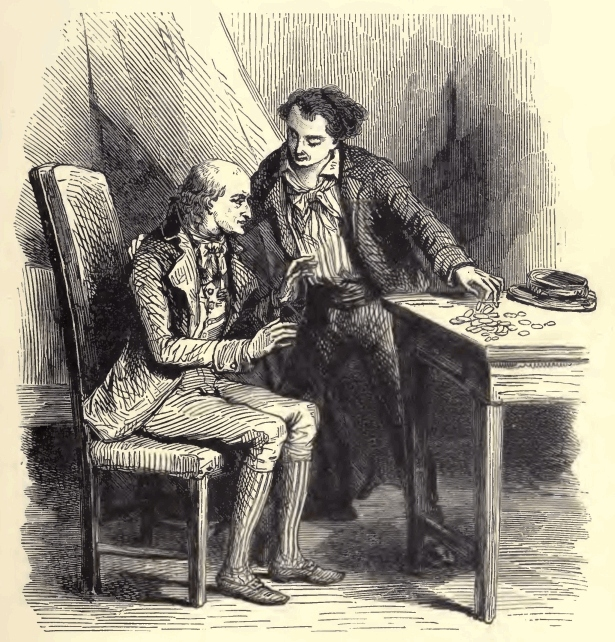
\includegraphics[width=\textwidth]{0035m.jpg}
\end{figure}

“Yes, here I am,” said the young man, “with a promising future and a
little money. Here, father, here!” he said, “take this—take it, and
send for something immediately.” And he emptied his pockets on the
table, the contents consisting of a dozen gold pieces, five or six
five-franc pieces, and some smaller coin. The countenance of old Dantès
brightened.

“Whom does this belong to?” he inquired.

“To me, to you, to us! Take it; buy some provisions; be happy, and
tomorrow we shall have more.”

“Gently, gently,” said the old man, with a smile; “and by your leave I
will use your purse moderately, for they would say, if they saw me buy
too many things at a time, that I had been obliged to await your
return, in order to be able to purchase them.”

“Do as you please; but, first of all, pray have a servant, father. I
will not have you left alone so long. I have some smuggled coffee and
most capital tobacco, in a small chest in the hold, which you shall
have tomorrow. But, hush, here comes somebody.”

“’Tis Caderousse, who has heard of your arrival, and no doubt comes to
congratulate you on your fortunate return.”

“Ah, lips that say one thing, while the heart thinks another,” murmured
Edmond. “But, never mind, he is a neighbor who has done us a service on
a time, so he’s welcome.”

As Edmond paused, the black and bearded head of Caderousse appeared at
the door. He was a man of twenty-five or six, and held a piece of
cloth, which, being a tailor, he was about to make into a coat-lining.

“What, is it you, Edmond, back again?” said he, with a broad
Marseillaise accent, and a grin that displayed his ivory-white teeth.

“Yes, as you see, neighbor Caderousse; and ready to be agreeable to you
in any and every way,” replied Dantès, but ill-concealing his coldness
under this cloak of civility.

“Thanks—thanks; but, fortunately, I do not want for anything; and it
chances that at times there are others who have need of me.” Dantès
made a gesture. “I do not allude to you, my boy. No!—no! I lent you
money, and you returned it; that’s like good neighbors, and we are
quits.”

“We are never quits with those who oblige us,” was Dantès’ reply; “for
when we do not owe them money, we owe them gratitude.”

“What’s the use of mentioning that? What is done is done. Let us talk
of your happy return, my boy. I had gone on the quay to match a piece
of mulberry cloth, when I met friend Danglars. ‘You at
Marseilles?’—‘Yes,’ says he.

“‘I thought you were at Smyrna.’—‘I was; but am now back again.’

“‘And where is the dear boy, our little Edmond?’

“‘Why, with his father, no doubt,’ replied Danglars. And so I came,”
added Caderousse, “as fast as I could to have the pleasure of shaking
hands with a friend.”

\begin{figure}[h]
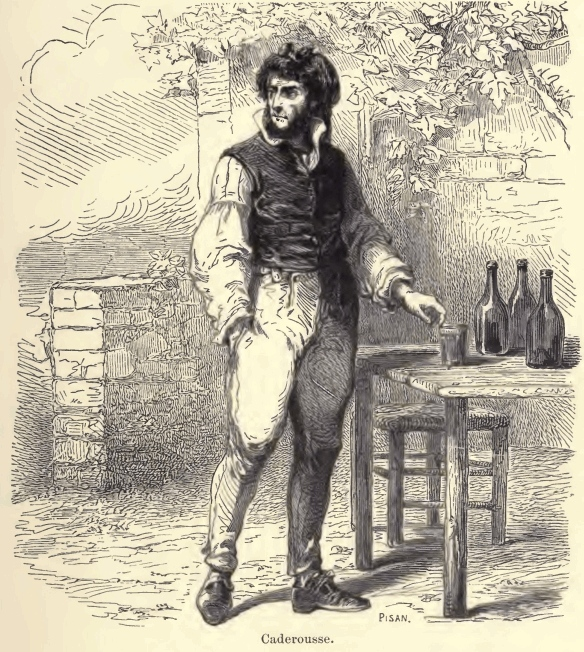
\includegraphics[width=\textwidth]{0037m.jpg}
\end{figure}

“Worthy Caderousse!” said the old man, “he is so much attached to us.”

“Yes, to be sure I am. I love and esteem you, because honest folks are
so rare. But it seems you have come back rich, my boy,” continued the
tailor, looking askance at the handful of gold and silver which Dantès
had thrown on the table.

The young man remarked the greedy glance which shone in the dark eyes
of his neighbor. “Eh,” he said, negligently, “this money is not mine. I
was expressing to my father my fears that he had wanted many things in
my absence, and to convince me he emptied his purse on the table. Come,
father” added Dantès, “put this money back in your box—unless neighbor
Caderousse wants anything, and in that case it is at his service.”

“No, my boy, no,” said Caderousse. “I am not in any want, thank God, my
living is suited to my means. Keep your money—keep it, I say;—one never
has too much;—but, at the same time, my boy, I am as much obliged by
your offer as if I took advantage of it.”

“It was offered with good will,” said Dantès.

“No doubt, my boy; no doubt. Well, you stand well with M. Morrel I
hear,—you insinuating dog, you!”

“M. Morrel has always been exceedingly kind to me,” replied Dantès.

“Then you were wrong to refuse to dine with him.”

“What, did you refuse to dine with him?” said old Dantès; “and did he
invite you to dine?”

“Yes, my dear father,” replied Edmond, smiling at his father’s
astonishment at the excessive honor paid to his son.

“And why did you refuse, my son?” inquired the old man.

“That I might the sooner see you again, my dear father,” replied the
young man. “I was most anxious to see you.”

“But it must have vexed M. Morrel, good, worthy man,” said Caderousse.
“And when you are looking forward to be captain, it was wrong to annoy
the owner.”

“But I explained to him the cause of my refusal,” replied Dantès, “and
I hope he fully understood it.”

“Yes, but to be captain one must do a little flattery to one’s
patrons.”

“I hope to be captain without that,” said Dantès.

“So much the better—so much the better! Nothing will give greater
pleasure to all your old friends; and I know one down there behind the
Saint Nicolas citadel who will not be sorry to hear it.”

“Mercédès?” said the old man.

“Yes, my dear father, and with your permission, now I have seen you,
and know you are well and have all you require, I will ask your consent
to go and pay a visit to the Catalans.”

“Go, my dear boy,” said old Dantès; “and Heaven bless you in your wife,
as it has blessed me in my son!”

“His wife!” said Caderousse; “why, how fast you go on, father Dantès;
she is not his wife yet, as it seems to me.”

“No, but according to all probability she soon will be,” replied
Edmond.

“Yes—yes,” said Caderousse; “but you were right to return as soon as
possible, my boy.”

“And why?”

“Because Mercédès is a very fine girl, and fine girls never lack
followers; she particularly has them by dozens.”

“Really?” answered Edmond, with a smile which had in it traces of
slight uneasiness.

\begin{figure}[h]
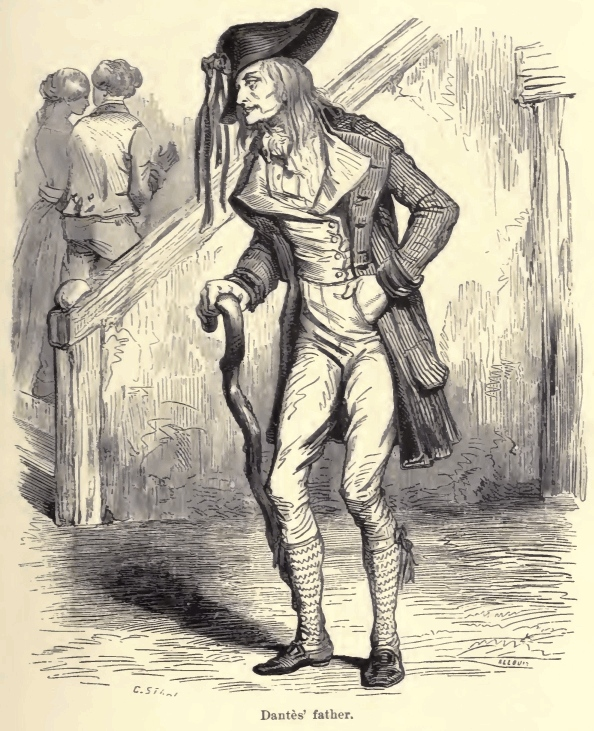
\includegraphics[width=\textwidth]{0039m.jpg}
\end{figure}

“Ah, yes,” continued Caderousse, “and capital offers, too; but you
know, you will be captain, and who could refuse you then?”

“Meaning to say,” replied Dantès, with a smile which but ill-concealed
his trouble, “that if I were not a captain——”

“Eh—eh!” said Caderousse, shaking his head.

“Come, come,” said the sailor, “I have a better opinion than you of
women in general, and of Mercédès in particular; and I am certain that,
captain or not, she will remain ever faithful to me.”

“So much the better—so much the better,” said Caderousse. “When one is
going to be married, there is nothing like implicit confidence; but
never mind that, my boy,—go and announce your arrival, and let her know
all your hopes and prospects.”

“I will go directly,” was Edmond’s reply; and, embracing his father,
and nodding to Caderousse, he left the apartment.

Caderousse lingered for a moment, then taking leave of old Dantès, he
went downstairs to rejoin Danglars, who awaited him at the corner of
the Rue Senac.

“Well,” said Danglars, “did you see him?”

“I have just left him,” answered Caderousse.

“Did he allude to his hope of being captain?”

“He spoke of it as a thing already decided.”

“Indeed!” said Danglars, “he is in too much hurry, it appears to me.”

“Why, it seems M. Morrel has promised him the thing.”

“So that he is quite elated about it?”

“Why, yes, he is actually insolent over the matter—has already offered
me his patronage, as if he were a grand personage, and proffered me a
loan of money, as though he were a banker.”

“Which you refused?”

“Most assuredly; although I might easily have accepted it, for it was I
who put into his hands the first silver he ever earned; but now M.
Dantès has no longer any occasion for assistance—he is about to become
a captain.”

“Pooh!” said Danglars, “he is not one yet.”

“\textit{Ma foi!} it will be as well if he is not,” answered Caderousse; “for
if he should be, there will be really no speaking to him.”

“If we choose,” replied Danglars, “he will remain what he is; and
perhaps become even less than he is.”

“What do you mean?”

“Nothing—I was speaking to myself. And is he still in love with the
Catalane?”

“Over head and ears; but, unless I am much mistaken, there will be a
storm in that quarter.”

\begin{figure}[h]
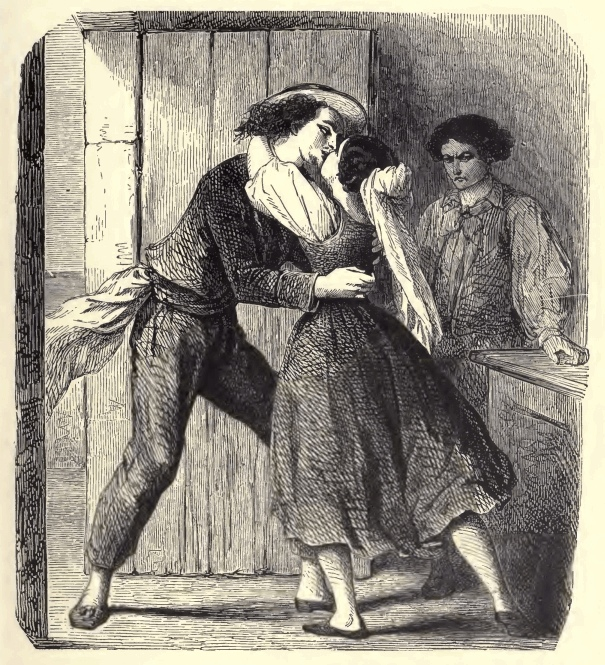
\includegraphics[width=\textwidth]{0041m.jpg}
\end{figure}

“Explain yourself.”

“Why should I?”

“It is more important than you think, perhaps. You do not like Dantès?”

“I never like upstarts.”

“Then tell me all you know about the Catalane.”

“I know nothing for certain; only I have seen things which induce me to
believe, as I told you, that the future captain will find some
annoyance in the vicinity of the Vieilles Infirmeries.”

“What have you seen?—come, tell me!”

“Well, every time I have seen Mercédès come into the city she has been
accompanied by a tall, strapping, black-eyed Catalan, with a red
complexion, brown skin, and fierce air, whom she calls cousin.”

“Really; and you think this cousin pays her attentions?”

“I only suppose so. What else can a strapping chap of twenty-one mean
with a fine wench of seventeen?”

“And you say that Dantès has gone to the Catalans?”

“He went before I came down.”

“Let us go the same way; we will stop at La Réserve, and we can drink a
glass of La Malgue, whilst we wait for news.”

“Come along,” said Caderousse; “but you pay the score.”

“Of course,” replied Danglars; and going quickly to the designated
place, they called for a bottle of wine, and two glasses.

Père Pamphile had seen Dantès pass not ten minutes before; and assured
that he was at the Catalans, they sat down under the budding foliage of
the planes and sycamores, in the branches of which the birds were
singing their welcome to one of the first days of spring.

\printpagenotes*
\chapter{The Catalans}

Beyond a bare, weather-worn wall, about a hundred paces from the spot
where the two friends sat looking and listening as they drank their
wine, was the village of the Catalans. Long ago this mysterious colony
quitted Spain, and settled on the tongue of land on which it is to this
day. Whence it came no one knew, and it spoke an unknown tongue. One of
its chiefs, who understood Provençal, begged the commune of Marseilles
to give them this bare and barren promontory, where, like the sailors
of old, they had run their boats ashore. The request was granted; and
three months afterwards, around the twelve or fifteen small vessels
which had brought these gypsies of the sea, a small village sprang up.
This village, constructed in a singular and picturesque manner, half
Moorish, half Spanish, still remains, and is inhabited by descendants
of the first comers, who speak the language of their fathers. For three
or four centuries they have remained upon this small promontory, on
which they had settled like a flight of seabirds, without mixing with
the Marseillaise population, intermarrying, and preserving their
original customs and the costume of their mother-country as they have
preserved its language.

Our readers will follow us along the only street of this little
village, and enter with us one of the houses, which is sunburned to the
beautiful dead-leaf color peculiar to the buildings of the country, and
within coated with whitewash, like a Spanish posada. A young and
beautiful girl, with hair as black as jet, her eyes as velvety as the
gazelle’s, was leaning with her back against the wainscot, rubbing in
her slender delicately moulded fingers a bunch of heath blossoms, the
flowers of which she was picking off and strewing on the floor; her
arms, bare to the elbow, brown, and modelled after those of the
Arlesian Venus, moved with a kind of restless impatience, and she
tapped the earth with her arched and supple foot, so as to display the
pure and full shape of her well-turned leg, in its red cotton, gray and
blue clocked, stocking. At three paces from her, seated in a chair
which he balanced on two legs, leaning his elbow on an old worm-eaten
table, was a tall young man of twenty, or two-and-twenty, who was
looking at her with an air in which vexation and uneasiness were
mingled. He questioned her with his eyes, but the firm and steady gaze
of the young girl controlled his look.

“You see, Mercédès,” said the young man, “here is Easter come round
again; tell me, is this the moment for a wedding?”

“I have answered you a hundred times, Fernand, and really you must be
very stupid to ask me again.”

“Well, repeat it,—repeat it, I beg of you, that I may at last believe
it! Tell me for the hundredth time that you refuse my love, which had
your mother’s sanction. Make me understand once for all that you are
trifling with my happiness, that my life or death are nothing to you.
Ah, to have dreamed for ten years of being your husband, Mercédès, and
to lose that hope, which was the only stay of my existence!”

“At least it was not I who ever encouraged you in that hope, Fernand,”
replied Mercédès; “you cannot reproach me with the slightest coquetry.
I have always said to you, ‘I love you as a brother; but do not ask
from me more than sisterly affection, for my heart is another’s.’ Is
not this true, Fernand?”

“Yes, that is very true, Mercédès,” replied the young man, “Yes, you
have been cruelly frank with me; but do you forget that it is among the
Catalans a sacred law to intermarry?”

\begin{figure}[ht]
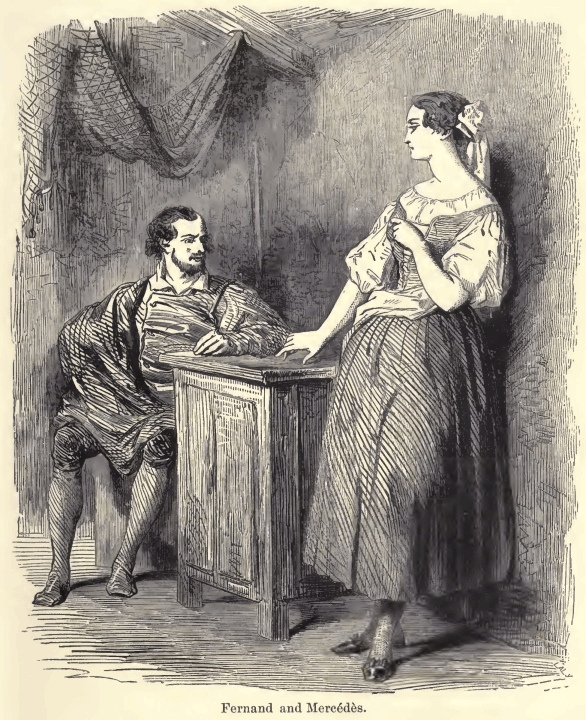
\includegraphics[width=\textwidth]{0045m.jpg}
\end{figure}

“You mistake, Fernand; it is not a law, but merely a custom, and, I
pray of you, do not cite this custom in your favor. You are included in
the conscription, Fernand, and are only at liberty on sufferance,
liable at any moment to be called upon to take up arms. Once a soldier,
what would you do with me, a poor orphan, forlorn, without fortune,
with nothing but a half-ruined hut and a few ragged nets, the miserable
inheritance left by my father to my mother, and by my mother to me? She
has been dead a year, and you know, Fernand, I have subsisted almost
entirely on public charity. Sometimes you pretend I am useful to you,
and that is an excuse to share with me the produce of your fishing, and
I accept it, Fernand, because you are the son of my father’s brother,
because we were brought up together, and still more because it would
give you so much pain if I refuse. But I feel very deeply that this
fish which I go and sell, and with the produce of which I buy the flax
I spin,—I feel very keenly, Fernand, that this is charity.”

“And if it were, Mercédès, poor and lone as you are, you suit me as
well as the daughter of the first shipowner or the richest banker of
Marseilles! What do such as we desire but a good wife and careful
housekeeper, and where can I look for these better than in you?”

“Fernand,” answered Mercédès, shaking her head, “a woman becomes a bad
manager, and who shall say she will remain an honest woman, when she
loves another man better than her husband? Rest content with my
friendship, for I say once more that is all I can promise, and I will
promise no more than I can bestow.”

“I understand,” replied Fernand, “you can endure your own wretchedness
patiently, but you are afraid to share mine. Well, Mercédès, beloved by
you, I would tempt fortune; you would bring me good luck, and I should
become rich. I could extend my occupation as a fisherman, might get a
place as clerk in a warehouse, and become in time a dealer myself.”

“You could do no such thing, Fernand; you are a soldier, and if you
remain at the Catalans it is because there is no war; so remain a
fisherman, and contented with my friendship, as I cannot give you
more.”

“Well, I will do better, Mercédès. I will be a sailor; instead of the
costume of our fathers, which you despise, I will wear a varnished hat,
a striped shirt, and a blue jacket, with an anchor on the buttons.
Would not that dress please you?”

“What do you mean?” asked Mercédès, with an angry glance,—“what do you
mean? I do not understand you?”

“I mean, Mercédès, that you are thus harsh and cruel with me, because
you are expecting someone who is thus attired; but perhaps he whom you
await is inconstant, or if he is not, the sea is so to him.”

“Fernand,” cried Mercédès, “I believed you were good-hearted, and I was
mistaken! Fernand, you are wicked to call to your aid jealousy and the
anger of God! Yes, I will not deny it, I do await, and I do love him of
whom you speak; and, if he does not return, instead of accusing him of
the inconstancy which you insinuate, I will tell you that he died
loving me and me only.” The young girl made a gesture of rage. “I
understand you, Fernand; you would be revenged on him because I do not
love you; you would cross your Catalan knife with his dirk. What end
would that answer? To lose you my friendship if he were conquered, and
see that friendship changed into hate if you were victor. Believe me,
to seek a quarrel with a man is a bad method of pleasing the woman who
loves that man. No, Fernand, you will not thus give way to evil
thoughts. Unable to have me for your wife, you will content yourself
with having me for your friend and sister; and besides,” she added, her
eyes troubled and moistened with tears, “wait, wait, Fernand; you said
just now that the sea was treacherous, and he has been gone four
months, and during these four months there have been some terrible
storms.”

Fernand made no reply, nor did he attempt to check the tears which
flowed down the cheeks of Mercédès, although for each of these tears he
would have shed his heart’s blood; but these tears flowed for another.
He arose, paced a while up and down the hut, and then, suddenly
stopping before Mercédès, with his eyes glowing and his hands
clenched,—“Say, Mercédès,” he said, “once for all, is this your final
determination?”

“I love Edmond Dantès,” the young girl calmly replied, “and none but
Edmond shall ever be my husband.”

“And you will always love him?”

“As long as I live.”

Fernand let fall his head like a defeated man, heaved a sigh that was
like a groan, and then suddenly looking her full in the face, with
clenched teeth and expanded nostrils, said,—“But if he is dead——”

“If he is dead, I shall die too.”

“If he has forgotten you——”

“Mercédès!” called a joyous voice from without,—“Mercédès!”

“Ah,” exclaimed the young girl, blushing with delight, and fairly
leaping in excess of love, “you see he has not forgotten me, for here
he is!” And rushing towards the door, she opened it, saying, “Here,
Edmond, here I am!”

Fernand, pale and trembling, drew back, like a traveller at the sight
of a serpent, and fell into a chair beside him. Edmond and Mercédès
were clasped in each other’s arms. The burning Marseilles sun, which
shot into the room through the open door, covered them with a flood of
light. At first they saw nothing around them. Their intense happiness
isolated them from all the rest of the world, and they only spoke in
broken words, which are the tokens of a joy so extreme that they seem
rather the expression of sorrow. Suddenly Edmond saw the gloomy, pale,
and threatening countenance of Fernand, as it was defined in the
shadow. By a movement for which he could scarcely account to himself,
the young Catalan placed his hand on the knife at his belt.

“Ah, your pardon,” said Dantès, frowning in his turn; “I did not
perceive that there were three of us.” Then, turning to Mercédès, he
inquired, “Who is this gentleman?”

“One who will be your best friend, Dantès, for he is my friend, my
cousin, my brother; it is Fernand—the man whom, after you, Edmond, I
love the best in the world. Do you not remember him?”

“Yes!” said Dantès, and without relinquishing Mercédès’ hand clasped in
one of his own, he extended the other to the Catalan with a cordial
air. But Fernand, instead of responding to this amiable gesture,
remained mute and trembling. Edmond then cast his eyes scrutinizingly
at the agitated and embarrassed Mercédès, and then again on the gloomy
and menacing Fernand. This look told him all, and his anger waxed hot.

“I did not know, when I came with such haste to you, that I was to meet
an enemy here.”

“An enemy!” cried Mercédès, with an angry look at her cousin. “An enemy
in my house, do you say, Edmond! If I believed that, I would place my
arm under yours and go with you to Marseilles, leaving the house to
return to it no more.”

Fernand’s eye darted lightning. “And should any misfortune occur to
you, dear Edmond,” she continued with the same calmness which proved to
Fernand that the young girl had read the very innermost depths of his
sinister thought, “if misfortune should occur to you, I would ascend
the highest point of the Cape de Morgiou and cast myself headlong from
it.”

Fernand became deadly pale. “But you are deceived, Edmond,” she
continued. “You have no enemy here—there is no one but Fernand, my
brother, who will grasp your hand as a devoted friend.”

And at these words the young girl fixed her imperious look on the
Catalan, who, as if fascinated by it, came slowly towards Edmond, and
offered him his hand. His hatred, like a powerless though furious wave,
was broken against the strong ascendancy which Mercédès exercised over
him. Scarcely, however, had he touched Edmond’s hand when he felt he
had done all he could do, and rushed hastily out of the house.

“Oh,” he exclaimed, running furiously and tearing his hair—“Oh, who
will deliver me from this man? Wretched—wretched that I am!”

“Hallo, Catalan! Hallo, Fernand! where are you running to?” exclaimed a
voice.

The young man stopped suddenly, looked around him, and perceived
Caderousse sitting at table with Danglars, under an arbor.

“Well”, said Caderousse, “why don’t you come? Are you really in such a
hurry that you have no time to pass the time of day with your friends?”

“Particularly when they have still a full bottle before them,” added
Danglars. Fernand looked at them both with a stupefied air, but did not
say a word.

“He seems besotted,” said Danglars, pushing Caderousse with his knee.
“Are we mistaken, and is Dantès triumphant in spite of all we have
believed?”

“Why, we must inquire into that,” was Caderousse’s reply; and turning
towards the young man, said, “Well, Catalan, can’t you make up your
mind?”

Fernand wiped away the perspiration steaming from his brow, and slowly
entered the arbor, whose shade seemed to restore somewhat of calmness
to his senses, and whose coolness somewhat of refreshment to his
exhausted body.

“Good-day,” said he. “You called me, didn’t you?” And he fell, rather
than sat down, on one of the seats which surrounded the table.

“I called you because you were running like a madman, and I was afraid
you would throw yourself into the sea,” said Caderousse, laughing.
“Why, when a man has friends, they are not only to offer him a glass of
wine, but, moreover, to prevent his swallowing three or four pints of
water unnecessarily!”

Fernand gave a groan, which resembled a sob, and dropped his head into
his hands, his elbows leaning on the table.

“Well, Fernand, I must say,” said Caderousse, beginning the
conversation, with that brutality of the common people in which
curiosity destroys all diplomacy, “you look uncommonly like a rejected
lover;” and he burst into a hoarse laugh.

“Bah!” said Danglars, “a lad of his make was not born to be unhappy in
love. You are laughing at him, Caderousse.”

“No,” he replied, “only hark how he sighs! Come, come, Fernand,” said
Caderousse, “hold up your head, and answer us. It’s not polite not to
reply to friends who ask news of your health.”

“My health is well enough,” said Fernand, clenching his hands without
raising his head.

“Ah, you see, Danglars,” said Caderousse, winking at his friend, “this
is how it is; Fernand, whom you see here, is a good and brave Catalan,
one of the best fishermen in Marseilles, and he is in love with a very
fine girl, named Mercédès; but it appears, unfortunately, that the fine
girl is in love with the mate of the \textit{Pharaon}; and as the \textit{Pharaon}
arrived today—why, you understand!”

“No; I do not understand,” said Danglars.

“Poor Fernand has been dismissed,” continued Caderousse.

“Well, and what then?” said Fernand, lifting up his head, and looking
at Caderousse like a man who looks for someone on whom to vent his
anger; “Mercédès is not accountable to any person, is she? Is she not
free to love whomsoever she will?”

“Oh, if you take it in that sense,” said Caderousse, “it is another
thing. But I thought you were a Catalan, and they told me the Catalans
were not men to allow themselves to be supplanted by a rival. It was
even told me that Fernand, especially, was terrible in his vengeance.”

Fernand smiled piteously. “A lover is never terrible,” he said.

“Poor fellow!” remarked Danglars, affecting to pity the young man from
the bottom of his heart. “Why, you see, he did not expect to see Dantès
return so suddenly—he thought he was dead, perhaps; or perchance
faithless! These things always come on us more severely when they come
suddenly.”

“Ah, \textit{ma foi}, under any circumstances!” said Caderousse, who drank as
he spoke, and on whom the fumes of the wine began to take
effect,—“under any circumstances Fernand is not the only person put out
by the fortunate arrival of Dantès; is he, Danglars?”

“No, you are right—and I should say that would bring him ill-luck.”

“Well, never mind,” answered Caderousse, pouring out a glass of wine
for Fernand, and filling his own for the eighth or ninth time, while
Danglars had merely sipped his. “Never mind—in the meantime he marries
Mercédès—the lovely Mercédès—at least he returns to do that.”

During this time Danglars fixed his piercing glance on the young man,
on whose heart Caderousse’s words fell like molten lead.

“And when is the wedding to be?” he asked.

“Oh, it is not yet fixed!” murmured Fernand.

“No, but it will be,” said Caderousse, “as surely as Dantès will be
captain of the \textit{Pharaon}—eh, Danglars?”

Danglars shuddered at this unexpected attack, and turned to Caderousse,
whose countenance he scrutinized, to try and detect whether the blow
was premeditated; but he read nothing but envy in a countenance already
rendered brutal and stupid by drunkenness.

“Well,” said he, filling the glasses, “let us drink to Captain Edmond
Dantès, husband of the beautiful Catalane!”

Caderousse raised his glass to his mouth with unsteady hand, and
swallowed the contents at a gulp. Fernand dashed his on the ground.

“Eh, eh, eh!” stammered Caderousse. “What do I see down there by the
wall, in the direction of the Catalans? Look, Fernand, your eyes are
better than mine. I believe I see double. You know wine is a deceiver;
but I should say it was two lovers walking side by side, and hand in
hand. Heaven forgive me, they do not know that we can see them, and
they are actually embracing!”

Danglars did not lose one pang that Fernand endured.

“Do you know them, Fernand?” he said.

“Yes,” was the reply, in a low voice. “It is Edmond and Mercédès!”

“Ah, see there, now!” said Caderousse; “and I did not recognize them!
Hallo, Dantès! hello, lovely damsel! Come this way, and let us know
when the wedding is to be, for Fernand here is so obstinate he will not
tell us.”

“Hold your tongue, will you?” said Danglars, pretending to restrain
Caderousse, who, with the tenacity of drunkards, leaned out of the
arbor. “Try to stand upright, and let the lovers make love without
interruption. See, look at Fernand, and follow his example; he is
well-behaved!”

\begin{figure}[h]
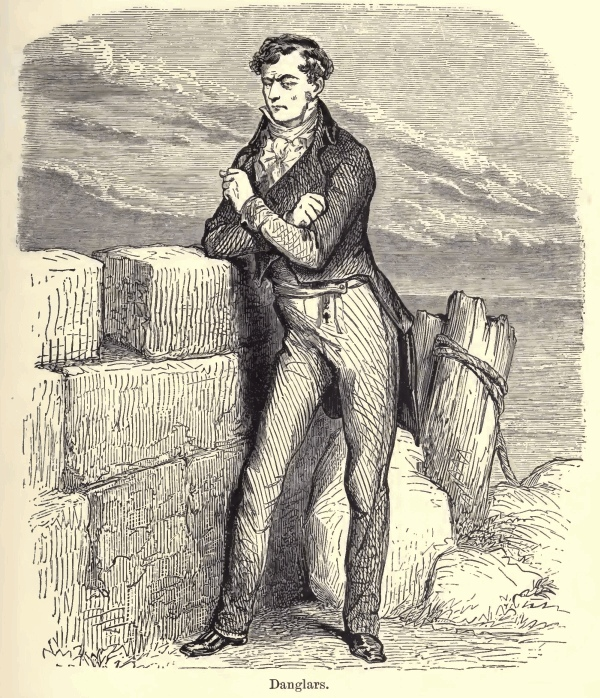
\includegraphics[width=\textwidth]{0051m.jpg}
\end{figure}

Fernand, probably excited beyond bearing, pricked by Danglars, as the
bull is by the bandilleros, was about to rush out; for he had risen
from his seat, and seemed to be collecting himself to dash headlong
upon his rival, when Mercédès, smiling and graceful, lifted up her
lovely head, and looked at them with her clear and bright eyes. At this
Fernand recollected her threat of dying if Edmond died, and dropped
again heavily on his seat. Danglars looked at the two men, one after
the other, the one brutalized by liquor, the other overwhelmed with
love.

“I shall get nothing from these fools,” he muttered; “and I am very
much afraid of being here between a drunkard and a coward. Here’s an
envious fellow making himself boozy on wine when he ought to be nursing
his wrath, and here is a fool who sees the woman he loves stolen from
under his nose and takes on like a big baby. Yet this Catalan has eyes
that glisten like those of the vengeful Spaniards, Sicilians, and
Calabrians, and the other has fists big enough to crush an ox at one
blow. Unquestionably, Edmond’s star is in the ascendant, and he will
marry the splendid girl—he will be captain, too, and laugh at us all,
unless”—a sinister smile passed over Danglars’ lips—“unless I take a
hand in the affair,” he added.

“Hallo!” continued Caderousse, half-rising, and with his fist on the
table, “hallo, Edmond! do you not see your friends, or are you too
proud to speak to them?”

“No, my dear fellow!” replied Dantès, “I am not proud, but I am happy,
and happiness blinds, I think, more than pride.”

“Ah, very well, that’s an explanation!” said Caderousse. “How do you
do, Madame Dantès?”

Mercédès courtesied gravely, and said—“That is not my name, and in my
country it bodes ill fortune, they say, to call a young girl by the
name of her betrothed before he becomes her husband. So call me
Mercédès, if you please.”

“We must excuse our worthy neighbor, Caderousse,” said Dantès, “he is
so easily mistaken.”

“So, then, the wedding is to take place immediately, M. Dantès,” said
Danglars, bowing to the young couple.

“As soon as possible, M. Danglars; today all preliminaries will be
arranged at my father’s, and tomorrow, or next day at latest, the
wedding festival here at La Réserve. My friends will be there, I hope;
that is to say, you are invited, M. Danglars, and you, Caderousse.”

“And Fernand,” said Caderousse with a chuckle; “Fernand, too, is
invited!”

“My wife’s brother is my brother,” said Edmond; “and we, Mercédès and
I, should be very sorry if he were absent at such a time.”

Fernand opened his mouth to reply, but his voice died on his lips, and
he could not utter a word.

“Today the preliminaries, tomorrow or next day the ceremony! You are in
a hurry, captain!”

“Danglars,” said Edmond, smiling, “I will say to you as Mercédès said
just now to Caderousse, ‘Do not give me a title which does not belong
to me’; that may bring me bad luck.”

“Your pardon,” replied Danglars, “I merely said you seemed in a hurry,
and we have lots of time; the \textit{Pharaon} cannot be under weigh again in
less than three months.”

“We are always in a hurry to be happy, M. Danglars; for when we have
suffered a long time, we have great difficulty in believing in good
fortune. But it is not selfishness alone that makes me thus in haste; I
must go to Paris.”

“Ah, really?—to Paris! and will it be the first time you have ever been
there, Dantès?”

“Yes.”

“Have you business there?”

“Not of my own; the last commission of poor Captain Leclere; you know
to what I allude, Danglars—it is sacred. Besides, I shall only take the
time to go and return.”

“Yes, yes, I understand,” said Danglars, and then in a low tone, he
added, “To Paris, no doubt to deliver the letter which the grand
marshal gave him. Ah, this letter gives me an idea—a capital idea! Ah;
Dantès, my friend, you are not yet registered number one on board the
good ship \textit{Pharaon};” then turning towards Edmond, who was walking
away, “A pleasant journey,” he cried.

“Thank you,” said Edmond with a friendly nod, and the two lovers
continued on their way, as calm and joyous as if they were the very
elect of heaven.

\printpagenotes*
\chapter{Conspiracy}

Danglars followed Edmond and Mercédès with his eyes until the two
lovers disappeared behind one of the angles of Fort Saint Nicolas;
then, turning round, he perceived Fernand, who had fallen, pale and
trembling, into his chair, while Caderousse stammered out the words of
a drinking-song.

“Well, my dear sir,” said Danglars to Fernand, “here is a marriage
which does not appear to make everybody happy.”

“It drives me to despair,” said Fernand.

“Do you, then, love Mercédès?”

“I adore her!”

“For long?”

“As long as I have known her—always.”

“And you sit there, tearing your hair, instead of seeking to remedy
your condition; I did not think that was the way of your people.”

“What would you have me do?” said Fernand.

“How do I know? Is it my affair? I am not in love with Mademoiselle
Mercédès; but for you—in the words of the gospel, seek, and you shall
find.”

“I have found already.”

“What?”

“I would stab the man, but the woman told me that if any misfortune
happened to her betrothed, she would kill herself.”

“Pooh! Women say those things, but never do them.”

“You do not know Mercédès; what she threatens she will do.”

“Idiot!” muttered Danglars; “whether she kill herself or not, what
matter, provided Dantès is not captain?”

“Before Mercédès should die,” replied Fernand, with the accents of
unshaken resolution, “I would die myself!”

“That’s what I call love!” said Caderousse with a voice more tipsy than
ever. “That’s love, or I don’t know what love is.”

“Come,” said Danglars, “you appear to me a good sort of fellow, and
hang me, I should like to help you, but——”

“Yes,” said Caderousse, “but how?”

“My dear fellow,” replied Danglars, “you are three parts drunk; finish
the bottle, and you will be completely so. Drink then, and do not
meddle with what we are discussing, for that requires all one’s wit and
cool judgment.”

“I—drunk!” said Caderousse; “well that’s a good one! I could drink four
more such bottles; they are no bigger than cologne flasks. Père
Pamphile, more wine!”

And Caderousse rattled his glass upon the table.

“You were saying, sir——” said Fernand, awaiting with great anxiety the
end of this interrupted remark.

“What was I saying? I forget. This drunken Caderousse has made me lose
the thread of my sentence.”

“Drunk, if you like; so much the worse for those who fear wine, for it
is because they have bad thoughts which they are afraid the liquor will
extract from their hearts;” and Caderousse began to sing the two last
lines of a song very popular at the time:

\hspace{1cm}{\small ‘Tous les méchants sont buveurs d’eau;

\hspace{1cm}C’est bien prouvé par le déluge.’}\footnote[1]{“The wicked
are great drinkers of water; As the flood proved once for all.” }

“You said, sir, you would like to help me, but——”

“Yes; but I added, to help you it would be sufficient that Dantès did
not marry her you love; and the marriage may easily be thwarted,
methinks, and yet Dantès need not die.”

“Death alone can separate them,” remarked Fernand.

“You talk like a noodle, my friend,” said Caderousse; “and here is
Danglars, who is a wide-awake, clever, deep fellow, who will prove to
you that you are wrong. Prove it, Danglars. I have answered for you.
Say there is no need why Dantès should die; it would, indeed, be a pity
he should. Dantès is a good fellow; I like Dantès. Dantès, your
health.”

Fernand rose impatiently. “Let him run on,” said Danglars, restraining
the young man; “drunk as he is, he is not much out in what he says.
Absence severs as well as death, and if the walls of a prison were
between Edmond and Mercédès they would be as effectually separated as
if he lay under a tombstone.”

\begin{figure}[ht]
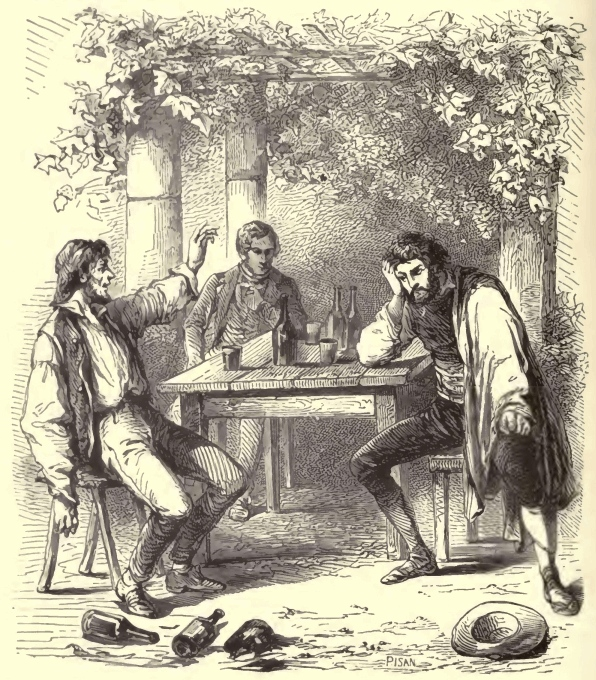
\includegraphics[width=\textwidth]{0056m.jpg}
\end{figure}

“Yes; but one gets out of prison,” said Caderousse, who, with what
sense was left him, listened eagerly to the conversation, “and when one
gets out and one’s name is Edmond Dantès, one seeks revenge——”

“What matters that?” muttered Fernand.

“And why, I should like to know,” persisted Caderousse, “should they
put Dantès in prison? he has neither robbed, nor killed, nor murdered.”

“Hold your tongue!” said Danglars.

“I won’t hold my tongue!” replied Caderousse; “I say I want to know why
they should put Dantès in prison; I like Dantès; Dantès, your health!”
and he swallowed another glass of wine.

\begin{figure}[ht]
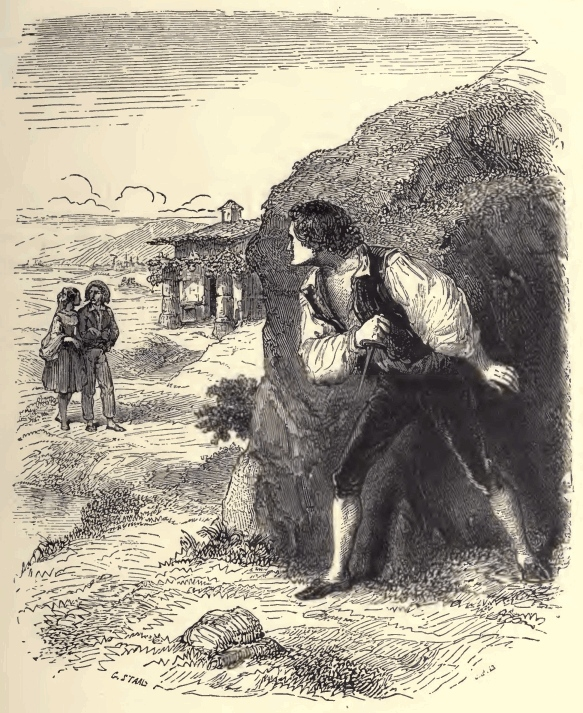
\includegraphics[width=\textwidth]{0057m.jpg}
\end{figure}

Danglars saw in the muddled look of the tailor the progress of his
intoxication, and turning towards Fernand, said, “Well, you understand
there is no need to kill him.”

“Certainly not, if, as you said just now, you have the means of having
Dantès arrested. Have you that means?”

“It is to be found for the searching. But why should I meddle in the
matter? it is no affair of mine.”

“I know not why you meddle,” said Fernand, seizing his arm; “but this I
know, you have some motive of personal hatred against Dantès, for he
who himself hates is never mistaken in the sentiments of others.”

“I! motives of hatred against Dantès? None, on my word! I saw you were
unhappy, and your unhappiness interested me; that’s all; but since you
believe I act for my own account, adieu, my dear friend, get out of the
affair as best you may;” and Danglars rose as if he meant to depart.

“No, no,” said Fernand, restraining him, “stay! It is of very little
consequence to me at the end of the matter whether you have any angry
feeling or not against Dantès. I hate him! I confess it openly. Do you
find the means, I will execute it, provided it is not to kill the man,
for Mercédès has declared she will kill herself if Dantès is killed.”

Caderousse, who had let his head drop on the table, now raised it, and
looking at Fernand with his dull and fishy eyes, he said, “Kill Dantès!
who talks of killing Dantès? I won’t have him killed—I won’t! He’s my
friend, and this morning offered to share his money with me, as I
shared mine with him. I won’t have Dantès killed—I won’t!”

“And who has said a word about killing him, muddlehead?” replied
Danglars. “We were merely joking; drink to his health,” he added,
filling Caderousse’s glass, “and do not interfere with us.”

“Yes, yes, Dantès’ good health!” said Caderousse, emptying his glass,
“here’s to his health! his health—hurrah!”

“But the means—the means?” said Fernand.

“Have you not hit upon any?” asked Danglars.

“No!—you undertook to do so.”

“True,” replied Danglars; “the French have the superiority over the
Spaniards, that the Spaniards ruminate, while the French invent.”

“Do you invent, then,” said Fernand impatiently.

“Waiter,” said Danglars, “pen, ink, and paper.”

“Pen, ink, and paper,” muttered Fernand.

“Yes; I am a supercargo; pen, ink, and paper are my tools, and without
my tools I am fit for nothing.”

“Pen, ink, and paper, then,” called Fernand loudly.

“There’s what you want on that table,” said the waiter.

“Bring them here.” The waiter did as he was desired.

\begin{figure}[h]
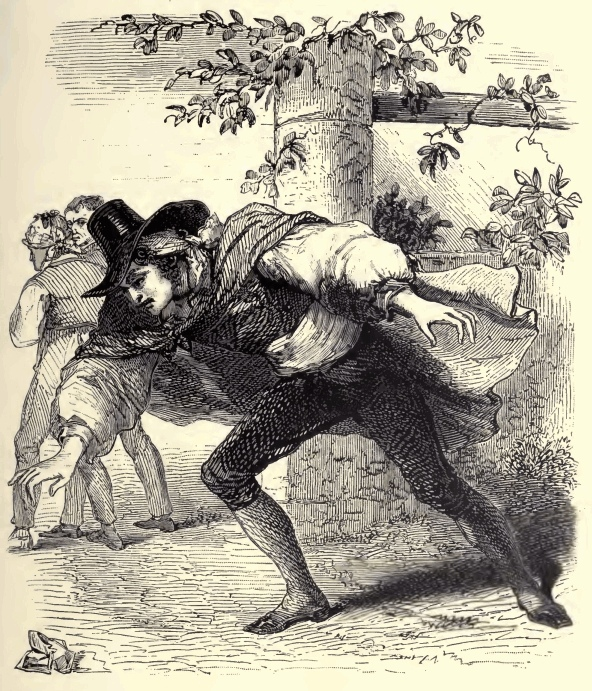
\includegraphics[width=\textwidth]{0059m.jpg}
\end{figure}

“When one thinks,” said Caderousse, letting his hand drop on the paper,
“there is here wherewithal to kill a man more sure than if we waited at
the corner of a wood to assassinate him! I have always had more dread
of a pen, a bottle of ink, and a sheet of paper, than of a sword or
pistol.”

“The fellow is not so drunk as he appears to be,” said Danglars. “Give
him some more wine, Fernand.” Fernand filled Caderousse’s glass, who,
like the confirmed toper he was, lifted his hand from the paper and
seized the glass.

The Catalan watched him until Caderousse, almost overcome by this fresh
assault on his senses, rested, or rather dropped, his glass upon the
table.

“Well!” resumed the Catalan, as he saw the final glimmer of
Caderousse’s reason vanishing before the last glass of wine.

“Well, then, I should say, for instance,” resumed Danglars, “that if
after a voyage such as Dantès has just made, in which he touched at the
Island of Elba, someone were to denounce him to the king’s procureur as
a Bonapartist agent——”

“I will denounce him!” exclaimed the young man hastily.

“Yes, but they will make you then sign your declaration, and confront
you with him you have denounced; I will supply you with the means of
supporting your accusation, for I know the fact well. But Dantès cannot
remain forever in prison, and one day or other he will leave it, and
the day when he comes out, woe betide him who was the cause of his
incarceration!”

“Oh, I should wish nothing better than that he would come and seek a
quarrel with me.”

“Yes, and Mercédès! Mercédès, who will detest you if you have only the
misfortune to scratch the skin of her dearly beloved Edmond!”

“True!” said Fernand.

“No, no,” continued Danglars; “if we resolve on such a step, it would
be much better to take, as I now do, this pen, dip it into this ink,
and write with the left hand (that the writing may not be recognized)
the denunciation we propose.” And Danglars, uniting practice with
theory, wrote with his left hand, and in a writing reversed from his
usual style, and totally unlike it, the following lines, which he
handed to Fernand, and which Fernand read in an undertone:

“The honorable, the king’s attorney, is informed by a friend of the
throne and religion, that one Edmond Dantès, mate of the ship
\textit{Pharaon}, arrived this morning from Smyrna, after having touched at
Naples and Porto-Ferrajo, has been intrusted by Murat with a letter for
the usurper, and by the usurper with a letter for the Bonapartist
committee in Paris. Proof of this crime will be found on arresting him,
for the letter will be found upon him, or at his father’s, or in his
cabin on board the \textit{Pharaon}.”

“Very good,” resumed Danglars; “now your revenge looks like common
sense, for in no way can it revert to yourself, and the matter will
thus work its own way; there is nothing to do now but fold the letter
as I am doing, and write upon it, ‘To the king’s attorney,’ and that’s
all settled.” And Danglars wrote the address as he spoke.

“Yes, and that’s all settled!” exclaimed Caderousse, who, by a last
effort of intellect, had followed the reading of the letter, and
instinctively comprehended all the misery which such a denunciation
must entail. “Yes, and that’s all settled; only it will be an infamous
shame;” and he stretched out his hand to reach the letter.

“Yes,” said Danglars, taking it from beyond his reach; “and as what I
say and do is merely in jest, and I, amongst the first and foremost,
should be sorry if anything happened to Dantès—the worthy Dantès—look
here!” And taking the letter, he squeezed it up in his hands and threw
it into a corner of the arbor.

“All right!” said Caderousse. “Dantès is my friend, and I won’t have
him ill-used.”

“And who thinks of using him ill? Certainly neither I nor Fernand,”
said Danglars, rising and looking at the young man, who still remained
seated, but whose eye was fixed on the denunciatory sheet of paper
flung into the corner.

“In this case,” replied Caderousse, “let’s have some more wine. I wish
to drink to the health of Edmond and the lovely Mercédès.”

“You have had too much already, drunkard,” said Danglars; “and if you
continue, you will be compelled to sleep here, because unable to stand
on your legs.”

“I?” said Caderousse, rising with all the offended dignity of a drunken
man, “I can’t keep on my legs? Why, I’ll wager I can go up into the
belfry of the Accoules, and without staggering, too!”

“Done!” said Danglars, “I’ll take your bet; but tomorrow—today it is
time to return. Give me your arm, and let us go.”

“Very well, let us go,” said Caderousse; “but I don’t want your arm at
all. Come, Fernand, won’t you return to Marseilles with us?”

“No,” said Fernand; “I shall return to the Catalans.”

“You’re wrong. Come with us to Marseilles—come along.”

“I will not.”

“What do you mean? you will not? Well, just as you like, my prince;
there’s liberty for all the world. Come along, Danglars, and let the
young gentleman return to the Catalans if he chooses.”

Danglars took advantage of Caderousse’s temper at the moment, to take
him off towards Marseilles by the Porte Saint-Victor, staggering as he
went.

When they had advanced about twenty yards, Danglars looked back and saw
Fernand stoop, pick up the crumpled paper, and putting it into his
pocket then rush out of the arbor towards Pillon.

“Well,” said Caderousse, “why, what a lie he told! He said he was going
to the Catalans, and he is going to the city. Hallo, Fernand! You are
coming, my boy!”

“Oh, you don’t see straight,” said Danglars; “he’s gone right by the
road to the Vieilles Infirmeries.”

“Well,” said Caderousse, “I should have sworn that he turned to the
right—how treacherous wine is!”

“Come, come,” said Danglars to himself, “now the thing is at work and
it will effect its purpose unassisted.”

\printpagenotes*
\chapter{The Marriage Feast}

The morning’s sun rose clear and resplendent, touching the foamy waves
into a network of ruby-tinted light.

The feast had been made ready on the second floor at La Réserve, with
whose arbor the reader is already familiar. The apartment destined for
the purpose was spacious and lighted by a number of windows, over each
of which was written in golden letters for some inexplicable reason the
name of one of the principal cities of France; beneath these windows a
wooden balcony extended the entire length of the house. And although
the entertainment was fixed for twelve o’clock, an hour previous to
that time the balcony was filled with impatient and expectant guests,
consisting of the favored part of the crew of the \textit{Pharaon}, and other
personal friends of the bridegroom, the whole of whom had arrayed
themselves in their choicest costumes, in order to do greater honor to
the occasion.

Various rumors were afloat to the effect that the owners of the
\textit{Pharaon} had promised to attend the nuptial feast; but all seemed
unanimous in doubting that an act of such rare and exceeding
condescension could possibly be intended.

Danglars, however, who now made his appearance, accompanied by
Caderousse, effectually confirmed the report, stating that he had
recently conversed with M. Morrel, who had himself assured him of his
intention to dine at La Réserve.

In fact, a moment later M. Morrel appeared and was saluted with an
enthusiastic burst of applause from the crew of the \textit{Pharaon}, who
hailed the visit of the shipowner as a sure indication that the man
whose wedding feast he thus delighted to honor would ere long be first
in command of the ship; and as Dantès was universally beloved on board
his vessel, the sailors put no restraint on their tumultuous joy at
finding that the opinion and choice of their superiors so exactly
coincided with their own.

With the entrance of M. Morrel, Danglars and Caderousse were despatched
in search of the bridegroom to convey to him the intelligence of the
arrival of the important personage whose coming had created such a
lively sensation, and to beseech him to make haste.

Danglars and Caderousse set off upon their errand at full speed; but
ere they had gone many steps they perceived a group advancing towards
them, composed of the betrothed pair, a party of young girls in
attendance on the bride, by whose side walked Dantès’ father; the whole
brought up by Fernand, whose lips wore their usual sinister smile.

Neither Mercédès nor Edmond observed the strange expression of his
countenance; they were so happy that they were conscious only of the
sunshine and the presence of each other.

Having acquitted themselves of their errand, and exchanged a hearty
shake of the hand with Edmond, Danglars and Caderousse took their
places beside Fernand and old Dantès,—the latter of whom attracted
universal notice.

The old man was attired in a suit of glistening watered silk, trimmed
with steel buttons, beautifully cut and polished. His thin but wiry
legs were arrayed in a pair of richly embroidered clocked stockings,
evidently of English manufacture, while from his three-cornered hat
depended a long streaming knot of white and blue ribbons. Thus he came
along, supporting himself on a curiously carved stick, his aged
countenance lit up with happiness, looking for all the world like one
of the aged dandies of 1796, parading the newly opened gardens of the
Luxembourg and Tuileries.

Beside him glided Caderousse, whose desire to partake of the good
things provided for the wedding party had induced him to become
reconciled to the Dantès, father and son, although there still lingered
in his mind a faint and unperfect recollection of the events of the
preceding night; just as the brain retains on waking in the morning the
dim and misty outline of a dream.

\begin{figure}[ht]
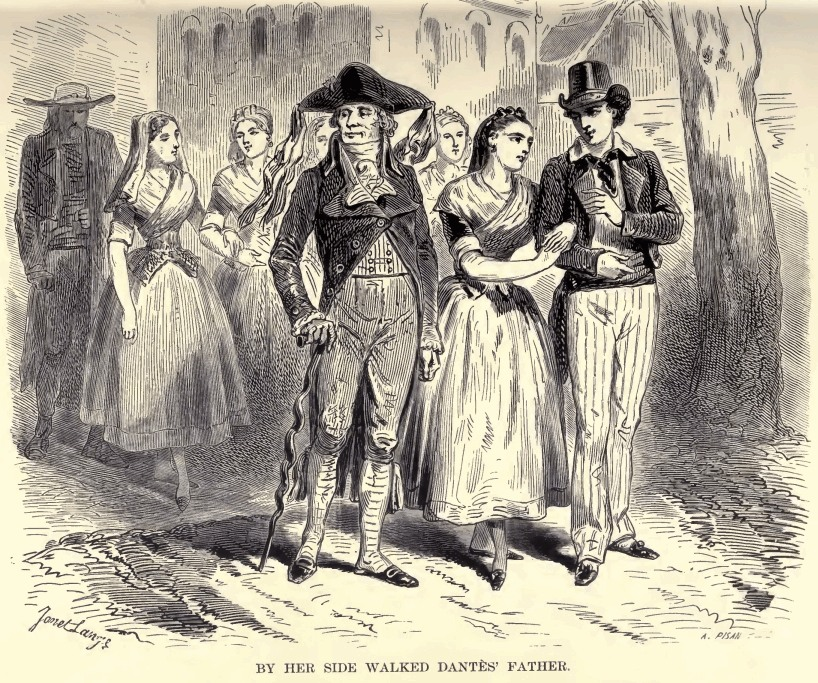
\includegraphics[width=\textwidth]{0065m.jpg}
\end{figure}

As Danglars approached the disappointed lover, he cast on him a look of
deep meaning, while Fernand, as he slowly paced behind the happy pair,
who seemed, in their own unmixed content, to have entirely forgotten
that such a being as himself existed, was pale and abstracted;
occasionally, however, a deep flush would overspread his countenance,
and a nervous contraction distort his features, while, with an agitated
and restless gaze, he would glance in the direction of Marseilles, like
one who either anticipated or foresaw some great and important event.

Dantès himself was simply, but becomingly, clad in the dress peculiar
to the merchant service—a costume somewhat between a military and a
civil garb; and with his fine countenance, radiant with joy and
happiness, a more perfect specimen of manly beauty could scarcely be
imagined.

Lovely as the Greek girls of Cyprus or Chios, Mercédès boasted the same
bright flashing eyes of jet, and ripe, round, coral lips. She moved
with the light, free step of an Arlesienne or an Andalusian. One more
practiced in the arts of great cities would have hid her blushes
beneath a veil, or, at least, have cast down her thickly fringed
lashes, so as to have concealed the liquid lustre of her animated eyes;
but, on the contrary, the delighted girl looked around her with a smile
that seemed to say: “If you are my friends, rejoice with me, for I am
very happy.”

As soon as the bridal party came in sight of La Réserve, M. Morrel
descended and came forth to meet it, followed by the soldiers and
sailors there assembled, to whom he had repeated the promise already
given, that Dantès should be the successor to the late Captain Leclere.
Edmond, at the approach of his patron, respectfully placed the arm of
his affianced bride within that of M. Morrel, who, forthwith conducting
her up the flight of wooden steps leading to the chamber in which the
feast was prepared, was gayly followed by the guests, beneath whose
heavy tread the slight structure creaked and groaned for the space of
several minutes.

“Father,” said Mercédès, stopping when she had reached the centre of
the table, “sit, I pray you, on my right hand; on my left I will place
him who has ever been as a brother to me,” pointing with a soft and
gentle smile to Fernand; but her words and look seemed to inflict the
direst torture on him, for his lips became ghastly pale, and even
beneath the dark hue of his complexion the blood might be seen
retreating as though some sudden pang drove it back to the heart.

During this time, Dantès, at the opposite side of the table, had been
occupied in similarly placing his most honored guests. M. Morrel was
seated at his right hand, Danglars at his left; while, at a sign from
Edmond, the rest of the company ranged themselves as they found it most
agreeable.

Then they began to pass around the dusky, piquant, Arlesian sausages,
and lobsters in their dazzling red cuirasses, prawns of large size and
brilliant color, the echinus with its prickly outside and dainty morsel
within, the clovis, esteemed by the epicures of the South as more than
rivalling the exquisite flavor of the oyster, North. All the
delicacies, in fact, that are cast up by the wash of waters on the
sandy beach, and styled by the grateful fishermen “fruits of the sea.”

“A pretty silence truly!” said the old father of the bridegroom, as he
carried to his lips a glass of wine of the hue and brightness of the
topaz, and which had just been placed before Mercédès herself. “Now,
would anybody think that this room contained a happy, merry party, who
desire nothing better than to laugh and dance the hours away?”

“Ah,” sighed Caderousse, “a man cannot always feel happy because he is
about to be married.”

“The truth is,” replied Dantès, “that I am too happy for noisy mirth;
if that is what you meant by your observation, my worthy friend, you
are right; joy takes a strange effect at times, it seems to oppress us
almost the same as sorrow.”

Danglars looked towards Fernand, whose excitable nature received and
betrayed each fresh impression.

“Why, what ails you?” asked he of Edmond. “Do you fear any approaching
evil? I should say that you were the happiest man alive at this
instant.”

“And that is the very thing that alarms me,” returned Dantès. “Man does
not appear to me to be intended to enjoy felicity so unmixed; happiness
is like the enchanted palaces we read of in our childhood, where
fierce, fiery dragons defend the entrance and approach; and monsters of
all shapes and kinds, requiring to be overcome ere victory is ours. I
own that I am lost in wonder to find myself promoted to an honor of
which I feel myself unworthy—that of being the husband of Mercédès.”

“Nay, nay!” cried Caderousse, smiling, “you have not attained that
honor yet. Mercédès is not yet your wife. Just assume the tone and
manner of a husband, and see how she will remind you that your hour is
not yet come!”

The bride blushed, while Fernand, restless and uneasy, seemed to start
at every fresh sound, and from time to time wiped away the large drops
of perspiration that gathered on his brow.

“Well, never mind that, neighbor Caderousse; it is not worthwhile to
contradict me for such a trifle as that. ’Tis true that Mercédès is not
actually my wife; but,” added he, drawing out his watch, “in an hour
and a half she will be.”

A general exclamation of surprise ran round the table, with the
exception of the elder Dantès, whose laugh displayed the still perfect
beauty of his large white teeth. Mercédès looked pleased and gratified,
while Fernand grasped the handle of his knife with a convulsive clutch.

“In an hour?” inquired Danglars, turning pale. “How is that, my
friend?”

“Why, thus it is,” replied Dantès. “Thanks to the influence of M.
Morrel, to whom, next to my father, I owe every blessing I enjoy, every
difficulty has been removed. We have purchased permission to waive the
usual delay; and at half-past two o’clock the Mayor of Marseilles will
be waiting for us at the city hall. Now, as a quarter-past one has
already struck, I do not consider I have asserted too much in saying,
that, in another hour and thirty minutes Mercédès will have become
Madame Dantès.”

\begin{figure}[ht]
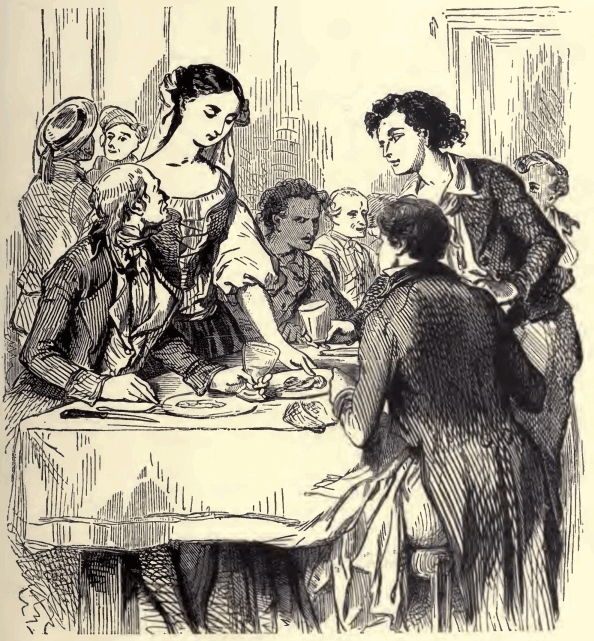
\includegraphics[width=\textwidth]{0069m.jpg}
\end{figure}

Fernand closed his eyes, a burning sensation passed across his brow,
and he was compelled to support himself by the table to prevent his
falling from his chair; but in spite of all his efforts, he could not
refrain from uttering a deep groan, which, however, was lost amid the
noisy felicitations of the company.

“Upon my word,” cried the old man, “you make short work of this kind of
affair. Arrived here only yesterday morning, and married today at three
o’clock! Commend me to a sailor for going the quick way to work!”

“But,” asked Danglars, in a timid tone, “how did you manage about the
other formalities—the contract—the settlement?”

“The contract,” answered Dantès, laughingly, “it didn’t take long to
fix that. Mercédès has no fortune; I have none to settle on her. So,
you see, our papers were quickly written out, and certainly do not come
very expensive.” This joke elicited a fresh burst of applause.

“So that what we presumed to be merely the betrothal feast turns out to
be the actual wedding dinner!” said Danglars.

“No, no,” answered Dantès; “don’t imagine I am going to put you off in
that shabby manner. Tomorrow morning I start for Paris; four days to
go, and the same to return, with one day to discharge the commission
entrusted to me, is all the time I shall be absent. I shall be back
here by the first of March, and on the second I give my real marriage
feast.”

This prospect of fresh festivity redoubled the hilarity of the guests
to such a degree, that the elder Dantès, who, at the commencement of
the repast, had commented upon the silence that prevailed, now found it
difficult, amid the general din of voices, to obtain a moment’s
tranquillity in which to drink to the health and prosperity of the
bride and bridegroom.

Dantès, perceiving the affectionate eagerness of his father, responded
by a look of grateful pleasure; while Mercédès glanced at the clock and
made an expressive gesture to Edmond.

Around the table reigned that noisy hilarity which usually prevails at
such a time among people sufficiently free from the demands of social
position not to feel the trammels of etiquette. Such as at the
commencement of the repast had not been able to seat themselves
according to their inclination rose unceremoniously, and sought out
more agreeable companions. Everybody talked at once, without waiting
for a reply and each one seemed to be contented with expressing his or
her own thoughts.

Fernand’s paleness appeared to have communicated itself to Danglars. As
for Fernand himself, he seemed to be enduring the tortures of the
damned; unable to rest, he was among the first to quit the table, and,
as though seeking to avoid the hilarious mirth that rose in such
deafening sounds, he continued, in utter silence, to pace the farther
end of the salon.

Caderousse approached him just as Danglars, whom Fernand seemed most
anxious to avoid, had joined him in a corner of the room.

“Upon my word,” said Caderousse, from whose mind the friendly treatment
of Dantès, united with the effect of the excellent wine he had partaken
of, had effaced every feeling of envy or jealousy at Dantès’ good
fortune,—“upon my word, Dantès is a downright good fellow, and when I
see him sitting there beside his pretty wife that is so soon to be. I
cannot help thinking it would have been a great pity to have served him
that trick you were planning yesterday.”

“Oh, there was no harm meant,” answered Danglars; “at first I certainly
did feel somewhat uneasy as to what Fernand might be tempted to do; but
when I saw how completely he had mastered his feelings, even so far as
to become one of his rival’s attendants, I knew there was no further
cause for apprehension.” Caderousse looked full at Fernand—he was
ghastly pale.

“Certainly,” continued Danglars, “the sacrifice was no trifling one,
when the beauty of the bride is concerned. Upon my soul, that future
captain of mine is a lucky dog! Gad! I only wish he would let me take
his place.”

“Shall we not set forth?” asked the sweet, silvery voice of Mercédès;
“two o’clock has just struck, and you know we are expected in a quarter
of an hour.”

\begin{figure}[ht]
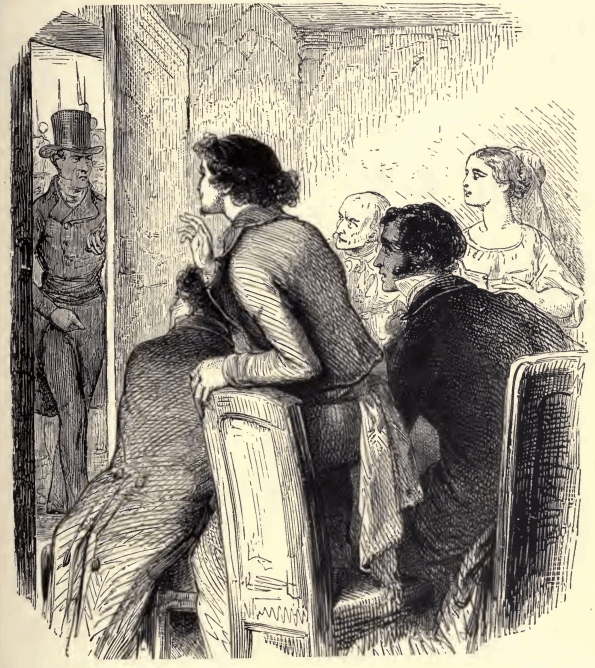
\includegraphics[width=\textwidth]{0071m.jpg}
\end{figure}

“To be sure!—to be sure!” cried Dantès, eagerly quitting the table;
“let us go directly!”

His words were re-echoed by the whole party, with vociferous cheers.

At this moment Danglars, who had been incessantly observing every
change in Fernand’s look and manner, saw him stagger and fall back,
with an almost convulsive spasm, against a seat placed near one of the
open windows. At the same instant his ear caught a sort of indistinct
sound on the stairs, followed by the measured tread of soldiery, with
the clanking of swords and military accoutrements; then came a hum and
buzz as of many voices, so as to deaden even the noisy mirth of the
bridal party, among whom a vague feeling of curiosity and apprehension
quelled every disposition to talk, and almost instantaneously the most
deathlike stillness prevailed.

The sounds drew nearer. Three blows were struck upon the panel of the
door. The company looked at each other in consternation.

“I demand admittance,” said a loud voice outside the room, “in the name
of the law!” As no attempt was made to prevent it, the door was opened,
and a magistrate, wearing his official scarf, presented himself,
followed by four soldiers and a corporal. Uneasiness now yielded to the
most extreme dread on the part of those present.

“May I venture to inquire the reason of this unexpected visit?” said M.
Morrel, addressing the magistrate, whom he evidently knew; “there is
doubtless some mistake easily explained.”

“If it be so,” replied the magistrate, “rely upon every reparation
being made; meanwhile, I am the bearer of an order of arrest, and
although I most reluctantly perform the task assigned me, it must,
nevertheless, be fulfilled. Who among the persons here assembled
answers to the name of Edmond Dantès?”

Every eye was turned towards the young man who, spite of the agitation
he could not but feel, advanced with dignity, and said, in a firm
voice:

“I am he; what is your pleasure with me?”

“Edmond Dantès,” replied the magistrate, “I arrest you in the name of
the law!”

“Me!” repeated Edmond, slightly changing color, “and wherefore, I
pray?”

“I cannot inform you, but you will be duly acquainted with the reasons
that have rendered such a step necessary at the preliminary
examination.”

M. Morrel felt that further resistance or remonstrance was useless. He
saw before him an officer delegated to enforce the law, and perfectly
well knew that it would be as unavailing to seek pity from a magistrate
decked with his official scarf, as to address a petition to some cold
marble effigy. Old Dantès, however, sprang forward. There are
situations which the heart of a father or a mother cannot be made to
understand. He prayed and supplicated in terms so moving, that even the
officer was touched, and, although firm in his duty, he kindly said,
“My worthy friend, let me beg of you to calm your apprehensions. Your
son has probably neglected some prescribed form or attention in
registering his cargo, and it is more than probable he will be set at
liberty directly he has given the information required, whether
touching the health of his crew, or the value of his freight.”

“What is the meaning of all this?” inquired Caderousse, frowningly, of
Danglars, who had assumed an air of utter surprise.

\begin{figure}[h]
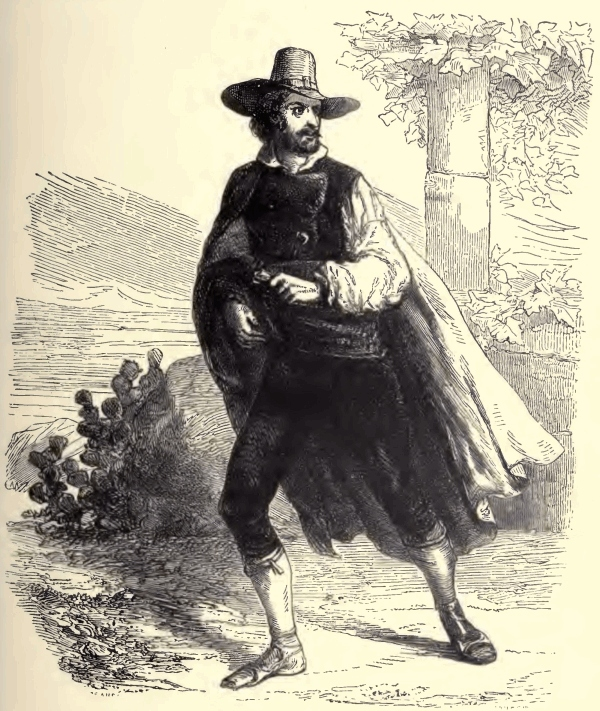
\includegraphics[width=\textwidth]{0073m.jpg}
\end{figure}

“How can I tell you?” replied he; “I am, like yourself, utterly
bewildered at all that is going on, and cannot in the least make out
what it is about.” Caderousse then looked around for Fernand, but he
had disappeared.

The scene of the previous night now came back to his mind with
startling clearness. The painful catastrophe he had just witnessed
appeared effectually to have rent away the veil which the intoxication
of the evening before had raised between himself and his memory.

“So, so,” said he, in a hoarse and choking voice, to Danglars, “this,
then, I suppose, is a part of the trick you were concerting yesterday?
All I can say is, that if it be so, ’tis an ill turn, and well deserves
to bring double evil on those who have projected it.”

“Nonsense,” returned Danglars, “I tell you again I have nothing
whatever to do with it; besides, you know very well that I tore the
paper to pieces.”

“No, you did not!” answered Caderousse, “you merely threw it by—I saw
it lying in a corner.”

“Hold your tongue, you fool!—what should you know about it?—why, you
were drunk!”

“Where is Fernand?” inquired Caderousse.

“How do I know?” replied Danglars; “gone, as every prudent man ought to
be, to look after his own affairs, most likely. Never mind where he is,
let you and I go and see what is to be done for our poor friends.”

During this conversation, Dantès, after having exchanged a cheerful
shake of the hand with all his sympathizing friends, had surrendered
himself to the officer sent to arrest him, merely saying, “Make
yourselves quite easy, my good fellows, there is some little mistake to
clear up, that’s all, depend upon it; and very likely I may not have to
go so far as the prison to effect that.”

\begin{figure}[ht]
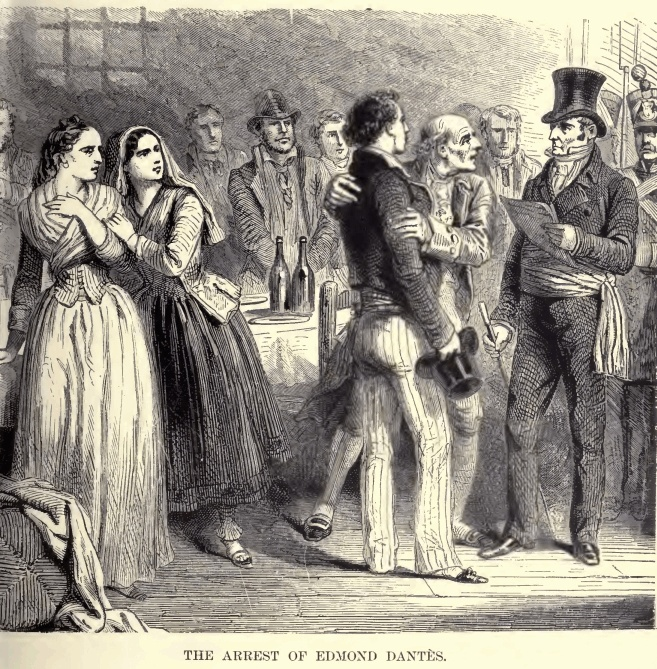
\includegraphics[width=\textwidth]{0075m.jpg}
\end{figure}

“Oh, to be sure!” responded Danglars, who had now approached the group,
“nothing more than a mistake, I feel quite certain.”

Dantès descended the staircase, preceded by the magistrate, and
followed by the soldiers. A carriage awaited him at the door; he got
in, followed by two soldiers and the magistrate, and the vehicle drove
off towards Marseilles.

“Adieu, adieu, dearest Edmond!” cried Mercédès, stretching out her arms
to him from the balcony.

The prisoner heard the cry, which sounded like the sob of a broken
heart, and leaning from the coach he called out, “Good-bye, Mercédès—we
shall soon meet again!” Then the vehicle disappeared round one of the
turnings of Fort Saint Nicholas.

“Wait for me here, all of you!” cried M. Morrel; “I will take the first
conveyance I find, and hurry to Marseilles, whence I will bring you
word how all is going on.”

“That’s right!” exclaimed a multitude of voices, “go, and return as
quickly as you can!”

This second departure was followed by a long and fearful state of
terrified silence on the part of those who were left behind. The old
father and Mercédès remained for some time apart, each absorbed in
grief; but at length the two poor victims of the same blow raised their
eyes, and with a simultaneous burst of feeling rushed into each other’s
arms.

Meanwhile Fernand made his appearance, poured out for himself a glass
of water with a trembling hand; then hastily swallowing it, went to sit
down at the first vacant place, and this was, by mere chance, placed
next to the seat on which poor Mercédès had fallen half fainting, when
released from the warm and affectionate embrace of old Dantès.
Instinctively Fernand drew back his chair.

“He is the cause of all this misery—I am quite sure of it,” whispered
Caderousse, who had never taken his eyes off Fernand, to Danglars.

“I don’t think so,” answered the other; “he’s too stupid to imagine
such a scheme. I only hope the mischief will fall upon the head of
whoever wrought it.”

“You don’t mention those who aided and abetted the deed,” said
Caderousse.

“Surely,” answered Danglars, “one cannot be held responsible for every
chance arrow shot into the air.”

“You can, indeed, when the arrow lights point downward on somebody’s
head.”

Meantime the subject of the arrest was being canvassed in every
different form.

“What think you, Danglars,” said one of the party, turning towards him,
“of this event?”

“Why,” replied he, “I think it just possible Dantès may have been
detected with some trifling article on board ship considered here as
contraband.”

“But how could he have done so without your knowledge, Danglars, since
you are the ship’s supercargo?”

“Why, as for that, I could only know what I was told respecting the
merchandise with which the vessel was laden. I know she was loaded with
cotton, and that she took in her freight at Alexandria from Pastret’s
warehouse, and at Smyrna from Pascal’s; that is all I was obliged to
know, and I beg I may not be asked for any further particulars.”

“Now I recollect,” said the afflicted old father; “my poor boy told me
yesterday he had got a small case of coffee, and another of tobacco for
me!”

“There, you see,” exclaimed Danglars. “Now the mischief is out; depend
upon it the custom-house people went rummaging about the ship in our
absence, and discovered poor Dantès’ hidden treasures.”

Mercédès, however, paid no heed to this explanation of her lover’s
arrest. Her grief, which she had hitherto tried to restrain, now burst
out in a violent fit of hysterical sobbing.

“Come, come,” said the old man, “be comforted, my poor child; there is
still hope!”

“Hope!” repeated Danglars.

“Hope!” faintly murmured Fernand, but the word seemed to die away on
his pale agitated lips, and a convulsive spasm passed over his
countenance.

“Good news! good news!” shouted forth one of the party stationed in the
balcony on the lookout. “Here comes M. Morrel back. No doubt, now, we
shall hear that our friend is released!”

Mercédès and the old man rushed to meet the shipowner and greeted him
at the door. He was very pale.

“What news?” exclaimed a general burst of voices.

“Alas, my friends,” replied M. Morrel, with a mournful shake of his
head, “the thing has assumed a more serious aspect than I expected.”

“Oh, indeed—indeed, sir, he is innocent!” sobbed forth Mercédès.

“That I believe!” answered M. Morrel; “but still he is charged——”

“With what?” inquired the elder Dantès.

“With being an agent of the Bonapartist faction!” Many of our readers
may be able to recollect how formidable such an accusation became in
the period at which our story is dated.

A despairing cry escaped the pale lips of Mercédès; the old man sank
into a chair.

“Ah, Danglars!” whispered Caderousse, “you have deceived me—the trick
you spoke of last night has been played; but I cannot suffer a poor old
man or an innocent girl to die of grief through your fault. I am
determined to tell them all about it.”

“Be silent, you simpleton!” cried Danglars, grasping him by the arm,
“or I will not answer even for your own safety. Who can tell whether
Dantès be innocent or guilty? The vessel did touch at Elba, where he
quitted it, and passed a whole day in the island. Now, should any
letters or other documents of a compromising character be found upon
him, will it not be taken for granted that all who uphold him are his
accomplices?”

With the rapid instinct of selfishness, Caderousse readily perceived
the solidity of this mode of reasoning; he gazed, doubtfully,
wistfully, on Danglars, and then caution supplanted generosity.

“Suppose we wait a while, and see what comes of it,” said he, casting a
bewildered look on his companion.

“To be sure!” answered Danglars. “Let us wait, by all means. If he be
innocent, of course he will be set at liberty; if guilty, why, it is no
use involving ourselves in a conspiracy.”

“Let us go, then. I cannot stay here any longer.”

“With all my heart!” replied Danglars, pleased to find the other so
tractable. “Let us take ourselves out of the way, and leave things for
the present to take their course.”

After their departure, Fernand, who had now again become the friend and
protector of Mercédès, led the girl to her home, while some friends of
Dantès conducted his father, nearly lifeless, to the Allées de Meilhan.

The rumor of Edmond’s arrest as a Bonapartist agent was not slow in
circulating throughout the city.

“Could you ever have credited such a thing, my dear Danglars?” asked M.
Morrel, as, on his return to the port for the purpose of gleaning fresh
tidings of Dantès, from M. de Villefort, the assistant procureur, he
overtook his supercargo and Caderousse. “Could you have believed such a
thing possible?”

“Why, you know I told you,” replied Danglars, “that I considered the
circumstance of his having anchored at the Island of Elba as a very
suspicious circumstance.”

“And did you mention these suspicions to any person beside myself?”

\begin{figure}[ht]
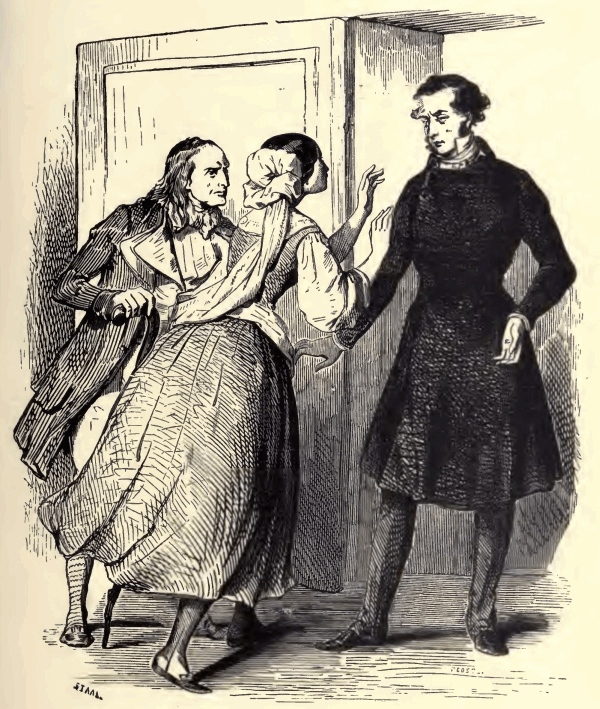
\includegraphics[width=\textwidth]{0079m.jpg}
\end{figure}

“Certainly not!” returned Danglars. Then added in a low whisper, “You
understand that, on account of your uncle, M. Policar Morrel, who
served under the \textit{other} government, and who does not altogether
conceal what he thinks on the subject, you are strongly suspected of
regretting the abdication of Napoleon. I should have feared to injure
both Edmond and yourself, had I divulged my own apprehensions to a
soul. I am too well aware that though a subordinate, like myself, is
bound to acquaint the shipowner with everything that occurs, there are
many things he ought most carefully to conceal from all else.”

“’Tis well, Danglars—’tis well!” replied M. Morrel. “You are a worthy
fellow; and I had already thought of your interests in the event of
poor Edmond having become captain of the \textit{Pharaon}.”

“Is it possible you were so kind?”

“Yes, indeed; I had previously inquired of Dantès what was his opinion
of you, and if he should have any reluctance to continue you in your
post, for somehow I have perceived a sort of coolness between you.”

“And what was his reply?”

“That he certainly did think he had given you offence in an affair
which he merely referred to without entering into particulars, but that
whoever possessed the good opinion and confidence of the ship’s owners
would have his preference also.”

“The hypocrite!” murmured Danglars.

“Poor Dantès!” said Caderousse. “No one can deny his being a
noble-hearted young fellow.”

“But meanwhile,” continued M. Morrel, “here is the \textit{Pharaon} without a
captain.”

“Oh,” replied Danglars, “since we cannot leave this port for the next
three months, let us hope that ere the expiration of that period Dantès
will be set at liberty.”

“No doubt; but in the meantime?”

“I am entirely at your service, M. Morrel,” answered Danglars. “You
know that I am as capable of managing a ship as the most experienced
captain in the service; and it will be so far advantageous to you to
accept my services, that upon Edmond’s release from prison no further
change will be requisite on board the \textit{Pharaon} than for Dantès and
myself each to resume our respective posts.”

“Thanks, Danglars—that will smooth over all difficulties. I fully
authorize you at once to assume the command of the \textit{Pharaon}, and look
carefully to the unloading of her freight. Private misfortunes must
never be allowed to interfere with business.”

“Be easy on that score, M. Morrel; but do you think we shall be
permitted to see our poor Edmond?”

“I will let you know that directly I have seen M. de Villefort, whom I
shall endeavor to interest in Edmond’s favor. I am aware he is a
furious royalist; but, in spite of that, and of his being king’s
attorney, he is a man like ourselves, and I fancy not a bad sort of
one.”

“Perhaps not,” replied Danglars; “but I hear that he is ambitious, and
that’s rather against him.”

“Well, well,” returned M. Morrel, “we shall see. But now hasten on
board, I will join you there ere long.”

So saying, the worthy shipowner quitted the two allies, and proceeded
in the direction of the Palais de Justice.

\begin{figure}[h]
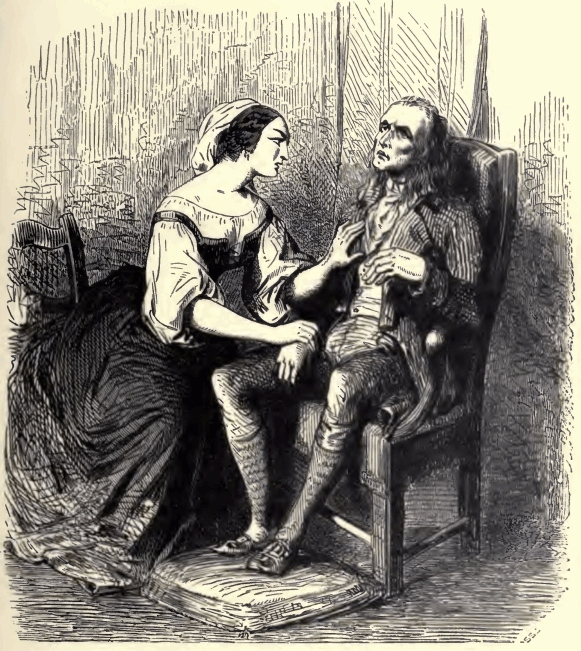
\includegraphics[width=\textwidth]{0081m.jpg}
\end{figure}

“You see,” said Danglars, addressing Caderousse, “the turn things have
taken. Do you still feel any desire to stand up in his defence?”

“Not the slightest, but yet it seems to me a shocking thing that a mere
joke should lead to such consequences.”

“But who perpetrated that joke, let me ask? neither you nor myself, but
Fernand; you knew very well that I threw the paper into a corner of the
room—indeed, I fancied I had destroyed it.”

“Oh, no,” replied Caderousse, “that I can answer for, you did not. I
only wish I could see it now as plainly as I saw it lying all crushed
and crumpled in a corner of the arbor.”

“Well, then, if you did, depend upon it, Fernand picked it up, and
either copied it or caused it to be copied; perhaps, even, he did not
take the trouble of recopying it. And now I think of it, by Heavens, he
may have sent the letter itself! Fortunately, for me, the handwriting
was disguised.”

“Then you were aware of Dantès being engaged in a conspiracy?”

“Not I. As I before said, I thought the whole thing was a joke, nothing
more. It seems, however, that I have unconsciously stumbled upon the
truth.”

“Still,” argued Caderousse, “I would give a great deal if nothing of
the kind had happened; or, at least, that I had had no hand in it. You
will see, Danglars, that it will turn out an unlucky job for both of
us.”

“Nonsense! If any harm come of it, it should fall on the guilty person;
and that, you know, is Fernand. How can we be implicated in any way?
All we have got to do is, to keep our own counsel, and remain perfectly
quiet, not breathing a word to any living soul; and you will see that
the storm will pass away without in the least affecting us.”

“Amen!” responded Caderousse, waving his hand in token of adieu to
Danglars, and bending his steps towards the Allées de Meilhan, moving
his head to and fro, and muttering as he went, after the manner of one
whose mind was overcharged with one absorbing idea.

“So far, then,” said Danglars, mentally, “all has gone as I would have
it. I am, temporarily, commander of the \textit{Pharaon}, with the certainty
of being permanently so, if that fool of a Caderousse can be persuaded
to hold his tongue. My only fear is the chance of Dantès being
released. But, there, he is in the hands of Justice; and,” added he
with a smile, “she will take her own.” So saying, he leaped into a
boat, desiring to be rowed on board the \textit{Pharaon}, where M. Morrel had
agreed to meet him.

\printpagenotes*
\chapter{The Deputy Procureur du Roi}

In one of the aristocratic mansions built by Puget in the Rue du Grand
Cours opposite the Medusa fountain, a second marriage feast was being
celebrated, almost at the same hour with the nuptial repast given by
Dantès. In this case, however, although the occasion of the
entertainment was similar, the company was strikingly dissimilar.
Instead of a rude mixture of sailors, soldiers, and those belonging to
the humblest grade of life, the present assembly was composed of the
very flower of Marseilles society,—magistrates who had resigned their
office during the usurper’s reign; officers who had deserted from the
imperial army and joined forces with Condé; and younger members of
families, brought up to hate and execrate the man whom five years of
exile would convert into a martyr, and fifteen of restoration elevate
to the rank of a god.

The guests were still at table, and the heated and energetic
conversation that prevailed betrayed the violent and vindictive
passions that then agitated each dweller of the South, where unhappily,
for five centuries religious strife had long given increased bitterness
to the violence of party feeling.

The emperor, now king of the petty Island of Elba, after having held
sovereign sway over one-half of the world, counting as his subjects a
small population of five or six thousand souls,—after having been
accustomed to hear the “\textit{Vive Napoléons}” of a hundred and twenty
millions of human beings, uttered in ten different languages,—was
looked upon here as a ruined man, separated forever from any fresh
connection with France or claim to her throne.

The magistrates freely discussed their political views; the military
part of the company talked unreservedly of Moscow and Leipsic, while
the women commented on the divorce of Josephine. It was not over the
downfall of the man, but over the defeat of the Napoleonic idea, that
they rejoiced, and in this they foresaw for themselves the bright and
cheering prospect of a revivified political existence.

An old man, decorated with the cross of Saint Louis, now rose and
proposed the health of King Louis XVIII. It was the Marquis de
Saint-Méran. This toast, recalling at once the patient exile of
Hartwell and the peace-loving King of France, excited universal
enthusiasm; glasses were elevated in the air \textit{à l’Anglaise}, and the
ladies, snatching their bouquets from their fair bosoms, strewed the
table with their floral treasures. In a word, an almost poetical fervor
prevailed.

“Ah,” said the Marquise de Saint-Méran, a woman with a stern,
forbidding eye, though still noble and distinguished in appearance,
despite her fifty years—“ah, these revolutionists, who have driven us
from those very possessions they afterwards purchased for a mere trifle
during the Reign of Terror, would be compelled to own, were they here,
that all true devotion was on our side, since we were content to follow
the fortunes of a falling monarch, while they, on the contrary, made
their fortune by worshipping the rising sun; yes, yes, they could not
help admitting that the king, for whom we sacrificed rank, wealth, and
station was truly our ‘Louis the well-beloved,’ while their wretched
usurper has been, and ever will be, to them their evil genius, their
‘Napoleon the accursed.’ Am I not right, Villefort?”

“I beg your pardon, madame. I really must pray you to excuse me, but—in
truth—I was not attending to the conversation.”

“Marquise, marquise!” interposed the old nobleman who had proposed the
toast, “let the young people alone; let me tell you, on one’s wedding
day there are more agreeable subjects of conversation than dry
politics.”

“Never mind, dearest mother,” said a young and lovely girl, with a
profusion of light brown hair, and eyes that seemed to float in liquid
crystal, “’tis all my fault for seizing upon M. de Villefort, so as to
prevent his listening to what you said. But there—now take him—he is
your own for as long as you like. M. Villefort, I beg to remind you my
mother speaks to you.”

“If the marquise will deign to repeat the words I but imperfectly
caught, I shall be delighted to answer,” said M. de Villefort.

“Never mind, Renée,” replied the marquise, with a look of tenderness
that seemed out of keeping with her harsh dry features; but, however
all other feelings may be withered in a woman’s nature, there is always
one bright smiling spot in the desert of her heart, and that is the
shrine of maternal love. “I forgive you. What I was saying, Villefort,
was, that the Bonapartists had not our sincerity, enthusiasm, or
devotion.”

“They had, however, what supplied the place of those fine qualities,”
replied the young man, “and that was fanaticism. Napoleon is the
Mahomet of the West, and is worshipped by his commonplace but ambitious
followers, not only as a leader and lawgiver, but also as the
personification of equality.”

“He!” cried the marquise: “Napoleon the type of equality! For mercy’s
sake, then, what would you call Robespierre? Come, come, do not strip
the latter of his just rights to bestow them on the Corsican, who, to
my mind, has usurped quite enough.”

\begin{figure}[h]
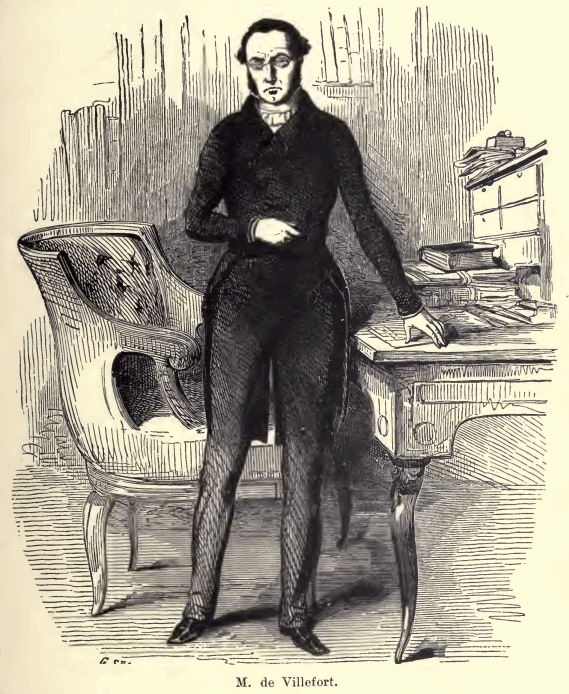
\includegraphics[width=\textwidth]{0085m.jpg}
\end{figure}

“Nay, madame; I would place each of these heroes on his right
pedestal—that of Robespierre on his scaffold in the Place Louis Quinze;
that of Napoleon on the column of the Place Vendôme. The only
difference consists in the opposite character of the equality advocated
by these two men; one is the equality that elevates, the other is the
equality that degrades; one brings a king within reach of the
guillotine, the other elevates the people to a level with the throne.
Observe,” said Villefort, smiling, “I do not mean to deny that both
these men were revolutionary scoundrels, and that the 9th Thermidor and
the 4th of April, in the year 1814, were lucky days for France, worthy
of being gratefully remembered by every friend to monarchy and civil
order; and that explains how it comes to pass that, fallen, as I trust
he is forever, Napoleon has still retained a train of parasitical
satellites. Still, marquise, it has been so with other
usurpers—Cromwell, for instance, who was not half so bad as Napoleon,
had his partisans and advocates.”

“Do you know, Villefort, that you are talking in a most dreadfully
revolutionary strain? But I excuse it, it is impossible to expect the
son of a Girondin to be free from a small spice of the old leaven.” A
deep crimson suffused the countenance of Villefort.

“’Tis true, madame,” answered he, “that my father was a Girondin, but
he was not among the number of those who voted for the king’s death; he
was an equal sufferer with yourself during the Reign of Terror, and had
well-nigh lost his head on the same scaffold on which your father
perished.”

“True,” replied the marquise, without wincing in the slightest degree
at the tragic remembrance thus called up; “but bear in mind, if you
please, that our respective parents underwent persecution and
proscription from diametrically opposite principles; in proof of which
I may remark, that while my family remained among the staunchest
adherents of the exiled princes, your father lost no time in joining
the new government; and that while the Citizen Noirtier was a Girondin,
the Count Noirtier became a senator.”

“Dear mother,” interposed Renée, “you know very well it was agreed that
all these disagreeable reminiscences should forever be laid aside.”

“Suffer me, also, madame,” replied Villefort, “to add my earnest
request to Mademoiselle de Saint-Méran’s, that you will kindly allow
the veil of oblivion to cover and conceal the past. What avails
recrimination over matters wholly past recall? For my own part, I have
laid aside even the name of my father, and altogether disown his
political principles. He was—nay, probably may still be—a Bonapartist,
and is called Noirtier; I, on the contrary, am a staunch royalist, and
style myself de Villefort. Let what may remain of revolutionary sap
exhaust itself and die away with the old trunk, and condescend only to
regard the young shoot which has started up at a distance from the
parent tree, without having the power, any more than the wish, to
separate entirely from the stock from which it sprung.”

“Bravo, Villefort!” cried the marquis; “excellently well said! Come,
now, I have hopes of obtaining what I have been for years endeavoring
to persuade the marquise to promise; namely, a perfect amnesty and
forgetfulness of the past.”

“With all my heart,” replied the marquise; “let the past be forever
forgotten. I promise you it affords \textit{me} as little pleasure to revive
it as it does you. All I ask is, that Villefort will be firm and
inflexible for the future in his political principles. Remember, also,
Villefort, that we have pledged ourselves to his majesty for your
fealty and strict loyalty, and that at our recommendation the king
consented to forget the past, as I do” (and here she extended to him
her hand)—“as I now do at your entreaty. But bear in mind, that should
there fall in your way anyone guilty of conspiring against the
government, you will be so much the more bound to visit the offence
with rigorous punishment, as it is known you belong to a suspected
family.”

“Alas, madame,” returned Villefort, “my profession, as well as the
times in which we live, compels me to be severe. I have already
successfully conducted several public prosecutions, and brought the
offenders to merited punishment. But we have not done with the thing
yet.”

\begin{figure}[h]
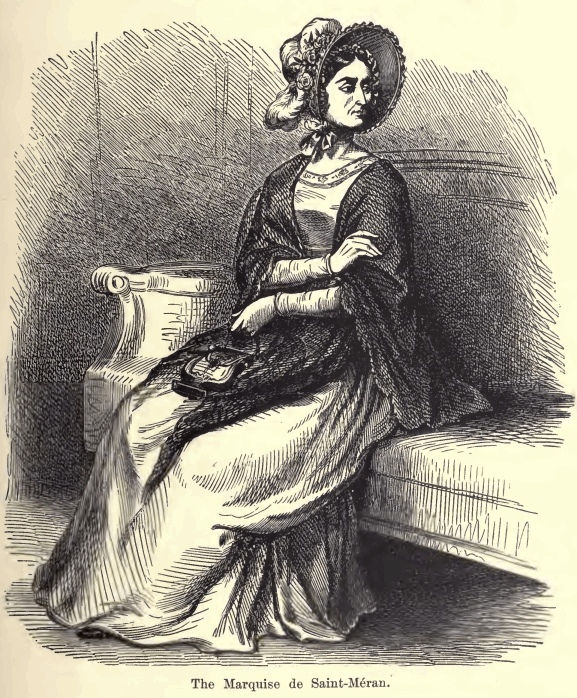
\includegraphics[width=\textwidth]{0087m.jpg}
\end{figure}

“Do you, indeed, think so?” inquired the marquise.

“I am, at least, fearful of it. Napoleon, in the Island of Elba, is too
near France, and his proximity keeps up the hopes of his partisans.
Marseilles is filled with half-pay officers, who are daily, under one
frivolous pretext or other, getting up quarrels with the royalists;
from hence arise continual and fatal duels among the higher classes of
persons, and assassinations in the lower.”

“You have heard, perhaps,” said the Comte de Salvieux, one of M. de
Saint-Méran’s oldest friends, and chamberlain to the Comte d’Artois,
“that the Holy Alliance purpose removing him from thence?”

“Yes; they were talking about it when we left Paris,” said M. de
Saint-Méran; “and where is it decided to transfer him?”

“To Saint Helena.”

“For heaven’s sake, where is that?” asked the marquise.

“An island situated on the other side of the equator, at least two
thousand leagues from here,” replied the count.

“So much the better. As Villefort observes, it is a great act of folly
to have left such a man between Corsica, where he was born, and Naples,
of which his brother-in-law is king, and face to face with Italy, the
sovereignty of which he coveted for his son.”

“Unfortunately,” said Villefort, “there are the treaties of 1814, and
we cannot molest Napoleon without breaking those compacts.”

“Oh, well, we shall find some way out of it,” responded M. de Salvieux.
“There wasn’t any trouble over treaties when it was a question of
shooting the poor Duc d’Enghien.”

“Well,” said the marquise, “it seems probable that, by the aid of the
Holy Alliance, we shall be rid of Napoleon; and we must trust to the
vigilance of M. de Villefort to purify Marseilles of his partisans. The
king is either a king or no king; if he be acknowledged as sovereign of
France, he should be upheld in peace and tranquillity; and this can
best be effected by employing the most inflexible agents to put down
every attempt at conspiracy—’tis the best and surest means of
preventing mischief.”

“Unfortunately, madame,” answered Villefort, “the strong arm of the law
is not called upon to interfere until the evil has taken place.”

“Then all he has got to do is to endeavor to repair it.”

“Nay, madame, the law is frequently powerless to effect this; all it
can do is to avenge the wrong done.”

“Oh, M. de Villefort,” cried a beautiful young creature, daughter to
the Comte de Salvieux, and the cherished friend of Mademoiselle de
Saint-Méran, “do try and get up some famous trial while we are at
Marseilles. I never was in a law-court; I am told it is so very
amusing!”

“Amusing, certainly,” replied the young man, “inasmuch as, instead of
shedding tears as at the fictitious tale of woe produced at a theatre,
you behold in a law-court a case of real and genuine distress—a drama
of life. The prisoner whom you there see pale, agitated, and alarmed,
instead of—as is the case when a curtain falls on a tragedy—going home
to sup peacefully with his family, and then retiring to rest, that he
may recommence his mimic woes on the morrow,—is removed from your sight
merely to be reconducted to his prison and delivered up to the
executioner. I leave you to judge how far your nerves are calculated to
bear you through such a scene. Of this, however, be assured, that
should any favorable opportunity present itself, I will not fail to
offer you the choice of being present.”

“For shame, M. de Villefort!” said Renée, becoming quite pale; “don’t
you see how you are frightening us?—and yet you laugh.”

“What would you have? ’Tis like a duel. I have already recorded
sentence of death, five or six times, against the movers of political
conspiracies, and who can say how many daggers may be ready sharpened,
and only waiting a favorable opportunity to be buried in my heart?”

“Gracious heavens, M. de Villefort,” said Renée, becoming more and more
terrified; “you surely are not in earnest.”

“Indeed I am,” replied the young magistrate with a smile; “and in the
interesting trial that young lady is anxious to witness, the case would
only be still more aggravated. Suppose, for instance, the prisoner, as
is more than probable, to have served under Napoleon—well, can you
expect for an instant, that one accustomed, at the word of his
commander, to rush fearlessly on the very bayonets of his foe, will
scruple more to drive a stiletto into the heart of one he knows to be
his personal enemy, than to slaughter his fellow-creatures, merely
because bidden to do so by one he is bound to obey? Besides, one
requires the excitement of being hateful in the eyes of the accused, in
order to lash one’s self into a state of sufficient vehemence and
power. I would not choose to see the man against whom I pleaded smile,
as though in mockery of my words. No; my pride is to see the accused
pale, agitated, and as though beaten out of all composure by the fire
of my eloquence.” Renée uttered a smothered exclamation.

“Bravo!” cried one of the guests; “that is what I call talking to some
purpose.”

“Just the person we require at a time like the present,” said a second.

“What a splendid business that last case of yours was, my dear
Villefort!” remarked a third; “I mean the trial of the man for
murdering his father. Upon my word, you killed him ere the executioner
had laid his hand upon him.”

“Oh, as for parricides, and such dreadful people as that,” interposed
Renée, “it matters very little what is done to them; but as regards
poor unfortunate creatures whose only crime consists in having mixed
themselves up in political intrigues——”

“Why, that is the very worst offence they could possibly commit; for,
don’t you see, Renée, the king is the father of his people, and he who
shall plot or contrive aught against the life and safety of the parent
of thirty-two millions of souls, is a parricide upon a fearfully great
scale?”

“I don’t know anything about that,” replied Renée; “but, M. de
Villefort, you have promised me—have you not?—always to show mercy to
those I plead for.”

“Make yourself quite easy on that point,” answered Villefort, with one
of his sweetest smiles; “you and I will always consult upon our
verdicts.”

“My love,” said the marquise, “attend to your doves, your lap-dogs, and
embroidery, but do not meddle with what you do not understand. Nowadays
the military profession is in abeyance and the magisterial robe is the
badge of honor. There is a wise Latin proverb that is very much in
point.”

“\textit{Cedant arma togæ},” said Villefort with a bow.

“I cannot speak Latin,” responded the marquise.

“Well,” said Renée, “I cannot help regretting you had not chosen some
other profession than your own—a physician, for instance. Do you know I
always felt a shudder at the idea of even a \textit{destroying} angel?”

“Dear, good Renée,” whispered Villefort, as he gazed with unutterable
tenderness on the lovely speaker.

“Let us hope, my child,” cried the marquis, “that M. de Villefort may
prove the moral and political physician of this province; if so, he
will have achieved a noble work.”

“And one which will go far to efface the recollection of his father’s
conduct,” added the incorrigible marquise.

“Madame,” replied Villefort, with a mournful smile, “I have already had
the honor to observe that my father has—at least, I hope so—abjured his
past errors, and that he is, at the present moment, a firm and zealous
friend to religion and order—a better royalist, possibly, than his son;
for he has to atone for past dereliction, while I have no other impulse
than warm, decided preference and conviction.” Having made this
well-turned speech, Villefort looked carefully around to mark the
effect of his oratory, much as he would have done had he been
addressing the bench in open court.

“Do you know, my dear Villefort,” cried the Comte de Salvieux, “that is
exactly what I myself said the other day at the Tuileries, when
questioned by his majesty’s principal chamberlain touching the
singularity of an alliance between the son of a Girondin and the
daughter of an officer of the Duc de Condé; and I assure you he seemed
fully to comprehend that this mode of reconciling political differences
was based upon sound and excellent principles. Then the king, who,
without our suspecting it, had overheard our conversation, interrupted
us by saying, ‘Villefort’—observe that the king did not pronounce the
word Noirtier, but, on the contrary, placed considerable emphasis on
that of Villefort—‘Villefort,’ said his majesty, ‘is a young man of
great judgment and discretion, who will be sure to make a figure in his
profession; I like him much, and it gave me great pleasure to hear that
he was about to become the son-in-law of the Marquis and Marquise de
Saint-Méran. I should myself have recommended the match, had not the
noble marquis anticipated my wishes by requesting my consent to it.’”

“Is it possible the king could have condescended so far as to express
himself so favorably of me?” asked the enraptured Villefort.

“I give you his very words; and if the marquis chooses to be candid, he
will confess that they perfectly agree with what his majesty said to
him, when he went six months ago to consult him upon the subject of
your espousing his daughter.”

\begin{figure}[h]
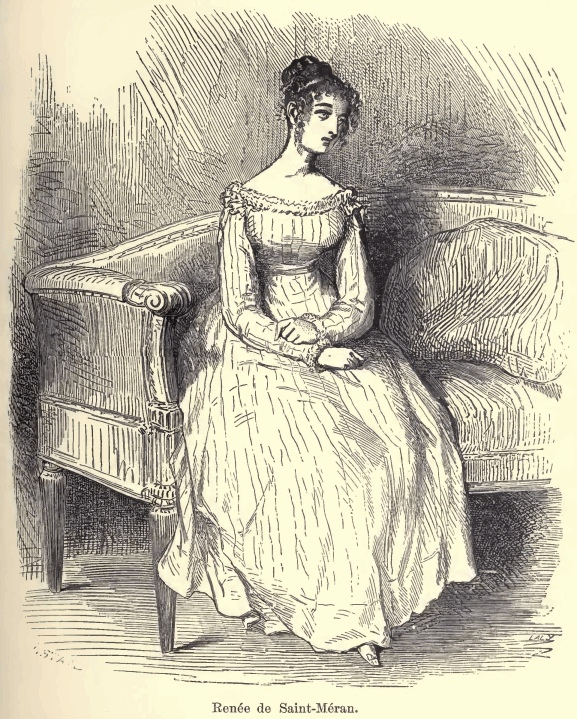
\includegraphics[width=\textwidth]{0091m.jpg}
\end{figure}

“That is true,” answered the marquis.

“How much do I owe this gracious prince! What is there I would not do
to evince my earnest gratitude!”

“That is right,” cried the marquise. “I love to see you thus. Now,
then, were a conspirator to fall into your hands, he would be most
welcome.”

“For my part, dear mother,” interposed Renée, “I trust your wishes will
not prosper, and that Providence will only permit petty offenders, poor
debtors, and miserable cheats to fall into M. de Villefort’s
hands,—then I shall be contented.”

“Just the same as though you prayed that a physician might only be
called upon to prescribe for headaches, measles, and the stings of
wasps, or any other slight affection of the epidermis. If you wish to
see me the king’s attorney, you must desire for me some of those
violent and dangerous diseases from the cure of which so much honor
redounds to the physician.”

At this moment, and as though the utterance of Villefort’s wish had
sufficed to effect its accomplishment, a servant entered the room, and
whispered a few words in his ear. Villefort immediately rose from table
and quitted the room upon the plea of urgent business; he soon,
however, returned, his whole face beaming with delight. Renée regarded
him with fond affection; and certainly his handsome features, lit up as
they then were with more than usual fire and animation, seemed formed
to excite the innocent admiration with which she gazed on her graceful
and intelligent lover.

“You were wishing just now,” said Villefort, addressing her, “that I
were a doctor instead of a lawyer. Well, I at least resemble the
disciples of Esculapius in one thing [people spoke in this style in
1815], that of not being able to call a day my own, not even that of my
betrothal.”

“And wherefore were you called away just now?” asked Mademoiselle de
Saint-Méran, with an air of deep interest.

“For a very serious matter, which bids fair to make work for the
executioner.”

“How dreadful!” exclaimed Renée, turning pale.

“Is it possible?” burst simultaneously from all who were near enough to
the magistrate to hear his words.

“Why, if my information prove correct, a sort of Bonapartist conspiracy
has just been discovered.”

“Can I believe my ears?” cried the marquise.

“I will read you the letter containing the accusation, at least,” said
Villefort:

“‘The king’s attorney is informed by a friend to the throne and the
religious institutions of his country, that one named Edmond Dantès,
mate of the ship \textit{Pharaon}, this day arrived from Smyrna, after having
touched at Naples and Porto-Ferrajo, has been the bearer of a letter
from Murat to the usurper, and again taken charge of another letter
from the usurper to the Bonapartist club in Paris. Ample corroboration
of this statement may be obtained by arresting the above-mentioned
Edmond Dantès, who either carries the letter for Paris about with him,
or has it at his father’s abode. Should it not be found in the
possession of father or son, then it will assuredly be discovered in
the cabin belonging to the said Dantès on board the \textit{Pharaon}.’”

“But,” said Renée, “this letter, which, after all, is but an anonymous
scrawl, is not even addressed to you, but to the king’s attorney.”

\begin{figure}[h]
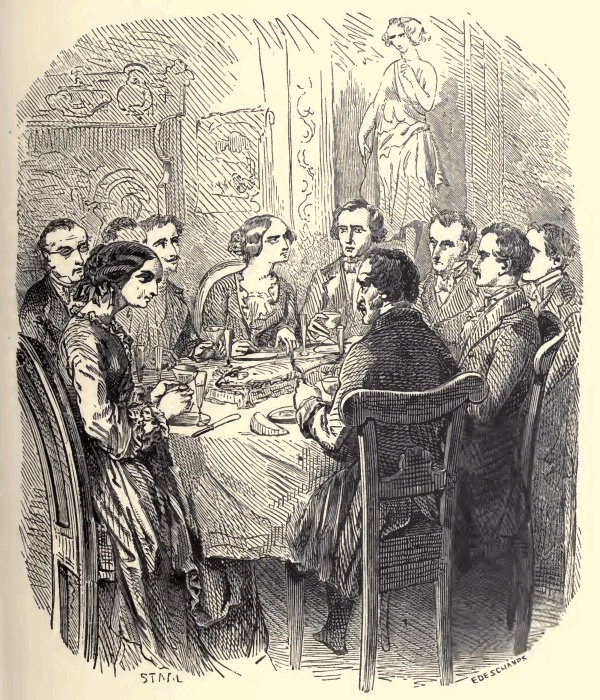
\includegraphics[width=\textwidth]{0093m.jpg}
\end{figure}

“True; but that gentleman being absent, his secretary, by his orders,
opened his letters; thinking this one of importance, he sent for me,
but not finding me, took upon himself to give the necessary orders for
arresting the accused party.”

“Then the guilty person is absolutely in custody?” said the marquise.

“Nay, dear mother, say the accused person. You know we cannot yet
pronounce him guilty.”

“He is in safe custody,” answered Villefort; “and rely upon it, if the
letter is found, he will not be likely to be trusted abroad again,
unless he goes forth under the especial protection of the headsman.”

“And where is the unfortunate being?” asked Renée.

“He is at my house.”

“Come, come, my friend,” interrupted the marquise, “do not neglect your
duty to linger with us. You are the king’s servant, and must go
wherever that service calls you.”

“Oh, Villefort!” cried Renée, clasping her hands, and looking towards
her lover with piteous earnestness, “be merciful on this the day of our
betrothal.”

The young man passed round to the side of the table where the fair
pleader sat, and leaning over her chair said tenderly:

“To give you pleasure, my sweet Renée, I promise to show all the lenity
in my power; but if the charges brought against this Bonapartist hero
prove correct, why, then, you really must give me leave to order his
head to be cut off.”

Renée shuddered at the word \textit{cut}, for the growth in question had a
head.

“Never mind that foolish girl, Villefort,” said the marquise. “She will
soon get over these things.” So saying, Madame de Saint-Méran extended
her dry bony hand to Villefort, who, while imprinting a son-in-law’s
respectful salute on it, looked at Renée, as much as to say, “I must
try and fancy ’tis your dear hand I kiss, as it should have been.”

“These are mournful auspices to accompany a betrothal,” sighed poor
Renée.

“Upon my word, child!” exclaimed the angry marquise, “your folly
exceeds all bounds. I should be glad to know what connection there can
possibly be between your sickly sentimentality and the affairs of the
state!”

“Oh, mother!” murmured Renée.

“Nay, madame, I pray you pardon this little traitor. I promise you that
to make up for her want of loyalty, I will be most inflexibly severe;”
then casting an expressive glance at his betrothed, which seemed to
say, “Fear not, for your dear sake my justice shall be tempered with
mercy,” and receiving a sweet and approving smile in return, Villefort
departed with paradise in his heart.

\printpagenotes*

\end{document}
